%        File: covo.tex
%     Created: Di Okt 16 10:00  2018 C
% Last Change: Di Okt 16 10:00  2018 C
%

\documentclass[a4paper]{report}
% ***************************PACKAGES***************************
\usepackage[Bjornstrup]{fncychap}
\usepackage{graphicx}
\usepackage{graphbox}
\usepackage{caption,setspace}
\usepackage{subcaption}
\captionsetup[figure]{width=0.7\textwidth,font={small}}
\usepackage{float}
\usepackage{amsmath}
\usepackage{amssymb}
\usepackage{hyperref}
\usepackage{siunitx}
\usepackage{graphicx}
\usepackage{mwe}
\usepackage{tabularx}
%\usepackage{cite}
\usepackage[
    backend=biber,
    parentracker=true,
    style=authoryear
  ]{biblatex}
  \addbibresource{../covo.bib}
\usepackage{hyperref}
\usepackage{bookmark}
\usepackage{algorithm}
\usepackage[noend]{algpseudocode}
\usepackage{array}
\usepackage{mathtools}
%\usepackage[titletoc]{appendix}
\usepackage{appendix}
\usepackage{multirow}

% ***************************NEW COMMANDS***************************
% for numbering per section
\numberwithin{figure}{section}
% removing ugly colored rectangles from references
\usepackage{xcolor}
\hypersetup{
    hidelinks,
    colorlinks = false,
    %linkcolor={black},
    %citecolor={black},
    %urlcolor={black}
  }
% command for table tabular alignment
\newcolumntype{L}{>{\raggedright\arraybackslash}X}
% command for argmin and argmax
%\DeclareMathOperator*{\argmax}{arg\,max}
%\DeclareMathOperator*{\argmin}{arg\,min}
\newcommand{\argmin}{\mathop{\mathrm{argmin}}}
\newcommand{\argmax}{\mathop{\mathrm{argmax}}}
\newcommand{\R}{\mathbb{R}}
% commands for cascading subfigures
\newsavebox{\subfloatbox}
\newcommand{\topfloat}[2][\empty]% #1 = caption, #2=image
 {\savebox\subfloatbox{#2}%
  \begin{minipage}[t]{\wd\subfloatbox}
    \usebox\subfloatbox
    \subcaption{#1}
  \end{minipage}}
\newcommand{\bottomfloat}[2][\empty]% #1 = caption, #2=image
 {\savebox\subfloatbox{#2}%
  \begin{minipage}[b]{\wd\subfloatbox}
    \captionsetup{position=top}%
    \subcaption{#1}
    \usebox\subfloatbox
  \end{minipage}}

\algnewcommand\algorithmicforeach{\textbf{for each}}
\algdef{S}[FOR]{ForEach}[1]{\algorithmicforeach\ #1\ \algorithmicdo}

\newcommand*{\vertbar}{\rule[-1ex]{0.5pt}{2.5ex}}
\newcommand*{\horzbar}{\rule[.5ex]{2.5ex}{0.5pt}}

% config for turning () to [] in citation
\newrobustcmd*{\parentexttrack}[1]{%
	\begingroup
	\blx@blxinit
	\blx@setsfcodes
	\blx@bibopenparen#1\blx@bibcloseparen
	\endgroup}

\AtEveryCite{%
	\let\parentext=\parentexttrack%
	\let\bibopenparen=\bibopenbracket%
	\let\bibcloseparen=\bibclosebracket}

%% config for appendix spacing in toc
%\setlength{\cftchapnumwidth}{2em}
%\cftsetindents{section}{2em}{2.4em}
%\cftsetindents{subsection}{4.4em}{3.2em}
%\DeclareTOCStyleEntry[indent=0pt]{tocline}{figure}
%\DeclareTOCStyleEntry[indent=0pt]{tocline}{table}

% ***************************ACRONYM AND SYMBOL DEFINITIONS*******************

\usepackage[acronym,nonumberlist,toc]{glossaries}
\makenoidxglossaries
% Acronyms
\newacronym{vo}{VO}{Visual Odometry}
\newacronym{slam}{SLAM}{Simultenous Localization and Mapping}
\newacronym{rgbd}{RGB-D}{RGB Color Camera with Depth Sensor}
\newacronym{imu}{IMU}{Inertial Measurement Unit}
\newacronym{ir}{IR}{Infrared}
\newacronym{dlt}{DLT}{Direct Linear Transformation}
\newacronym{sift}{SIFT}{Scale-Invarient Feature Transform}
\newacronym{surf}{SURF}{Speed-up Robust Features}
\newacronym{fast}{FAST}{Feature From Accelerated Segment Test}
\newacronym{brief}{BRIEF}{Binary Robust Independent Elementary Features}
\newacronym{orb}{ORB}{Oriented FAST and Rotated BRIEF}
\newacronym{ransac}{RANSAC}{Random Sample Consensus}
\newacronym{sfm}{SFM}{Structure from Motion}
\newacronym{icp}{ICP}{Iterative Closest Point}
\newacronym{dvo}{DVO}{Dense Visual Odometry}
\newacronym{covo}{CoVO}{Covariance-enabled Visual Odometry}
\newacronym{rmse}{RMSE}{Root Mean Squared Error}
\newacronym{rpe}{RPE}{Relative Pose Error}
\newacronym{nees}{NEES}{Normalized Estimation Error Squared}
\newacronym{anees}{ANEES}{Average Normalized Estimation Error Squared}

% Symbols
\newglossaryentry{world_coord}{
  name = \ensuremath{\mathcal{W}},
  description = index for the world coordinate system
}
\newglossaryentry{cam_coord}{
  name = \ensuremath{\mathcal{C}},
  description = index for the camera coordinate system
}
\newglossaryentry{disparity_space}{
  name = \ensuremath{\mathcal{D}},
  description = index for the disparity image space
}
\newglossaryentry{state_vector}{
  name = \ensuremath{\mathbf{x}},
  description = unknown state vector 
}
\newglossaryentry{desired_state_vector}{
  name = \ensuremath{\mathbf{x^*}},
  description = desired state vector 
}
\newglossaryentry{cam_position}{
  name = \ensuremath{\mathbf{p}},
  description = position vector in $\R^3$
}
\newglossaryentry{cam_orientation}{
  name = \ensuremath{\mathbf{q}},
  description = quaternion vector in $SO(3)$
}
%\newglossaryentry{transformation}{
%  name = \ensuremath{\mathbf{T}_{k,k+1}},
%  description = camera transformation from $k^{th}$ to $k+1^{th}$ frame
%}
\newglossaryentry{translation}{
  name = \ensuremath{\mathbf{t}},
  description = translation vector in $\R^3$
}
%\newglossaryentry{rotation}{
%  name = \ensuremath{\mathbf{q}_{k,k+1}},
%  description = camera rotation from $k^{th}$ to $k+1^{th}$ frame
%}
\newglossaryentry{2d_feature_pix_coord}{
  name = \ensuremath{\mathbf{u}},
  description = pixels coordinates of 2D image feature
}
\newglossaryentry{3d_point_cam_coords}{
  name = {\ensuremath{\mathbf{X}}} ,
  description = position of 3D point feature 
}
%\newglossaryentry{3d_point_world_coords}{
%  name = $\mathbf{X^{\mathcal{W}}}^{(i)}$ ,
%  description = $i^{th}$ 3D feature point's position coordinates
%  in world coordinate system
%}
\newglossaryentry{instrinsic}{
  name = {\ensuremath{\mathbf{K}}} ,
  description = instrinsic matrix
}
%\newglossaryentry{transformation}{
%  name = $\mathbf{T}$,
%  description = homogeneous transformation
%}
\newglossaryentry{transformation_ab}{
  name = $\mathbf{T}_{A,B}$,
  description = homogeneous transformation representing frame $A$ with respect 
  to frame $B$ in $SE(3)$
}
\newglossaryentry{projection}{
  name = {\ensuremath{\mathbf{P}}} ,
  description = projection matrix
}
\newglossaryentry{projection_func}{
  name = {\ensuremath{\mathbf{F_{p}}}} ,
  description = projection function
}
\newglossaryentry{back_proj}{
	name = {\ensuremath{\mathbf{F_{bp}}}} ,
	description = back-projection function
}
\newglossaryentry{distortion_func}{
  name = {\ensuremath{\mathbf{F_{d}}}} ,
  description = distortion function
}
\newglossaryentry{distort_projection_func}{
  name = {\ensuremath{\mathbf{F_{dp}}}} ,
  description = projection function combined with distortion effect
}
\newglossaryentry{depth_func}{
  name = {\ensuremath{F_d}} ,
  description = function that converts diparity value to metric depth
}
\newglossaryentry{homography}{
  name = {\ensuremath{\mathbf{H}}} ,
  description = homography matrix
}
\newglossaryentry{residuals_forward}{
	name = {\ensuremath{\mathbf{r_f}}} ,
	description = residuals function of forward-transformation
}
\newglossaryentry{residuals_backward}{
	name = {\ensuremath{\mathbf{r_b}}} ,
	description = residuals function of backward-transformation
}
\newglossaryentry{cov_uvz}{
	name = {\ensuremath{\mathbf{Q_{uvz}}}} ,
	description = 3D point feature covariance in $\mathcal{D}$
}
\newglossaryentry{cov_xyz}{
	name = {\ensuremath{\mathbf{Q_{xyz}}}} ,
	description = 3D point feature covariance in $\mathcal{C}$
}
\newglossaryentry{cov_tq}{
	name = {\ensuremath{\mathbf{Q_{tq}}}} ,
	description = 3D pose covariance in $\mathcal{C}$
}
\newglossaryentry{pixel_uncertainty}{
name = {\ensuremath{\sigma_u, \sigma_v}} ,
description = pixels noise variance
}
\newglossaryentry{depth_axial_uncertainty}{
	name = {\ensuremath{\sigma_Z}} ,
	description = axial depth noise variance
}
\newglossaryentry{lateral_axial_uncertainty}{
	name = {\ensuremath{\sigma_L}} ,
	description = lateral depth noise variance
}
\newglossaryentry{back_proj_jacob}{
	name = {\ensuremath{\mathbf{J_{bp}}}} ,
	description = Jacobian matrix of back-projection function
}
\newglossaryentry{back_trans_jacob}{
	name = {\ensuremath{\mathbf{J_{b}}}} ,
	description = Jacobian matrix of back-transformation function
}
\newglossaryentry{for_trans_jacob}{
	name = {\ensuremath{\mathbf{J_{f}}}} ,
	description = Jacobian matrix of forward-transformation function
}
\newglossaryentry{residuals_jacob}{
	name = {\ensuremath{\mathbf{J_{tq}}}} ,
	description = Jacobian matrix of residuals function of both 
	backward-transformation and forward-transformation
}
\newglossaryentry{residuals_scaled_info_jacob}{
	name = {\ensuremath{\mathbf{J_{tqs}}}} ,
	description = Jacobian matrix of residuals function of both 
	backward-transformation and forward-transformation scaled by information 
	matrix
}
\newglossaryentry{residuals_scaled_manifold_jacob}{
	name = {\ensuremath{\mathbf{J_{tqm}}}} ,
	description = Jacobian matrix of residuals function of both 
	backward-transformation and forward-transformation scaled by manifold
}
\newglossaryentry{residuals_scaled_info_manifold_jacob}{
	name = {\ensuremath{\mathbf{J_{tqsm}}}} ,
	description = Jacobian matrix of residuals function of both 
	backward-transformation and forward-transformation scaled by both 
	information matrix and manifold
}


\renewcommand{\contentsname}{Table of Contents}

% ***************************DOC***************************
\begin{document}

% ***************************TITLE***************************
\begin{titlepage}
\begin{center}

%  
\includegraphics[width=\textwidth]{../fig/tuc_logo.jpg}

\vspace{1.5cm}


{\Huge \textbf{Master Thesis}}\\
\vspace{0.5cm}
{\huge \textbf{An Error-Aware RGB-D \\Visual Odometry}}


\vspace{2.5cm}

{\huge \textbf{U\u{g}ur Bolat}}

\vfill

Date:

\vspace{1.2cm}

Supervisors: \\
Dr.-Ing. Sven Lange \\
M.Sc. Tim Pfeifer

\vspace{0.8cm}

Faculty of Electrical Engineering and Information Technology\\
Professorship of Process Automation

\end{center}
\end{titlepage}

\begin{abstract}

% ***************************ABSTRACT***************************
% Soft intro to the problem
% talk about robustness
\textit{Robustness} of a robot can be defined as an ability to operate under
\textit{uncertainty} without the occurrence of a downtime. There are
well-designed robots whose task is to solve a defined problem without moving
from its assembled position.  They can operate safely because the uncertainty 
of
operational components and its controlled environment are modeled with
substantial accuracy and precision. However, once we build robots that move
around and interact with the real world, the number of unforeseen events increase
drastically. In such scenarios, robustness is crucial.  The way we increase
robustness is to have intelligent agents and accurate uncertainty models of
their sensors and estimations. That being said, this work focuses on the latter
and aims to investigate the uncertainty of RGB-D camera sensor in the context
of Visual Odometry (VO).

So far, researchers and engineers have developed many RGB-D camera based VO
applications.  In filter-based or graph-based SLAM applications, they are
usually combined with other dead-reckoning and landmark measurements because of
the drift occurring in relative pose estimations over time. In this respect, one
should have a reliable uncertainty model of the sensors being measured so that
the uncertainty of pose estimations can be estimated in the form of a covariance
matrix.  To my knowledge, there is no open source VO software that provides
such covariance matrices for its pose estimations. Thus, the covariance matrix
for VO is taken as an identity matrix. Nevertheless, this does not offer any metric 
uncertainty information as to whether the estimation should have specific importance
comparing to other sensor measurements during filtering or optimization
process.  On the other hand, researchers model the uncertainty of RGB-D cameras
such as Kinect, but they applied their models on applications that are outside
of VO.  The primary goal of this work is to build such a VO system that it
provides not only relative pose estimations but also a covariance matrix of its
estimated poses.  To achieve this goal, we estimate the covariance matrix of
the predicted pose by propagating metric uncertainty of 3D point features that
are modeled with the sensor characteristics of an RGB-D camera.


\end{abstract}

\newpage


% ***************************FRONTEND STUFF***************************

% Table of Contents
\pagenumbering{roman}
\tableofcontents
\cleardoublepage
\setcounter{page}{1}
\listoffigures
\addcontentsline{toc}{chapter}{\listfigurename}
\listoftables
\addcontentsline{toc}{chapter}{\listtablename}
\newpage
\printnoidxglossary[type=acronym,title={List of Abbreviations}]
\printnoidxglossary[title=List of Notations,sort=def]
\glsaddallunused
\printacronyms
\chapter*{Acknowledgement}
\addcontentsline{toc}{chapter}{Acknowledgments}
\newpage

% ***************************DOCUMENT***************************
\pagenumbering{arabic}

% ***************************CP1-INTRO***************************
\chapter{Introduction} \label{cp_intro}

The essence of a mobile robot is autonomy. 
A fully autonomous robot first \textit{senses} its environment, then 
\textit{interprets} the collected data and finally \textit{acts} based on the insights 
that it gathered over time.
If we look at nature, throughout evolution, 
certain animals gained certain abilities regarding 
spatial awareness in all sorts of ways. For instance, 
homing pigeons navigate by a magnetic field. Bats use sound to map their 
surroundings. Bees smell with their special chemoreception to find their way 
back home. 
Even though each sense helps us with particular importance,
we humans are good at navigating ourselves by relying on our vision. 
While the incredible capability of human vision and perception 
mostly stay a mystery, 
robotics researchers have naturally been drawn to studying 
the computer vision field for navigation purposes.


% General intro to the problem
For a mobile robot to act autonomously in the real world, the state of the
robot must be known accurately. We define this physical state by its
\textit{pose}, meaning its position and orientation. The current pose of the
robot can be measured by two ways; i.e., \textit{dead-reckoning} that measures
\textit{relative} motion and \textit{landmarks} that measures \textit{absolute}
position which is known a priori.  Without priori-known landmark measurements,
dead-reckoning systems are destined to drift from its real position. Thus, the
robot must build a map of its environment along with the previously seen
landmarks. Then, it will have a chance to recover from drifts by recognizing
the same landmarks in the same area at different time. In fact, this problem in
robotics is named as \acrfull{slam}. SLAM problem has almost 30 years history
\parencite{Moravec1980} and vision systems always had great importance. Even 
though
some researchers \parencite{Frese2010} consider SLAM to be solved, there are 
still
open research questions regarding robustness, accuracy and real-time operation.

% Sensor fusion importance
To solve SLAM problems, robots are equipped with various kind of sensors 
such as 
dead-reckoning sensors; e.g., IMU, wheel odometry and visual odometry. 
Each sensor comes with its own benefits and limitations. For example, 
wheel odometry offers a cheap and simple solution, but 
it is hard to model non-deterministic slippery motions. 
On the other hand, visual odometry (VO) is more agile and accurate compared to 
wheel odometry. However, 
for the VO system to work
accurately with the current algorithms, the environment should be adequately 
illuminated, static and
texture-rich.  However, we deal with shadowed, dynamic and
texture-poor environments in the real world. Eventually, drifts will occur in 
VO. 
Hence, the good
design of a mobile robot should combine many sensors.
In fact, combining a variety of sensors 
along with their known biases and calibration parameters is called 
\textit{sensor fusion}.

Nowadays, sensor fusion applications for SLAM and 3D reconstruction are designed 
accordingly to compensate each other's biases in order to obtain the best 
possible result. In the case of an accurate and robust sensor fusion framework, 
one selects a sufficient amount absolute and relative positioning sensors. 
The main goal is to fuse both relative and absolute sensor types 
along with their noise characteristics in a way that the error is minimized. 
Hence, it is critical to model each sensor's uncertainties. 
IMU and wheel odometry sensors' uncertainty is modeled by their vendors 
based on the working principles and worst-case scenario tests beforehand.
Whereas, widely used open source VO tools do not provide any uncertainty information 
about their pose estimations. Even though there are several VO papers 
\parencite{Endres2014}, \parencite{Konolige08}, \parencite{Di2016a}, 
\parencite{Belter2018a}
that deals with the uncertainty of RGB-D sensors, they only intend to 
improve the accuracy of the pose estimation, but not to provide any 
uncertainty 
information about their estimation. Therefore, the ultimate motivation, in 
this thesis, is to build 
a feature-based RGB-D Visual Odometry system that outputs pose estimations 
along with their metric uncertainties.
As a result, the VO system can be treated as a stand-alone 
odometry system that is ready to fuse with other sensors.


% Outline the thesis?
The overall structure of the thesis takes the form of six chapters, including
this introductory chapter. In Chapter 2, we study the essential geometrical
models and calibration techniques for an RGB-D camera. Then, Chapter 3 outlines
the standard feature-based VO pipeline and explains the necessary image
processing methods for building such a pipeline. In Chapter 4, we discuss how
to model the uncertainty of an RGB-D camera and integrate this model into the
VO pipeline so that the uncertainty of a pose estimation can be calculated.
Afterward, we evaluate the accuracy and consistency of the proposed VO system
with both simulated data and TUM RGB-D dataset in Chapter 5. Finally, the
conclusion gives a summary and critique of the findings.


% ***************************CP2-VO***************************


\chapter{Camera Models} \label{cp_cam_models}

% RGB-D Camera in VO?
The camera offers rich data by mapping 3D
space onto a 2D plane and the output data are quantized pixels according to the
intensity of the illumination.  This type of data makes a camera a
multi-purpose device so one can build various kinds of computer vision
applications.  Considering the potential, computer vision researchers proposed
VO methods that are tailored to different type of environments.  When
designing a VO pipeline, one should select a suitable algorithm and camera type
based on the operating environment.

% Why used? Advantages?
As to camera types, RGB-D cameras based on structured light (e.g., PrimeSense
Carmine, Microsoft Kinect (see Figure \ref{fig:kinect_pic}), and Asus Xtion) 
that are categorized as active
stereo cameras are especially intriguing.  These cameras gave rise to many 3D
vision applications including VO. Even though it has certain limitations; i.e.,
the depth accuracy being grown with distance to the object, it offers cheap 3D 
data, especially for
indoor applications. 


In this chapter, we will discuss two geometrical model and calibration methods
for an RGB-D camera.  In principle, a camera maps from a 3D world scene to a 2D
image plane. We call this process \textit{projection} operation. Since the VO
systems process projected image sequences, one has to model this projection
operation accurately. One of the basic camera modeling technique is the
\textit{pinhole model} where the projection of the 3D points is mapped on a 2D
image plane.  

\begin{figure}[H]
	\centering
	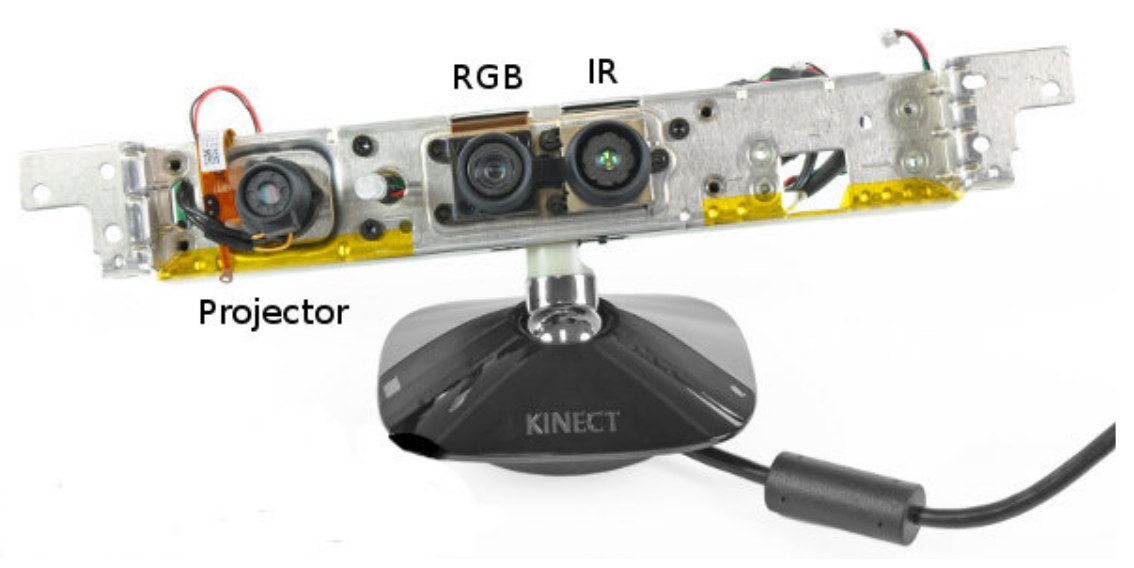
\includegraphics[width=0.65\linewidth,natwidth=640,natheight=640]
	{fig/ref_imgs/kinect_pic.png}
  \caption[Microsoft Kinect V1]{Microsoft Kinect V1 is an RGB-D camera that 
  has 
  640 $\times$ 480 pixels spatial resolution, 0.8-4.0 $m$ depth range, 2-40 
  $mm$ depth resolution, and 30 fps \parencite{Smisek2011}.}
	\label{fig:kinect_pic}
\end{figure}

While mapping a point from 3D space to 2D space, we lose the 
depth information.  Although there are ways to recover the relative depth 
scale by 
taking images from different poses with a monocular camera, they can't provide 
metric depth.  In this thesis, we are interested in cameras that offer metric 
depth using stereo camera principle, more specifically active stereo camera. 
Thus, one 
can 
model these active stereo cameras with the \textit{triangulation model}. That 
being said, these two models cannot be used without having the camera to be 
\textit{calibrated} since many anomalies occur in manufacturing. In this 
chapter, we will discuss the geometric models of an RGB-D camera and how 
to calibrate it.


\section{The Pinhole Model} \label{sc_pinhole}

The light rays are captured through the camera's lens onto an electronic plate 
(called \textit{image plane} in computer vision) that converts light intensity 
to electrical signals.  The pinhole model is, on the other hand, an 
approximation to this operation.  In this model, the camera 
center sits behind the image plane.  The z-axis, so-called \textit{principal 
axis}, of this coordinate system points out through the origin of the image 
plane. Also, the point where pierce through image plane is called the 
\textit{principal point} $\mathbf{p}$. In Figure \ref{fig:pinhole}, we can see 
how other two axes; 
i.e., X and Y, are located and the depicted coordinate system is known as 
the \textit{camera coordinate system}. Note that the formulation of the 
pinhole model was mostly taken from \parencite{RichardHartley2003}.


\begin{figure}[H]
	\centering
	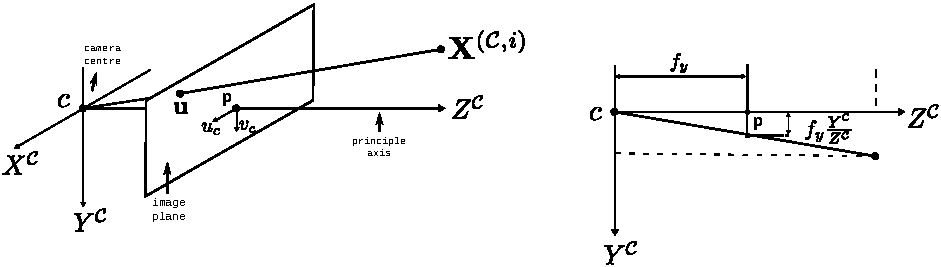
\includegraphics[width=\linewidth,natwidth=640,natheight=640]
  {fig/drawings/pinhole_3d2d.pdf}
  \caption[The Pinhole Model]{In the pinhole model, $C$ is the camera center 
  and $\mathbf{p}$ is the principle point. A 3D point 
  $\mathbf{X^{\mathcal{C}}}$ in the 
  camera coordinate system is projected as a 2D point $\mathbf{u}$ onto the 
  image plane. Note that the camera coordinate system is drawn according to 
  right-hand rule. The illustration is redrawn from 
  \parencite{RichardHartley2003} 
  accordingly.}
	\label{fig:pinhole}
\end{figure}

Thanks to geometrical proportion property, we can project the 3D point 
$\mathbf{X^{\mathcal{C}}}=(X^{\mathcal{C}}, Y^{\mathcal{C}}, 
Z^{\mathcal{C}})^\top$ in the 
camera 
coordinate system 
to 
the 2D 
point $\mathbf{u} = (f_xX^{\mathcal{C}}/Z^{\mathcal{C}}, 
f_yY^{\mathcal{C}}/Z^{\mathcal{C}})^\top$ on the 
image 
plane, where 
$f_x$ and $f_y$ are the \textit{focal lengths} between the camera center and 
the principal point with respect to horizontal and vertical axis of the camera 
coordinate system respectively.  After projection, we obtain a 2D point  
as \textit{pixel coordinates} $\mathbf{u}=(u,v)^\top$ on the image 
plane.  To 
be more specific, we can write the projection operation as a linear mapping 
function in the following way if we utilize the homogeneous coordinates:

\begin{equation}
  \begin{pmatrix}
    u\\
    v\\
    1
  \end{pmatrix}
  \sim
  Z^{\mathcal{C}}
  \begin{pmatrix}
    f_x\frac{X^{\mathcal{C}}}{Z^{\mathcal{C}}}\\
    f_y\frac{Y^{\mathcal{C}}}{Z^{\mathcal{C}}}\\
    1
  \end{pmatrix}
  =
  \begin{pmatrix}
    f_xX^{\mathcal{C}}\\
    f_yY^{\mathcal{C}}\\
    Z^{\mathcal{C}}
  \end{pmatrix}
  =
  \begin{bmatrix}
    f_x & 0 & 0 & 0\\
    0 & f_y & 0 & 0\\
    0 & 0 & 1 & 0\\
  \end{bmatrix}
  \begin{pmatrix}
    X^{\mathcal{C}}\\
    Y^{\mathcal{C}}\\
    Z^{\mathcal{C}}\\
    1
  \end{pmatrix}
\end{equation} \label{eq:proj_func_w_f}

This equation applies for the case when 3D points are projected onto a plane 
where the principal point is the origin.  However, the common convention in 
practice is to have the origin at the corner \parencite{RichardHartley2003}, 
instead of the center (see Figure \ref{fig:pinhole_offset}).

\begin{figure}[H]
	\centering
  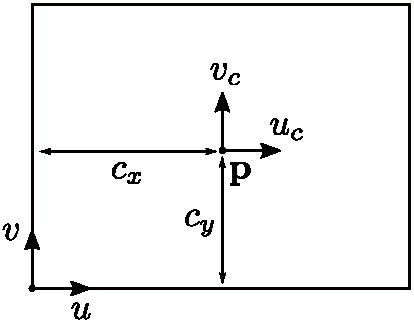
\includegraphics[width=0.4\linewidth,natwidth=640,natheight=640]
  {fig/drawings/pinhole_cam_offset.pdf}
	\caption[Principle Point Offset]{We take OpenCV's pixel coordinate 
	convention where the origin is located at the upper left corner. In order 
	to shift the origin from the camera center to the corner, $c_x, c_y$ 
	principle 
	point offsets are added.}
	\label{fig:pinhole_offset}
\end{figure}

Thus, we get offsets, which can further be added as:

\begin{equation}
  \begin{pmatrix}
    u\\
    v\\
    1
  \end{pmatrix}
  \sim
  Z^{\mathcal{C}}
  \begin{pmatrix}
    \frac{f_x X^{\mathcal{C}} + Z^{\mathcal{C}} c_x}{Z^{\mathcal{C}}}\\
    \frac{f_y Y^{\mathcal{C}} + Z^{\mathcal{C}} c_y}{Z^{\mathcal{C}}}\\
    1
  \end{pmatrix}
  =
  \begin{pmatrix}
    f_xX^{\mathcal{C}} + Z^{\mathcal{C}} c_x\\
    f_yY^{\mathcal{C}} + Z^{\mathcal{C}} c_y\\
    Z^{\mathcal{C}}
  \end{pmatrix}
  =
  \begin{bmatrix}
    f_x & 0 & c_x & 0\\
    0 & f_y & c_y & 0\\
    0 & 0 & 1 & 0\\
  \end{bmatrix}
  \begin{pmatrix}
    X^{\mathcal{C}}\\
    Y^{\mathcal{C}}\\
    Z^{\mathcal{C}}\\
    1
  \end{pmatrix}\label{eq:proj_func_w_f_c}
\end{equation} 

where $c_x$ and $c_y$ are coordinates of the principal point \textbf{p}.
In addition to principal offsets, an inaccurately synchronized pixel-sampling 
process can result in \textit{skewed pixels}. This camera imperfection leads 
to non-square pixels as seen in Figure \ref{fig:skewed}.

\begin{figure}[H]
	\centering
  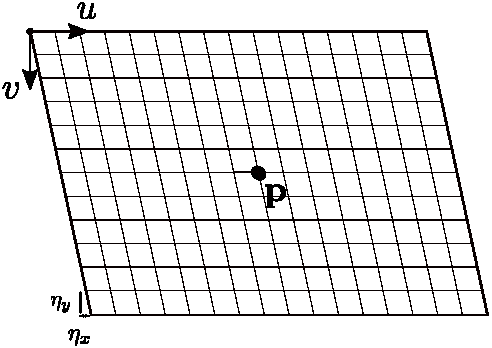
\includegraphics[width=0.4\linewidth,natwidth=640,natheight=640]
  {fig/drawings/pinhole_skew.pdf}
  \caption[Skewed Pixels]{Skewed pixels occur in earlier versions of CCD 
  cameras because the camera's detector array was not orthogonal to the 
  principle axis. This design issue is mostly fixed in modern camera and thus 
  it is usually neglected by taking $\eta_x=1$, $\eta_y=1$ and $s=0$.}
	\label{fig:skewed}
\end{figure}

We can scale the square pixels, having 1:1 pixel aspect ratio, with the 
corresponding skew parameters $\eta_x$, $\eta_y$ and $s$:

\begin{equation} \label{eq:proj_func_w_square_pix_skew}
  \begin{pmatrix}
    u\\
    v\\
    1
  \end{pmatrix}
  \sim
  \begin{bmatrix}
    f_x\eta_x & s & c_x & 0\\
    0 & f_y\eta_y & c_y & 0\\
    0 & 0 & 1 & 0\\
  \end{bmatrix}
  \begin{pmatrix}
    X^{\mathcal{C}}\\
    Y^{\mathcal{C}}\\
    Z^{\mathcal{C}}\\
    1
  \end{pmatrix}
  =
  \begin{bmatrix}
    \alpha_x & s & c_x & 0\\
    0 & \alpha_y & c_y & 0\\
    0 & 0 & 1 & 0\\
  \end{bmatrix}
  \begin{pmatrix}
    X^{\mathcal{C}}\\
    Y^{\mathcal{C}}\\
    Z^{\mathcal{C}}\\
    1
  \end{pmatrix}
\end{equation} 

At this point, we can extract the following matrix:

\begin{equation}
  \mathbf{K_{RGB}} = 
  \begin{bmatrix}
    \alpha_x & s & c_x\\
    0 & \alpha_y & c_y\\
    0 & 0 & 1\\
  \end{bmatrix}\label{eq:k_matrix}
\end{equation} 

where $\mathbf{K_{RGB}}$ is called \textit{intrinsic matrix}, which represents 
the characteristics of a camera sensor.  With this matrix, one can further 
reformulate the notation \eqref{eq:proj_func_w_square_pix_skew} in more 
compact 
form:

\begin{equation}\label{eq:simplyfied_proj_func}
  \mathbf{u} = \mathbf{K_{RGB}}[\mathbf{I}|\mathbf{0}]\mathbf{X^{\mathcal{C}}}
\end{equation} 

\begin{figure}[H]
	\centering
  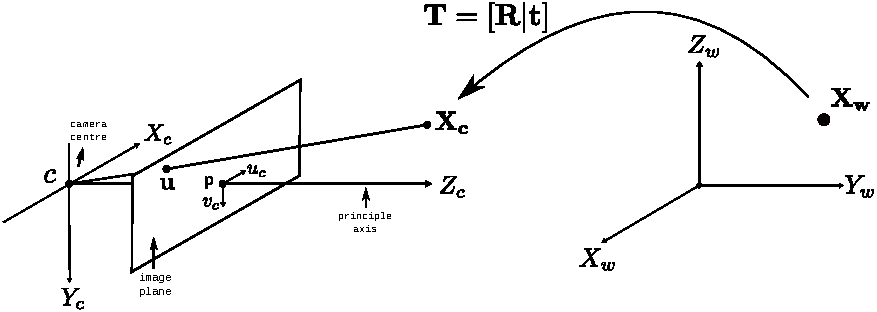
\includegraphics[width=\linewidth,natwidth=640,natheight=640]
  {fig/drawings/pinhole_world_to_cam.pdf}
  \caption[Extrinsic Matrix]{The z-axis of the camera coordinate system aligns 
  with the principal axis that is \textit{local} to the camera frame. In fact, 
  we 
  have measured 3D points that we know their position in the \textit{world 
  coordinate system} which is also referred to the \textit{global frame}, as 
  opposed to the camera coordinate system referring to the 
\textit{local frame}.}
  \label{fig:cam_model_rot_trans}
\end{figure}

Remember that we measure 3D points in the real world with respect to the 
camera center.  Thus, these two coordinates systems, i.e., the camera and 
world coordinate system, can be transformed one another by a rotation and a 
translation as it is depicted in Figure \ref{fig:cam_model_rot_trans} and we 
are interested in converting from the world coordinate system to the camera 
coordinate system in the context of projection operation.  In this regard, we 
perform series of rotations around each axis of the Cartesian coordinate 
system in $\R^3$ Euclidean space by using \textit{rotation matrices} where 
$R_x, R_y, R_z \in SO(3)$ is the rotation group:

\begin{equation}
  R_x(\alpha) = 
  \begin{bmatrix}
    1 & 0 & 0\\
    0 & cos\alpha & -sin\alpha\\
    0 & sin\alpha & cos\alpha
  \end{bmatrix}\label{eq:rot_matrx_x}
\end{equation} 

\begin{equation}
  R_y(\beta) = 
  \begin{bmatrix}
    cos\beta & 0 & -sin\beta\\
    0 & 1 & 0\\
    sin\beta & 0 & cos\beta
  \end{bmatrix}\label{eq:rot_matrx_y}
\end{equation} 

\begin{equation}
  R_z(\gamma) = 
  \begin{bmatrix}
    cos\gamma & -sin\gamma & 0\\
    sin\gamma & cos\gamma & 0\\
    0 & 0 & 1
  \end{bmatrix}\label{eq:rot_matrx_z}
\end{equation} 

Now, let's concatenate all three rotations about axes z, y, x respectively 
(also 
called \textit{yaw, pitch, yaw}) by the matrix multiplication:

\begin{equation}
  \mathbf{R}_{\mathcal{W}, \mathcal{C}} = 
  \mathbf{R_z(\gamma)}\mathbf{R_y(\beta)}\mathbf{R_x(\alpha)}
  =
  \begin{bmatrix}
    r_{11} & r_{12} & r_{13}\\
    r_{21} & r_{22} & r_{23}\\
    r_{31} & r_{32} & r_{33}\\
  \end{bmatrix}\label{eq:rot_matrix_derivation}
\end{equation} 

Then, we add a translation $\mathbf{t}_{\mathcal{W}, \mathcal{C}} \in 
\R^{3x1}$:

\begin{equation}
  \mathbf{t}_{\mathcal{W}, \mathcal{C}} = 
  \begin{bmatrix}
    t_x \\ t_y \\ t_z
  \end{bmatrix}\label{eq:translation}
\end{equation} 

For convenience, we stack the rotation matrix and the translation vector into 
one:

\begin{equation}
  {\mathbf{T_{RGB}}}_{\mathcal{W}, \mathcal{C}} =
  \begin{bmatrix}
    r_{11} & r_{12} & r_{13} & t_x\\
    r_{21} & r_{22} & r_{23} & t_y\\
    r_{31} & r_{32} & r_{33} & t_z\\
  \end{bmatrix}\label{eq:transformation_matrix}
\end{equation} 

where ${\mathbf{T_{RGB}}}_{\mathcal{W}, \mathcal{C}} \in \R^{4x3}$ matrix 
in $SE(3)$ represents a 
\textit{transformation} of a 3D position from the world coordinate system to 
the 
camera coordinate system, which we call \textit{extrinsic camera parameters}.  
Finally, we combine intrinsic $\mathbf{K_{RGB}}$ and extrinsic 
${\mathbf{T_{RGB}}}_{\mathcal{W}, \mathcal{C}}$ matrices in the following form:

\begin{equation}\label{eq:simplyfied_proj_func_1}
  \mathbf{u} = 
  \mathbf{P_{RGB}}\mathbf{X^{\mathcal{W}}} = 
  \mathbf{K_{RGB}}{\mathbf{T_{RGB}}}_{\mathcal{W}, 
  \mathcal{C}}\mathbf{X^{\mathcal{W}}} 
  = 
  \mathbf{K_{RGB}}[\mathbf{R}|\mathbf{t}]_{\mathcal{W}, 
  \mathcal{C}} \mathbf{X^{\mathcal{W}}} =
  \mathbf{K_{RGB}}\mathbf{X^{\mathcal{C}}}
\end{equation} 

where $\mathbf{P_{RGB}}$ is the \textit{projection matrix}. All of these 
series of linear operations can be written as a function too:

\begin{equation}\label{eq:simplyfied_proj_func_2}
  \mathbf{u} = \mathbf{F_{p}}(\mathbf{X^{\mathcal{W}}})
\end{equation} 

where $\mathbf{F_{p}}(\mathbf{X^{\mathcal{W}}})$ is the \textit{projection 
function}, 
which takes the 3D points in the world coordinate system, transforms to the 
camera coordinate systems and then maps them onto the image plane.

\begin{figure}[H]
\begin{tabular}{ccc}
\centering
\subcaptionbox{Undistorted Image}{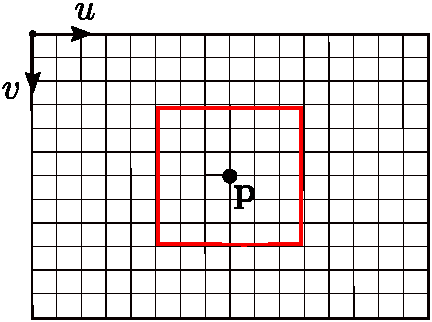
\includegraphics[width = 0.3\linewidth]{fig/drawings/pinhole_undistort.pdf}} &
\subcaptionbox{Barrel Distorted Image}{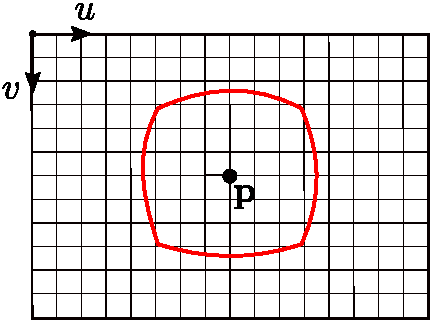
\includegraphics[width = 0.3\linewidth]{fig/drawings/pinhole_distort_1.pdf}}
\subcaptionbox{Pincushion Distorted Image}{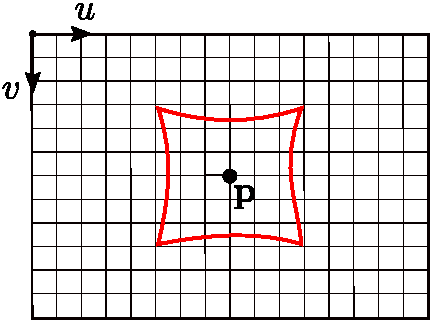
\includegraphics[width = 0.3\linewidth]{fig/drawings/pinhole_distort_2.pdf}}
\end{tabular}
\caption[Radial Distortion]{All emitted 
  lights through the camera lens is expected to intersect at the same 
  focus point and the radial distortion is caused by having a defected lens 
  that causes the emitted lights focusing different points.
  This makes the straight lines appear to be curved.}
\end{figure}\label{fig:}

One last issue with regards to imperfect pixels is the \textit{radial 
distortion}.  The distortion effect has non-linear characteristics. Thus, we 
introduce polynomial function whose coefficients $\kappa = (k_1, k_2, p_1, 
p_2, k_3)^\top$ can be fitted by optimization. The polynomial function is 
given 
as follows:

\begin{equation}
\begin{split}
  x'' = \mathbf{F_{d}}(x') = 
  x'(1+ k_1 r^2 + k_2 r^4 + k_3 r^6) + 2 p_1 x' y' + p_2 (r^2+2x'^2)\\
  y'' = \mathbf{F_{d}}(y') = 
  y'(1+ k_1 r^2 + k_2 r^4 + k_3 r^6) + p_1 (r^2+2y'^2) + 2p_2 x'y'\\
\end{split}
\end{equation}

where $x' = X^{\mathcal{C}}/Z^{\mathcal{C}}$ and $y' = 
Y^{\mathcal{C}}/Z^{\mathcal{C}}$. Now, we 
can update 
the 
projection function:

\begin{equation}
  \begin{pmatrix}
    u\\
    v\\
    1
  \end{pmatrix}
  =
  \begin{pmatrix}
    \alpha_x x'' + sy''+ c_x\\
    \alpha_y y'' + c_y\\
    1
  \end{pmatrix}
    =
    \mathbf{K_{RGB}}
    \mathbf{F_{d}}\begin{pmatrix}
       {\mathbf{T_{RGB}}}_{\mathcal{W}, \mathcal{C}}
      \begin{pmatrix}
        X^{\mathcal{W}}\\
        Y^{\mathcal{W}}\\
        Z^{\mathcal{W}}\\
        1
      \end{pmatrix}
    \end{pmatrix}\label{eq:proj_func_w_f_c}
\end{equation} 

Let's combine projection and distortion function into one:

\begin{equation}\label{eq:simplyfied_dist_proj_func}
  \mathbf{u} = \mathbf{F_{dp}}(\mathbf{X^{\mathcal{W}}})
\end{equation} 


To build any reliable computer vision application with digital cameras, it is 
essential to find the parameters of the projection matrix and the radial 
distortion.  Section \ref{sb_sc_rgb_calibration} describes one of many 
numerical methods for 
estimating them in literature.

\section{The Triangulation Model} \label{sc_depth_model}

Projected images captured by RGB cameras lack depth and angle information. To 
acquire this information, two main techniques are developed; e.g., passive 
stereo cameras and active stereo cameras. For passive stereo cameras, 
typically two synchronized cameras are placed horizontally with a known 
distance to each other. 
Whereas, for an active stereo camera, one typically has one light projector 
and one camera sensor. For example, in Kinect, an Infrared (IR) laser projects 
structured IR speckle light pattern on an object, and then the deformed light 
due to 3D geometry of the object is captured with a monochrome IR camera from 
a different position. Note that the formulation of the triangulation model is 
mostly constructed by using papers; i.e., \parencite{Park2012a} and 
\parencite{Khoshelham2012a}.

\begin{figure}[H]
	\centering
  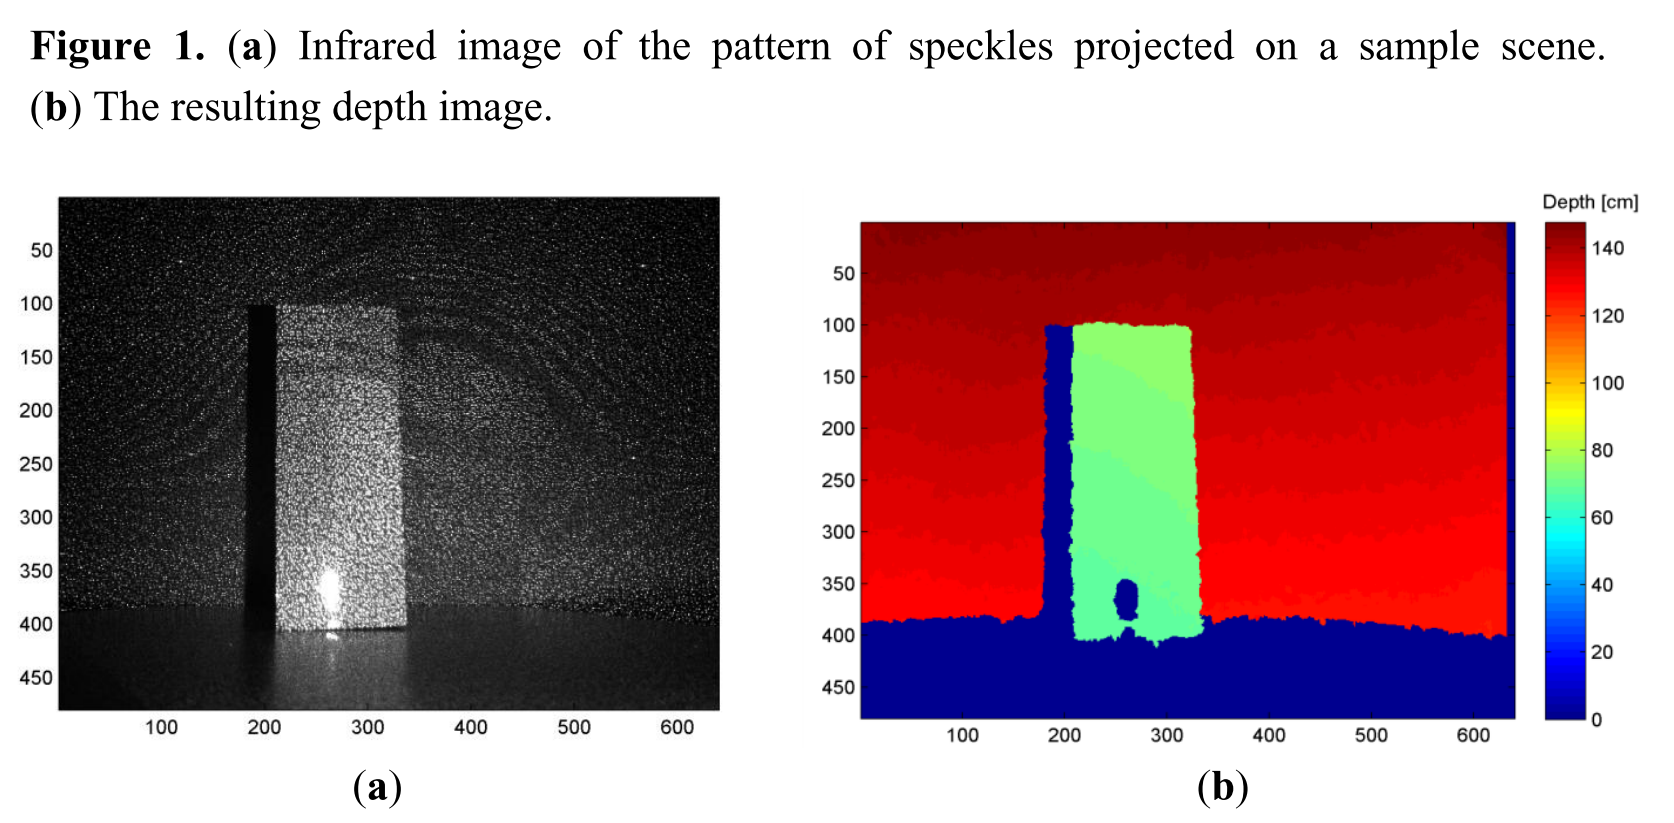
\includegraphics[width=0.7\linewidth,natwidth=640,natheight=640]
  {fig/ref_imgs/kinect_depth_img.png}
  \caption[Kinect's Depth Measurement]{On the left, the IR camera capture the 
  patterns of speckles projected on an object. On the right, we see the 
  resulting depth image if disparity data is converted accordingly 
  \parencite{Khoshelham2012a}.}
	\label{fig:kinect_depth_img}
\end{figure}

Since we use Kinect V1 to retrieve depth information for our experiments, we will 
be modeling active stereo vision principle even though the basic principle 
behind them is the same mathematical model, which is the \textit{triangulation 
model}. As shown in Figure \ref{fig:triangulation_model}, this model is a 
geometrical model that takes advantages of similarity triangles to calculate 
the depth.

\begin{figure}[H]
	\centering
  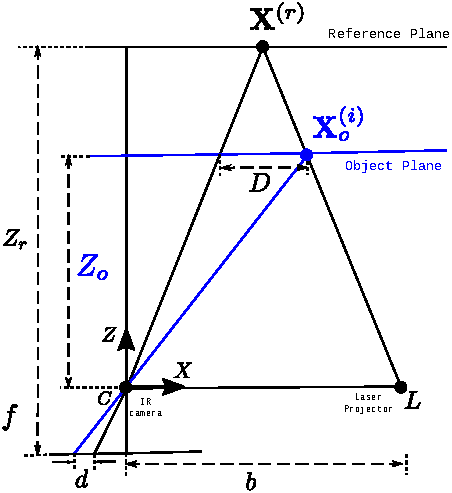
\includegraphics[width=0.65\linewidth,natwidth=640,natheight=640]
  {fig/drawings/triangulation.pdf}
  \caption[The Depth Measurement Model]{The Depth Measurement Model. The 
  illustration is redrawn from \parencite{Khoshelham2012a}.}
	\label{fig:triangulation_model}
\end{figure}

In this setup, we again utilize the camera coordinate system similar to RGB 
camera and IR camera with $f$ focal length is placed by facing perpendicular 
to the (principal axis) z-axis at the origin. Then, IR laser projector is also 
placed along the x-axis parallel to the IR camera with \textit{baseline} 
$b$ distance.  
Additionally, we measure $d$ as \textit{disparity} data and the maximum 
range that can be measured refers to $Z_r$. Ultimately, we are interested in 
finding $Z^{\mathcal{C}}$ distance if depth information of a point 
$\mathbf{X}^{\mathcal{C}}$ is 
desired. In this respect, we build two useful relationships using similarity 
of 
triangles:


\begin{equation}
  \frac{D}{b} = \frac{Z_r - Z^{\mathcal{C}}}{Z_r} \text{ and } \frac{d}{f} = 
  \frac{D}{Z^{\mathcal{C}}}
\end{equation}

If the depth camera parameters such as $f, b,$ and $Z_r$ is calibrated and we 
get $d$ disparity data, we can easily extract $Z^{\mathcal{C}}$ depth 
information with the 
following formula:

\begin{equation}\label{eq:depth_wo_disparity}
  Z^{\mathcal{C}} = \frac{Z_r}{1+\frac{Z_r}{fb}d}
\end{equation}

Another critical point to note is that Kinect or other depth cameras might not 
provide the depth metric information directly in practice. For instance, 
Kinect provides us disparity image data that correspond to inverse depth 
quantized with 11 bits. The relationship between disparity data and real 
depth is non-linear as shown in Figure \ref{fig:depth_disparity_relation}.

\begin{figure}[H]
	\centering
  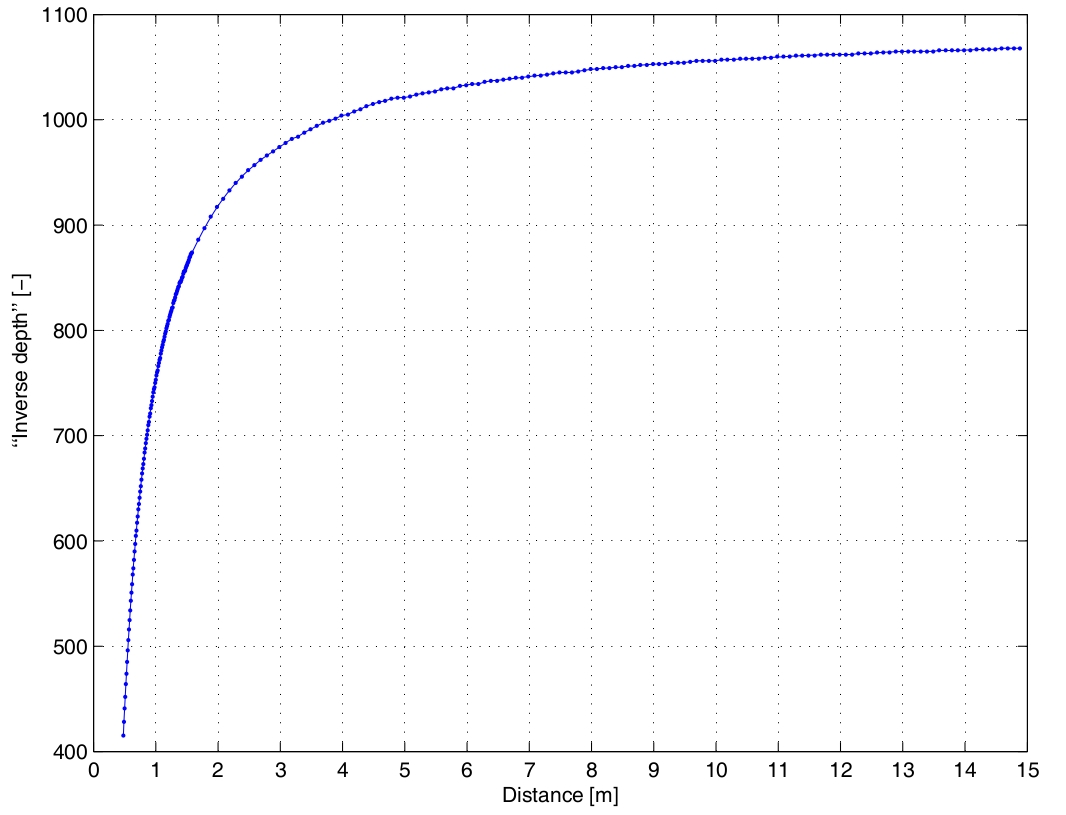
\includegraphics[width=0.6\linewidth,natwidth=640,natheight=640]
  {fig/ref_imgs/depth_disparity_relation.png}
  \caption[Relationship Between Inverse Depth and Disparity]{Non-linear 
  Relationship Between Inverse Depth and Disparity \parencite{Smisek2011}}
	\label{fig:depth_disparity_relation}
\end{figure}

Thus, we need to update depth equation \eqref{eq:depth_wo_disparity} by taking 
its inverse and introducing normalization factor replacing with $d$ with 
$md'+n$:

\begin{equation}\label{eq:depth_w_disparity_reverse}
  {Z^{\mathcal{C}}}^{-1} = (\frac{m}{fb})d' + (Z_r^{-1} + \frac{n}{fb})
\end{equation}

To make it convenient to calculate, we can take its inverse again:

\begin{equation}\label{eq:depth_w_disparity}
  Z^{\mathcal{C}} = \frac{1}{(\frac{m}{fb})d' + (Z_r^{-1} + \frac{n}{fb})}
\end{equation}

The relationship between disparity data and metric depth measurement can be 
written as a function in the following form:

\begin{equation}\label{eq:ir_cam_proj_func}
  Z^{\mathcal{C}}
  =
  F_d(d')
\end{equation} 


Now that we know how to get metric depth information $Z^{\mathcal{C}}$ from 
disparity data 
by utilizing the triangulation model, we can briefly write down similar 
projection operation for the IR camera.

\begin{equation}\label{eq:ir_cam_proj_func}
  \mathbf{u} 
  =
  %Z_i (\mathbf{P_{IR}^{-1}}\mathbf{u}) = 
  \mathbf{K_{IR}} \mathbf{F_d} ({\mathbf{T_{IR}}}_{\mathcal{W}, \mathcal{C}}  
  \mathbf{X^{\mathcal{W}}})
\end{equation} 


Keep in mind that we also need to calibrate the IR camera's intrinsic and 
extrinsic parameters to find related depth related parameters, i.e., 
$f,b,Z_r,m, n$. In the following section, we will discuss how calibration 
processes are performed for an RGB-D camera to measure quality data.

\section{RGB-D Camera Calibration} \label{sb_sc_rgb_calibration}

The calibration process is a crucial part of any computer vision applications, 
and there are many sophisticated techniques to achieve accurate results.  
However, 
it is important to note that full derivations of the calibration formulation 
are not provided in this thesis. Instead, only the important points are 
given.  
Therefore, I refer readers to \parencite{Zhang2000a}, \parencite{Smisek2011}, 
\parencite{Karan2015} and \parencite{Herrera2016a} for the details of an RGB-D 
camera 
calibration.  Since we are about to perform 3 calibration operations: RGB 
camera, IR camera, and depth measurement, we assume that both the RGB and IR 
camera's image planes are aligned for simplicity (in practice, one must 
  perform transformation $\mathbf{T}_{RGB,IR}$ between an RGB 
and IR camera if a feature from the RGB camera used in the IR camera) and they 
have 
1:1 pixel correspondences. Under these assumptions, let's start with the RGB 
and 
IR camera.

\subsubsection{RGB and IR Camera Calibration}

We calibrate the RGB and IR camera since they both project 3D space to 2D 
space, 
but only measuring the different light spectrum. Thus, the calibration process 
for the RGB camera which we will discuss in this section applies for the IR 
camera as well.  To 
begin with, the simplest case which can help us to understand the calibration 
process is that we assume that we know the exact position of 3D points 
$\mathbf{X}^{(\mathcal{W}, 1:m)}$ in 
world coordinate system and exact position of 2D points $\mathbf{u}^{(1:m)}$ 
on 
the image plane.  
One can build a constraint between them by exploiting the projection function:

\begin{equation}
  \mathbf{u_{RGB}}^{(i)} = 
  \begin{pmatrix}
    u^{(i)}\\
    v^{(i)}\\
    1
  \end{pmatrix}
  =
  \mathbf{P_{RGB}}\mathbf{X^{\mathcal{W}}} = 
  \begin{bmatrix}
    p_{00} & p_{01} & p_{02} & p_{03}\\
    p_{10} & p_{11} & p_{12} & p_{13}\\
    p_{20} & p_{21} & p_{22} & p_{23}
  \end{bmatrix}
  \begin{pmatrix}
    X^{(\mathcal{W}, i)}\\
    Y^{(\mathcal{W}, i)}\\
    Z^{(\mathcal{W}, i)}\\
  \end{pmatrix}\label{eq:proj_matrix}
\end{equation} 

Let's now distribute the projection matrix onto the 3D point measurement to 
retrieve individual pixel coordinates:

\begin{equation}\label{eq:u_i}
  u^{(i)} = 
  \frac
  {p_{00}X^{(\mathcal{W}, i)} + p_{01}Y^{(\mathcal{W}, i)} + 
  p_{02}Z^{(\mathcal{W}, i)} + p_{03}}
  {p_{20}X^{(\mathcal{W}, i)} + p_{21}Y^{(\mathcal{W}, i)} + 
  p_{22}Z^{(\mathcal{W}, i)} + p_{23}}
\end{equation} 

\begin{equation}\label{eq:v_i}
  v^{(i)} = 
  \frac
  {p_{10}X^{(\mathcal{W}, i)} + p_{11}Y^{(\mathcal{W}, i)} + 
  p_{12}Z^{(\mathcal{W}, i)} + p_{13}}
  {p_{20}X^{(\mathcal{W}, i)} + p_{21}Y^{(\mathcal{W}, i)} + 
  p_{22}Z^{(\mathcal{W}, i)} + p_{23}}
\end{equation} 


Since $\mathbf{u}^{(1:m)}$ and $\mathbf{X}^{(\mathcal{W}, 1:m)}$ are known, we 
can 
find 
elements of the 
$\mathbf{p} = (p_{00}, p_{01}, \dots, p_{23})^\top$ matrix by solving 
$\mathbf{Ap=0}$ linear system of equations from \eqref{eq:u_i} and 
\eqref{eq:v_i}.  
For a \textit{minimal solution} of this linear system of equations, we need at 
least $n \geq 6$ measurement points to solve the problem because the 
$\mathbf{P_{RGB}}$ matrix has 12 unknowns (11 if the scale is ignored).  Note 
that 
this accounts for having noise-free measurements which does not hold in 
reality. Then, the problem becomes \textit{over-determined}.

\begin{figure}[H]
%\begin{tabular}{cc}
\centering
\subcaptionbox{RGB Images}{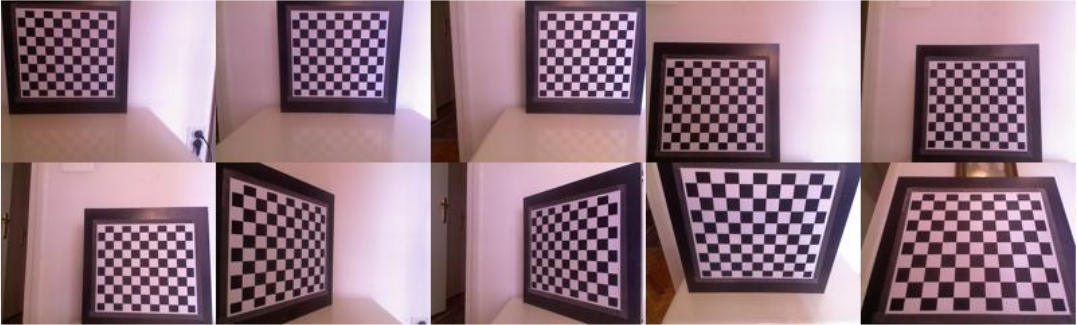
\includegraphics[width = 0.8\linewidth]{fig/ref_imgs/checkerboard_rgb.png}} \\
\subcaptionbox{IR Images}{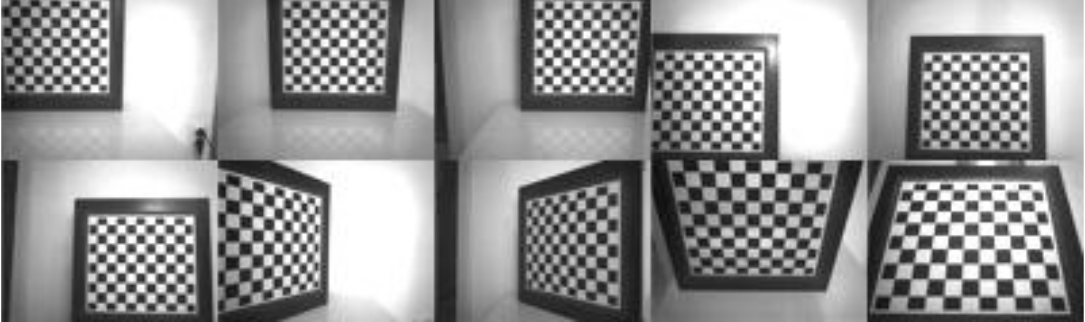
\includegraphics[width = 
0.8\linewidth]{fig/ref_imgs/checkerboard_ir.png}}
%\end{tabular}
\caption[Checkboard Calibration for RGB and IR Camera]{When calibrating RGB 
and IR camera with a checkerboard, one should produce many measurement points 
by placing checker board at different orientation and different tilted 
posture \parencite{Karan2015}.}
\label{fig:checkerboard_rgb_ir}
\end{figure}


In the noisy measurement case, the problem is usually solved with 
\textit{singular 
value decomposition (SVD)} with $n > 6$ measurement points.  This method is 
called the \textit{Direct Linear Transformation (DLT)}. A disadvantage of the 
DLT methods, it is still sensitive errors since it only considers algebraic 
errors (that are the residuals of $\mathbf{Ap}$).  Another drawback of DLT is 
that it cannot compensate non-linearities of projection function due to the 
radial distortions.  Thus, instead of DLT, the non-linear least squares 
optimization is usually performed for better accuracy:

In practice, the checkerboard (see Figure \ref{fig:checkerboard_rgb_ir}) 
is 
used to get many good measurement points as 
we can easily extract edge features from the image as 2D points.  In addition, 
we know the corresponding 3D positions in the world coordinate system.
Also, we have prior knowledge about some of the parameters of intrinsic 
matrix, e.g., pixels are squared, the skew factor is trivial, optical center 
near 
the center of the image. All of these can increase our chance for a successful 
convergence when optimizing:

\begin{equation}\label{eq:proj_lsq}
  \mathbf{x^*}
  = 
  \argmin_{\mathbf{F_{dp}} \rightarrow 
  	\underbrace{
  		\mathbf{K_{RGB}}, 
  \kappa_{RGB}, 
  {\mathbf{T_{RGB}}}_{\mathcal{W}, \mathcal{C}}
  }_{\mathbf{x}}
  }
  \sum_{i=1:n} || \mathbf{u_{RGB}}^{(i)} - 
  \mathbf{F_{dp}} (\mathbf{X}^{(\mathcal{W}, i)}) ||^2
\end{equation}

where $\mathbf{F_{dp}}$ is the projection function along with distortion (see 
notation \eqref{eq:simplyfied_dist_proj_func}), $\mathbf{u}^{(i)}$ is the 
measured pixel coordinates of a feature on the image plane and 
$\mathbf{X}^{(\mathcal{W},i)}$ is the 3D coordinates of a feature in world 
coordinate 
system to identify the following parameters:

\begin{itemize}
  \item $\mathbf{K_{RGB}}$ is the intrinsic matrix for the RGB camera, 
  \item $\kappa_{RGB}$ is the distortion coefficients for the RGB camera, 
  \item ${\mathbf{T_{RGB}}}_{\mathcal{W}, \mathcal{C}}$ is the corresponding 
  transformation from the world coordinate system to the camera coordinate 
  system for the RGB camera.
\end{itemize}

As mentioned earlier, we can apply the same optimization process for the IR 
camera 
to find $\mathbf{K_{IR}}$ intrinsic matrix, $\kappa_{IR}$ 
distortion coefficients and ${\mathbf{T_{IR}}}_{\mathcal{W}, 
	\mathcal{C}}$ corresponding transformation for the IR camera.


\subsubsection{Depth Measurement Calibration}

As we discussed in the previous section, disparity data for every pixel on the 
IR 
image corresponds to the metric depth information.  We can only build the 
relationship between pixel coordinates of the IR image and disparity value 
when the IR camera is calibrated.

\begin{figure}[H]
	\centering
  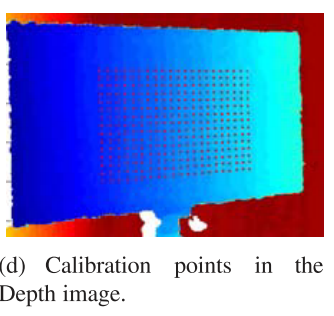
\includegraphics[width=0.7\linewidth,natwidth=640,natheight=640]
  {fig/ref_imgs/checkerboard_depth.png}
  \caption[Checkboard Calibration for Depth]{When calibrating the depth 
  parameters, checkerboard should be placed at different distances to the 
  camera so that we get enough measurement points, especially for fitting 
  $m,n$ parameters \parencite{Karan2015}.}
  \label{fig:checkerboard_depth}
\end{figure}

To get the disparity for $i^{th}$ feature point, a simple mask function can be 
used:

\begin{equation}
  d'^{(i)} = M(\mathbf{u_{IR}}^{(i)})
\end{equation}

where $M$ is a function that return the disparity value at pixel coordinates 
$\mathbf{u_{IR}}^{(i)}=(u_{IR}^{(i)},u_{IR}^{(i)})^\top$ of calibrated IR 
image.  
Then, our one last step will be to convert disparity measurement to depth for 
every feature on the checkerboard and minimize the error between measured 
depth 
$\hat{Z^{\mathcal{C}}}=F_d(d')$ (see notation \eqref{eq:ir_cam_proj_func}) and 
real depth 
$Z^{\mathcal{C}}$:

\begin{equation}\label{eq:proj_lsq}
  \mathbf{x^*} = 
  \argmin_{F_d \rightarrow \underbrace{f, b, Z_r, m, n}_{\mathbf{x}}}
  \sum_{i=1:n} || Z^{(\mathcal{C}, i)} - F_d(d'^{(i)})  ||^2
\end{equation}

The calibration processes for cameras are a well-studied problem in the 
computer 
vision literature.  Fortunately, there are many open software libraries, such 
as OpenCV, that offers such implementations.

In summary, this chapter gave both a theoretical and practical background 
for an RGB-D camera. The first and most important topic was the pinhole 
camera model that simplifies the working principles of a projective camera. 
As discussed, we lose depth information during projection operation. Hence, 
we studied the triangulation method that retrieves the metric depth 
with the Structured-Light IR speckles. Lastly, the calibration techniques of 
an RGB-D camera were given. In the following chapter, we will dive more 
into the algorithmic part of VO.

\chapter{Fundamentals of Visual Odometry} \label{cp_vo}

\section{Related Work} \label{sc_visual_odometry_related_works}

% What is VO?
As being part of dead-reckoning systems, VO provides the \textit{ego-motion}
estimation of an agent by exploiting only one or multiple cameras. The working
principle of VO relies on the following idea: if we had two subsequent images
captured by the camera in a 3D space, it would tell us about a change in the 
camera's
pose from one image to another as changing patterns of objects' shapes or
pixels' intensity occurs during motion.  This change in the pose refers as
\textit{relative pose} which we want to know ultimately.

% First ego motion estimation with cam
% - Moravec1980 - Obstacle Avoidance and Navigatio n in the Real World by a Seeing Robot Rover
% - Matthies1987a - Error Modeling in Stereo Navigation
% - Olson2003 - Rover navigation using stereo ego-motion
First research in estimating camera ego-motion was done in a Ph.D. thesis 
\parencite{Moravec1980} in the 1980s. He used a sliding camera as a stereo 
fashion 
that captures images when the robot stops after moving for some small 
distance. Another early study, from  
\parencite{Matthies1987a}, 
formulated the ego-motion estimation for stereo vision. The interest in VO 
peaked after NASA's Mars expeditions with a rover in 2003. Therefore, 
researchers and 
engineers in NASA JPL further improved the robustness of their mobile robots 
with the VO system \parencite{Olson2003}.
% First VO Paper
% Nister2004 - Visual Odometry

In computer vision, Structure from Motion (SFM), that tackles 3D 
reconstruction of an environment with moving camera, is a well-studied topic. 
For SFM, it is critical to estimate camera pose accurately if one wants to 
build the 3D 
environment. On the other hand, VO can be thought of a subset problem of SFM. 
The reason VO 
parted 
from SFM is that VO systems started to empower other applications such as SLAM 
and are required to operate in real-time, all of which introduces a great 
challenge.

% Surveys
% - Fraundorfer2012 - Visual odometry: Part I: The First 30 Years and 
%Fundamentals
% - Scaramuzza2011 - Visual Odometry Part II: Matching,Robustness, 
%Optimization, and Applications
% - Aqel2016 - Review of visual odometry: types, approaches, challenges, and 
%applications
For the first time, Visual Odometry term was introduced in 
\parencite{Nister2004}. 
It estimates the transformation matrix by solving the P3P problem between 
consecutive frames. \cite{Nister2004} also demonstrated a VO pipeline that 
became a 
defacto system configuration even for today's VO applications. With the help 
of early robotics applications in NASA and the computer vision community, the 
VO 
became a quite popular field. That being said, two of the most influential 
papers were \parencite{Fraundorfer2012} and \parencite{Scaramuzza2011}. By 
publishing 
these tutorials, the authors gave researchers and engineers a 
design recipe 
for building the VO system for different kind of environment settings since 
there is no such a system that works under any conditions. Additionally, one 
can find a 
survey of VO types, approaches and challenges in \parencite{Aqel2016}.

Over the years, research on VO is progressively increased and various types of 
VO systems are proposed. Therefore, VO systems can be categorized based on 
different phenomena such as camera sensor types and solver algorithms choice. 
As for the camera choice, One can utilize monocular or stereo cameras to 
capture images. The stereo 
cameras are further grouped into two categories; i.e., active and passive 
cameras. For the active camera, besides color or monochrome camera, there is 
another camera such IR camera that helps to measure the depth information 
combination 
with IR laser projector. For the passive camera, the depth is calculated from 
two color or a monochrome camera. 

As for the solver algorithms, one can 
group VO into two categories; i.e., feature-based and appearance-based.
The feature-based VO algorithms are interested in extracting distinct and 
repeatable feature points from images and finding correspondences in extracted 
features either between consecutive frames or keyframes. The challenging part 
in feature-based VO is to build a system that can match features across 
different frames without errors. However, this does not hold in reality, so 
one typically needs to remove these errors with outlier rejection algorithms 
such as RANSAC \parencite{Fischler1981b}. Among many VO systems, there are two 
favorite open source feature-based VO tools which stand out; i.e., LIBVISO2 
\parencite{Geiger2011} and FOVIS \parencite{Huanga2011}. 

Briefly, LIBVISO2 uses both 
simple blob and corner filters to extract features. The extracted features are 
filtered by non-maximum suppression to increase the robustness of the matching 
process. Then, it calculates the depth information by triangulation technique 
as it uses a passive stereo camera. Finally, it minimizes the reprojection 
error. The reprojection error function is constructed by projection from 
features on the left camera onto the right camera and vice-versa, to estimate 
the pose. Note that RANSAC applied on feature matches to remove outliers. 

Whereas, FOVIS is more accurate and faster than LIBVISO2 according to 
\parencite{Fang2015a}.
% RGBD VO Comparisons
%% - Angladon2017 - An evaluation of real-time RGB-D visual odometry algorithms on mobile devices
% - Fang2015a - Experimental evaluation of RGB-D visual odometry methods
FOVIS uses only FAST corner detectors to extract features. For matching 
features, it takes advantage of keyframes instead of consecutive images to 
reduce the drift effect. Instead of using RANSAC for outlier rejection, it 
constructs 
a graph of consistent feature matches and updates the features that obey the 
following idea: the Euclidean distance between two features at one time should 
match 
their distance at another time. Finally, several refinement processes are 
applied during motion estimation to improve accuracy.
% RGBD VO Implementations
% - Geiger2011 - LIBVISO2 - StereoScan: Dense 3d Reconstruction in Real-time
% - Huanga2011 - FOVIS - Visual Odometry and Mapping for Autonomous Flight Using an RGB-D Camera

The most significant disadvantage of feature-based VO is that the accuracy of 
the pose estimations decreases if the operating environment lacks texture-rich 
scenes such as corridors or the measured images are blurry due to fast 
motions. Thus, appearance-based VO algorithms utilize the entire image instead 
of extracted features. Initially, Iterative Closest Point (ICP) 
\parencite{Besl1992} was used to minimize the geometrical error between 3D 
surfaces. Then, various kinds of ICP algorithms are built for improving 
efficiency \parencite{Rusinkiewicz2001}. Even though ICP is useful for 
creating 
3D 
shapes with point clouds, it is slower and less accurate compared to 
feature-based methods.
% - Besl1992 - First ICP Paper - A method for registration of 3-D shapes
% - Rusinkiewicz2001 - ICP - Efficient Variants of the ICP Algorithm
Then, another type of appearance-based approach, so-called Dense Visual 
Odometry (DVO) \parencite{Kerl2013a}, was emerged. Fundamentally, it minimizes 
the 
photometrical 
error based on the pixel intensity between consecutive frames. Although the 
original techniques developed with appearance-based approaches produces less 
accurate results, we can say that it recently started to gain popularity with 
carefully designed hybrid methods, so-called Semi-Dense VO 
\parencite{Zhou2017a}, 
and it can outperform feature-based VO in some cases.
% - Kerl2013a - DVO - Robust Odometry Estimation for RGB-D Cameras

In this chapter, we will focus on the standardized feature-based VO pipeline, 
which will serve us as a foundational basis so that we comprehend the 
algorithmic errors. Hence, we structured this chapter according to four main 
components of the pipeline: (1) feature extraction, (2) feature matching, (3) 
outlier rejection and (4) pose estimation. 


\section{Feature Extraction} \label{sc_feature_extraction}

Image features are a collection of regions of interest or points of interest 
that describe the image. In this way, we compress the necessary information 
from images so that we can deal with computationally expensive image 
processing tasks. Points of interest $\mathbf{u}^{(i)}$, which also can be 
called as 
\textit{key points}, \textit{features} or \textit{landmarks} interchangeably, 
are particularly valuable because their location can be measured 
accurately on an image. This is useful for localization-related tasks such as 
VO. 

In feature-based VO, the critical task is to find good features.  What defines 
good features from others is that they are distinct, repeatable, 
computationally cheap and invariant to geometrical changes. In this regard, 
one has many 
options to produce such image, but two common methods in VO systems are blobs 
and corners. Blobs are image patterns that contain distinct image response 
comparing to their neighborhood pixels. they take advantage of pixel 
intensity or color to decide whether it has a distinct response or not.  In 
the VO literature, SIFT \parencite{Lowe2004} and SURF \parencite{Bay2008} are 
popular 
choices for detecting blob features.  In contrast, corners are the meeting 
points where two or many edges intersect.  they exploit the 
geometrical structure of an image.  FAST \parencite{Rosten2006} and Harris 
\parencite{Harris1988} are widely used for detecting corners.

Fundamentally, a two-step process is needed to extract good features.  In the 
first step, 
you take a response function called \textit{image filter}, shift this filter 
through the image and save the one that has a greater response than your 
previously defined threshold.  This might be a Gaussian filter for blobs or a 
corner detector filter for corners. In the second step, you perform non-maxima 
suppression on the resulting image features to find local minima of the 
function.  This step will help to remove similar image features and to choose 
the ones having maximum confidence so that distinctiveness of the features are 
ensured.  Note that some VO might skip non-maxima suppression because of the 
efficiency 
reasons.

Inherently, each feature detector has certain limitations, and one has to 
choose which detector to use depending on task objectives. Therefore, we may 
ask the following question: Does the localization environment involve more 
texture-oriented objects like floors, walls, etc. or geometrical shapes like 
urban areas where many lines exist?  However, the rule of thumb is that blobs 
are distinct but slow to compute and corners are fast to compute but less 
distinct according to \parencite{Fraundorfer2012}. 

After extracting features, one needs to encode the detected image features 
into a format that we can perform comparison operations among them. 
This encoding is done by taking the neighboring pixels around the image 
features and 
convert into a more compact form. For example, SIFT (1) creates a patch around 
an 
image feature, (2) divides this patch into 
smaller grids, (3) calculate the gradient of each grid and (4) saves them as a 
histogram.  This procedure makes feature descriptor robust against scale or 
rotation changes. Then, one can use these descriptors for comparison 
operations such as matching or tracking in VO. 

In this thesis, we utilize ORB (Oriented FAST and Rotated BRIEF). ORB offers 
both the feature extraction and description capability. The feature 
extraction is done by FAST corners. Then, the extracted FAST corners are 
ranked with Harris based on their image derivatives so that one can select 
top N corners with greater distinction. After extracting features, the 
feature descriptors are formed with BRIEF to encode necessary pixel 
information around the extracted feature. To feature descriptors, BRIEF takes 
a patch $\mathbf{S}$ around the extracted features and performs binary 
comparisons between randomly selected pixels in $\mathbf{S}$. 
However, BRIEF is not robust against rotations so ORB rotates BRIEF 
descriptors with the calculated corners' angle. In short, although the overall 
accuracy 
of SIFT is better than ORB, we choose ORB because it is faster and more than 
SIFT. For more details on how to extract ORB features, I refer readers to 
Appendices \ref{sb_sc_orb}.


\section{Feature Matching} \label{sc_feature_matching}

Typically, a camera can procedure a video stream consisting of 
usually ranging from 30 to 60 frames per second. 
Now that we know how to extract a feature and form a descriptor, 
we can start building a relationship across frames with feature descriptors to 
estimate how a camera 
moves. 
Therefore, the second task in VO after 
extracting features is to form a group of image pairs information between each 
image pair, continuously. In literature, there are two ways to select image 
pairs: frame to frame or keyframe to frame. In the former case, one groups 
consecutive frames across video stream. In the latter case, one selects a 
reference frame and keep matching it with subsequent frames as long as the 
pair has a sufficient amount of feature matchings. The latter has certain 
advantages over the former; however, we choose the former as we wish to model 
the uncertainty of our motion estimation algorithm as accurate as possible. 

\begin{figure}[H]
	\centering
	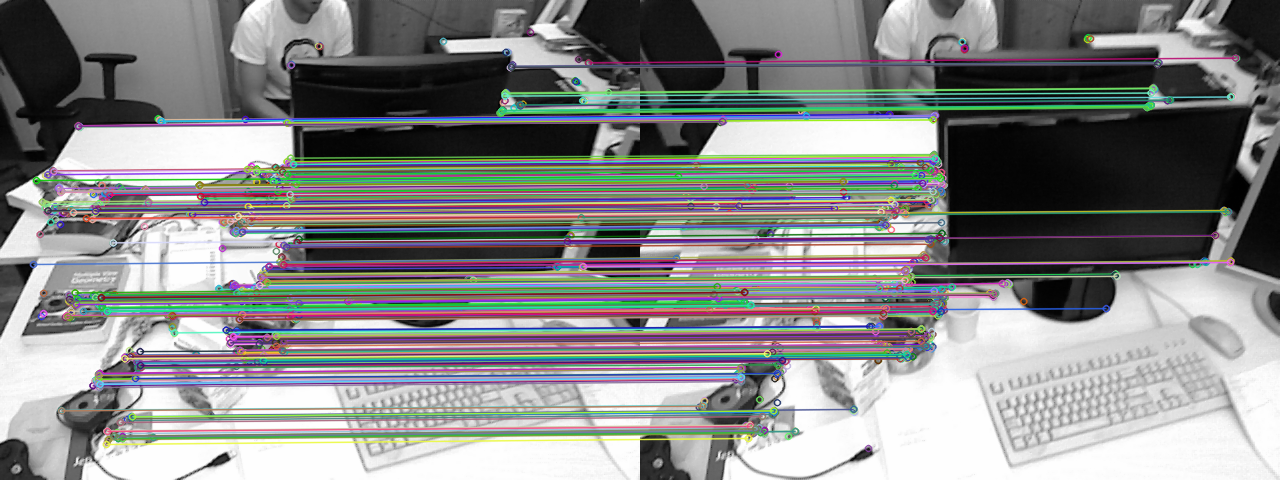
\includegraphics[width=\linewidth,natwidth=640,natheight=640]
	{fig/ref_imgs/covo_matches.png}
	\caption[ORB Feature Mathces]
	{An example feature matching scene from 
	TUM RGB-D (freiburg xyz) dataset with ORB.}
	\label{fig:feature_matchings}
\end{figure}

Having said that let's assume we pair consecutive images $(\mathbf{I}^{(k)}, 
\mathbf{I}^{(k+1)})$. In each image, we gather feature descriptors 
$(\mathbf{D}^{(k,1:n)}, \mathbf{D}^{(k+1,1:m)})$ that pass through our ORB 
filter. The goal is to find the feature correspondences based on their rotated 
BRIEF descriptor values. Again, there are many efficient ways to perform this 
matching task such as FLANN (Fast Library for Approximate Nearest Neighbors). 
Instead, in this thesis, we choose the Brute-Force matching algorithm.
Even though which it is less efficient in terms of time complexity, it 
produces fewer outliers. This is especially important for us as we aim for as 
minimum outliers as possible for our VO so that we can model the uncertainty 
accurately. 
In short, the Brute-Force, as its name states, is a straightforward technique 
that 
compares each $\mathbf{D}^{(k,1:n)}$ descriptors in $k^{th}$ image with 
$\mathbf{D}^{(k+1,1:m)}$ descriptors in $k+1^{th}$ image by calculating 
\textit{Hamming} distance to each other:

\begin{equation}
  d_h(\mathbf{D}^{(k,i)},\mathbf{D}^{(k+1,j)}) = \mathbf{D}^{(k,i)} \oplus 
  \mathbf{D}^{(k+1, j)}
\end{equation}

where $\oplus$ corresponds to an 'exclusive or' logic operation. Then, if the 
distance is greater than the specified threshold, we call it a match. 
Additionally, we perform a cross-check validation by ensuring that matches 
with value $(i,j)$ such that $i^{th}$ descriptor in image $k$ has $j^{th}$ 
descriptor in image $k+1$ as the best match and vice-versa.
Note that we still keep the Hamming distance information with their 
corresponding matches so that we can select top N matches, after 
determining matches.


\section{Outlier Rejection} \label{sb_sc_ransac}

In reality, not all feature matches are correct, and it is critical that we 
detect wrong ones as the optimization algorithm that estimates the camera 
motion is sensitive to even a small number of wrong matches. In technical 
terms, we call these wrong matches \textit{outliers} (or \textit{false 
positives}). Hence, we need an algorithm to reject those outliers from 
\textit{inliers} (or \textit{true positives}). 

The most common way is to utilize 
RANSAC 
\parencite{Fischler1981b} algorithm, 
which is an abbreviation to Random Sample Consensus. In short, RANSAC is an 
iterative 
algorithm which fits the desired model with the presence of outliers by 
selecting a subset of dataset randomly and improving parameters of model each 
iteration. Note that RANSAC works well if at least half of the dataset 
contains inliers. Since outliers plays a big part of modeling a metric 
uncertainty of features accurately, I refer readers to Appendices 
\ref{sb_sc_ransac_app} 
where we discuss details of the RANSAC algorithm. 


It is crucial to note that we may still have outliers after RANSAC.  However, 
our motion estimation will be greatly improved since the majority of the 
outliers are removed.  Finally, we will discuss how we can utilize the 
carefully selected features and its matches to estimate the camera motion. 


\section{Pose Estimation} \label{sc_pose_estimation}

Pose estimation is the core part of the VO system. After extracting and 
matching features, we finally are ready to compute \textit{transformation} 
information. The transformation corresponds to relative camera motion between 
two images that are recorded in different poses (see 
figure-\ref{fig:transformation_ij}). Let's assume; we have consecutive camera 
poses $\mathbf{x}_{k}^{\mathcal{C}} = [\mathbf{p}_k^{\mathcal{C}}, 
\mathbf{q}_k^{\mathcal{C}}]^\top$ and 
$\mathbf{x}_{k+1}^{\mathcal{C}} = 
[\mathbf{p}_{k+1}^{\mathcal{C}}, \mathbf{q}_{k+1}^{\mathcal{C}}]^\top$ in 
$SE(3)$ 
where 
$\mathbf{p}^{\mathcal{C}} = [p_x^{\mathcal{C}}, 
p_y^{\mathcal{C}}, p_z^{\mathcal{C}}]^\top$ 
is the position of the camera in $\R^3$ and 
$\mathbf{q}^{\mathcal{C}} = [q_w^{\mathcal{C}}, q_x^{\mathcal{C}}, 
q_y^{\mathcal{C}}, 
q_z^{\mathcal{C}}]^\top$ is the orientation of the camera in quaternion 
form in 
$SO(3)$. Both the position and orientation is measured with respect to the 
camera coordinate system as well.  
Notice that, in camera model Chapter \ref{cp_cam_models}, we use rotation 
matrix to represent orientations, which made it convenient to combine 
intrinsic matrix and extrinsic matrix into a single projection matrix (see 
notation \eqref{eq:simplyfied_proj_func}). On the other hand, when estimating 
relative motion, we use 
quaternions to represent orientations, which is less intuitive but has 
certain advantages over rotation matrix such as requiring less storage.  

In addition, we can represent the transformation 
$\mathbf{x}_{k,k+1}^{\mathcal{C}} 
= 
\mathbf{T}_{k,k+1}^{\mathcal{C}}= 
[\mathbf{t}_{k,k+1}^{\mathcal{C}},\mathbf{q}_{k,k+1}^{\mathcal{C}}]^\top$ 
between 
two camera poses 
$(\mathbf{x}_k^{\mathcal{C}},\mathbf{x}_{k+1}^{\mathcal{C}})$ with the 
translation $\mathbf{t}_{k,k+1}^{\mathcal{C}}$ in $\R^3$ and  
rotation $\mathbf{q}_{k,k+1}^{\mathcal{C}}$ in $SO(3)$. 
That being said, 
one can formulate the transformation $\mathbf{T}_{k,k+1}^{\mathcal{C}}$ 
between two camera 
pose if the initial pose $\mathbf{x}_{0}^{\mathcal{C}}$ is known. 
For our convenience, we will drop $\mathcal{C}$ superscript by assuming that 
all transformations are executed in the camera coordinate system. 
Let's first find the next camera position considering the position at $k^{th}$ 
is known:

\begin{equation}\label{eq:translation_cam}
  \mathbf{p}_{k+1} = 
\mathbf{q}_{k,k+1} \otimes \mathbf{p}_k \otimes \mathbf{q}_{k,k+1}^* + 
  \mathbf{t}_{k,k+1}
\end{equation}

where $\mathbf{q}_{k,k+1} \otimes \mathbf{p}_k \otimes \mathbf{q}_{k,k+1}^*$ 
is the \textit{hamilton product} that rotates the camera position at the 
$k^{th}$ pose initially and $\mathbf{t}_{k,k+1}$ is the simple vector addition 
that 
translates the camera position. Next, the camera orientation can be found as 
follows:

\begin{equation}\label{eq:rotation_cam}
  \mathbf{q}_{k+1} = 
  \mathbf{q}_{k,k+1} \otimes \mathbf{q}_{k}
\end{equation}

where $\mathbf{q}_{k,k+1} \otimes \mathbf{q}_{k}$ is the product of two 
quaternions that the former is the rotation of the camera movement and that 
the latter is the 
orientation of the camera at the $k^{th}$ pose. For more detailed formulation 
and better visualization for rigid-body transformations, I refer readers to 
Appendices \ref{sc_rigid_body_transformations}.

\begin{figure}[H]
	\centering
  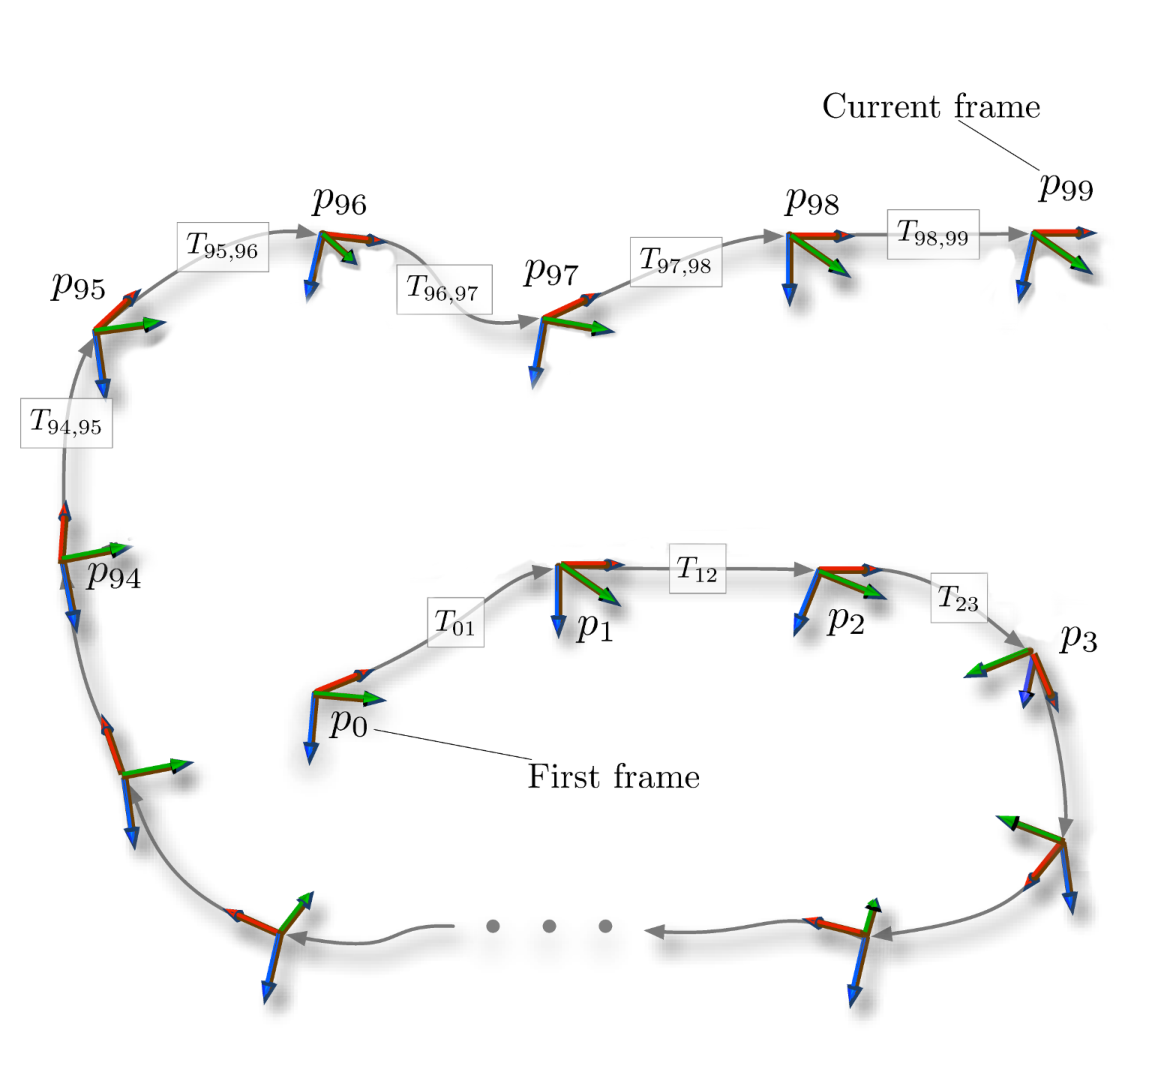
\includegraphics[width=0.7\linewidth,natwidth=640,natheight=640]
  {fig/drawings/rel_pose.pdf}
  \caption[Trajectory From Relative Pose]
  {VO estimates the ego-motion of the camera by relative poses estimated from  
  image pairs. Thus, it assumes that the initial pose $\mathbf{x}_0$ of the 
  camera is 
  known. Transformation $T_{0,1}$ from one image to another corresponds to the 
  camera movement from one position to another. As long as VO is able to 
  detect a sufficient number of features, it keeps estimating relative 
  transformations. With all of these transformations, one can build a 
  trajectory $(T_{0,1}, \dots, T_{98,99})$ which the camera follows.}
	\label{fig:transformation_ij}
\end{figure}

The ultimate goal in VO is to compute transformation 
$\mathbf{x}_{k,k+1}(=\mathbf{T}_{k,k+1})$ in 
multiple consecutive images and concatenate them to build a trajectory of the 
camera. As a consequence, we can track any agent on which the camera is placed 
rigidly. For example, concatenated transformation 
$\mathbf{x}_{0:n}(=\mathbf{T}_{0:n})$ can be 
used to calculate $n^{th}$ camera pose that is relative to the initial pose:

\begin{equation}
  \mathbf{p}_{n} = 
  \mathbf{q}_{n, n-1} \otimes (\dots
  (\mathbf{q}_{2,1} \otimes
  (\mathbf{q}_{1,0} \otimes \mathbf{p}_0 \otimes \mathbf{q_{1,0}}^* + \mathbf{t}_{1,0})
  \otimes \mathbf{q}_{2,1}^* + \mathbf{t}_{2,1})
  \dots) \otimes \mathbf{q}_{n, n-1}^* +\mathbf{t}_{n, n-1} 
\end{equation}

\begin{equation}
  \mathbf{q}_{n} = 
  \mathbf{q}_{n,n-1} \otimes \dots \otimes \mathbf{q}_{2,1} \otimes \mathbf{q}_{1,0} \otimes \mathbf{q}_{0} 
\end{equation}

To find transformation, we take advantage of image features as they can inform 
us how the camera moves if we detect them across multiple frames.  All the 
aforementioned steps such as feature extraction and feature matchings are 
performed for the purpose of computing relative motion. Similar to the 
projection 
matrix in camera calibration, we utilize the least squares 
method for estimating an approximated transformation information due to the 
noise. 

%\subsection{Relative Pose Estimation Techniques}
%\label{sb_sc_relative_camera_pose_estimation_techniques}

So far, we discussed how we could process images so that we have adequate 
information to compute camera pose. However, we only mentioned 2D image 
features. To estimate the pose in the 3D world, we require corresponding depth 
information for features. Note that there are methods that retrieve relative 
scale information using only 2D image features and its epipolar constraints 
with monocular cameras, but we are interested in having metric depth 
information rather than relative scale in this thesis. Therefore, we have two 
common choices regarding camera types: stereo cameras or RGB-D cameras. In our 
experiments, we experimented on an RGB-D camera to retrieve the depth 
information.

At this point, one generally has two ways to compute relative camera poses.  
The reason we have different two different methods to compute transformation 
arises 
from the cost function we define for the least squares problem. In the end, 
all we wish to find a good model for our optimization problem so that we 
settle on the best possible local minimum.  The design choice for cost 
function comes from the fact that we build our cost function either on $\R^2$ 
space (image plane) or $\R^3$ space (camera coordinate system).  Therefore, in 
VO literature, there are two different cost functions for modeling the least 
problem:

\begin{itemize}
  \item 3D-to-2D correspondences,
  \item 3D-to-3D correspondences.
\end{itemize}


The 2D term refers to 2D image features. Whereas, the 3D term refers to 3D 
point features.  Note that this thesis does not engage with 2D-to-2D 
correspondences method since it is used in monocular camera; thus it will not 
be discussed here. Although 3D-to-2D 
correspondences outperform 3D-to-3D correspondences in VO, we show that the 
accuracy of 3D-to-3D correspondences can be significantly improved if the 
uncertainty of the 3D point features is modeled properly and used in the 
optimization process.  On the plus side, this technique allows us to propagate 
the uncertainty of the 3D feature points to get the uncertainty of the 
estimated 
pose. Now, let's explain both methods.


\subsubsection{3D-to-2D Correspondences}\label{sb_sc_3d_to_2d}

Remember that, after feature matching step for the consecutive image frames, 
we have only 2D-to-2D correspondences information and the transformation which 
we wish to compute is in $\R^3$. Therefore, we require transformation 
involving in 3D point features. That being said, we can estimate 
transformation 3D-to-2D Correspondences in four steps:

\begin{enumerate}
  \item Back-project 2D image features from $k+1^{th}$ frame to form 3D point features,
  \item Back-transform 3D point features from $k+1^{th}$ frame towards $k^{th}$ frame 
    with the transformation matrix,
  \item Reproject the back-transformed 3D point features onto the $k^{th}$ image plane, 
  \item Minimize 2D Euclidean distance error between reprojected and measured 2D image features.
\end{enumerate}

\begin{figure}[H]
	\centering
  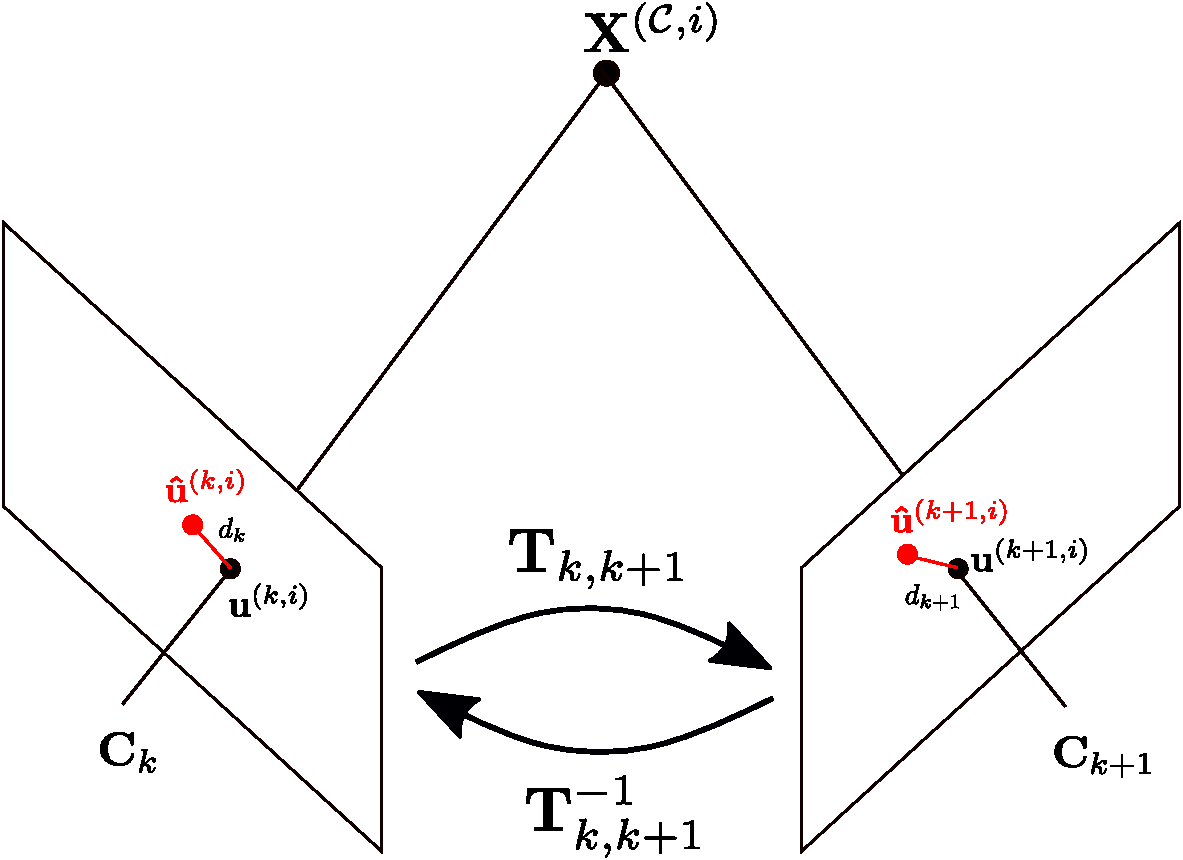
\includegraphics[width=0.9\linewidth,natwidth=640,natheight=640]
  {fig/drawings/3d_to_2d.pdf}
  \caption[3D-to-2D Correspondences]{Assuming that we have two frames taken in 
  the different poses. What 3D-to-2D correspondences method does is that it 
  takes the pixel $\mathbf{u}^{(k+1,i)}$ measurement from $k+1^{th}$ 
  back-projects to get the 3D point feature, then rotates and translates with 
  the transformation information, and projects the 3D feature to the 2D 
  feature as $\mathbf{\hat{u}}^{(k,i)}$ on image plane at $k^{th}$ frame. 
  Afterward, one will get Euclidean error distance $d_k \in \R^2$ between the 
  reprojected pixel and the measured pixel. This behavior applies for 
  reprojection of image features from $k^{th}$ to $k+1^{th}$ frame to 
  calculate $d_{k+1}$. 
  For the sake of efficiency, most VO algorithms assume that measurement 
  errors occur in only one image pair and only uses $d_k$ to minimize the 
  error, but not both $d_k+d_{k+1}$. Note that 
  this choice might decrease the accuracy of the 
  pose estimation.}
	\label{fig:min_geometric_error}
\end{figure}


To formulate the problem more clearly, let's assume we have a 3D point feature 
$\mathbf{X}^{(\mathcal{C}, i)}$ in camera coordinate system and 
we measure 
the projections of this exact feature point as a 2D image feature, 
$\mathbf{u}^{(k,i)}$ and $\mathbf{u}^{(k+1,i)}$ on subsequent 
camera poses $k^{th}$ and $k+1^{th}$ respectively. What we also know is that 
we can back-project measured 2D image features as 3D point features using 
the projection matrix (see notation \eqref{eq:simplyfied_proj_func_1}) and 
depth 
information. Let's write again projection function that converts 3D point 
features to 2D image features: $\mathbf{u}^{(k,i)} = 
\mathbf{K}\mathbf{X}^{(k,i)}$ and $\mathbf{u}^{(k+1,i)} = 
\mathbf{K}\mathbf{X}^{(k+1,i)}$.
One can also back-project 2D image features to 3D point features: 
$\mathbf{X}^{(k,i)} = \mathbf{K}^\top \mathbf{u}^{(k,i)}$ and 
$\mathbf{X}^{(k+1,i)} = \mathbf{K}^\top \mathbf{u}^{(k+1,i)}$. 
After back-projecting 2D image features to 3D point features, 
we get two 
$(\mathbf{X}^{(k,i)},\mathbf{X}^{(k+1,i)})$ measurements with respect to the 
$k^{th}$
and $k+1^{th}$ frame for  
same $\mathbf{X}^{(\mathcal{C}, i)}$ point feature in the camera coordinate 
system. 
Now, we can formulate the 
previously discussed four steps of 3D-to-2D correspondences as follows:

\begin{enumerate}
  \item $\mathbf{X}^{(k+1,i)} = \mathbf{K}^\top \mathbf{u}^{(k+1,i)}$
  \item $\mathbf{\hat{X}}^{(k,i)} = f(\mathbf{t}_{k,k+1}, \mathbf{q}_{k,k+1}, 
  \mathbf{X}^{(k+1,i)}) = 
    \mathbf{q}_{k,k+1} \otimes \mathbf{X}^{(k+1,i)} \otimes 
    \mathbf{q}_{k,k+1}^* + \mathbf{t}_{k,k+1} $
  \item $\mathbf{\hat{u}}^{(k,i)} = \mathbf{K}\mathbf{\hat{X}}^{(k,i)}$
  \item minimize $\sum_i||\mathbf{u}^{(k,i)} - \mathbf{\hat{u}}^{(k,i)}||^2$ 
  where 
    $\mathbf{u}^{(k,i)}$, $\mathbf{\hat{u}}^{(k,i)} \in \R^2$
\end{enumerate}

The second and third steps can be encapsulated to a function $f$ so that 
we form the problem as an optimization problem in the following form:

\begin{equation}
  \mathbf{x^*}_{k,k+1} = \argmin_{\mathbf{x}_{k,k+1} = [\mathbf{t}_{k,k+1}, 
  \mathbf{q}_{k,k+1}]}
  \sum_i||\mathbf{u}^{(k,i)} - f(\mathbf{t}_{k,k+1}, \mathbf{q}_{k,k+1}, 
  \mathbf{X}^{(k+1,i)})||^2
\end{equation}


\subsubsection{3D-to-3D Correspondences}\label{sb_sc_3d_to_3d}

Another way of modeling the cost function is to utilize only 3D point features 
correspondences. One can estimate transformation with 3D-to-3D 
correspondences in three steps:

\begin{enumerate}
  \item Back-project both 2D image features from $k^{th}$ and $k+1^{th}$ 
  frames as 3D point features, 
  \item Back-transform the back-projected 3D point features from $k+1^{th}$ 
  frame,
  \item Minimize 3D Euclidean error distance between back-transformed and 
  measured 3D point features.
\end{enumerate}

\begin{figure}[H]
	\centering
	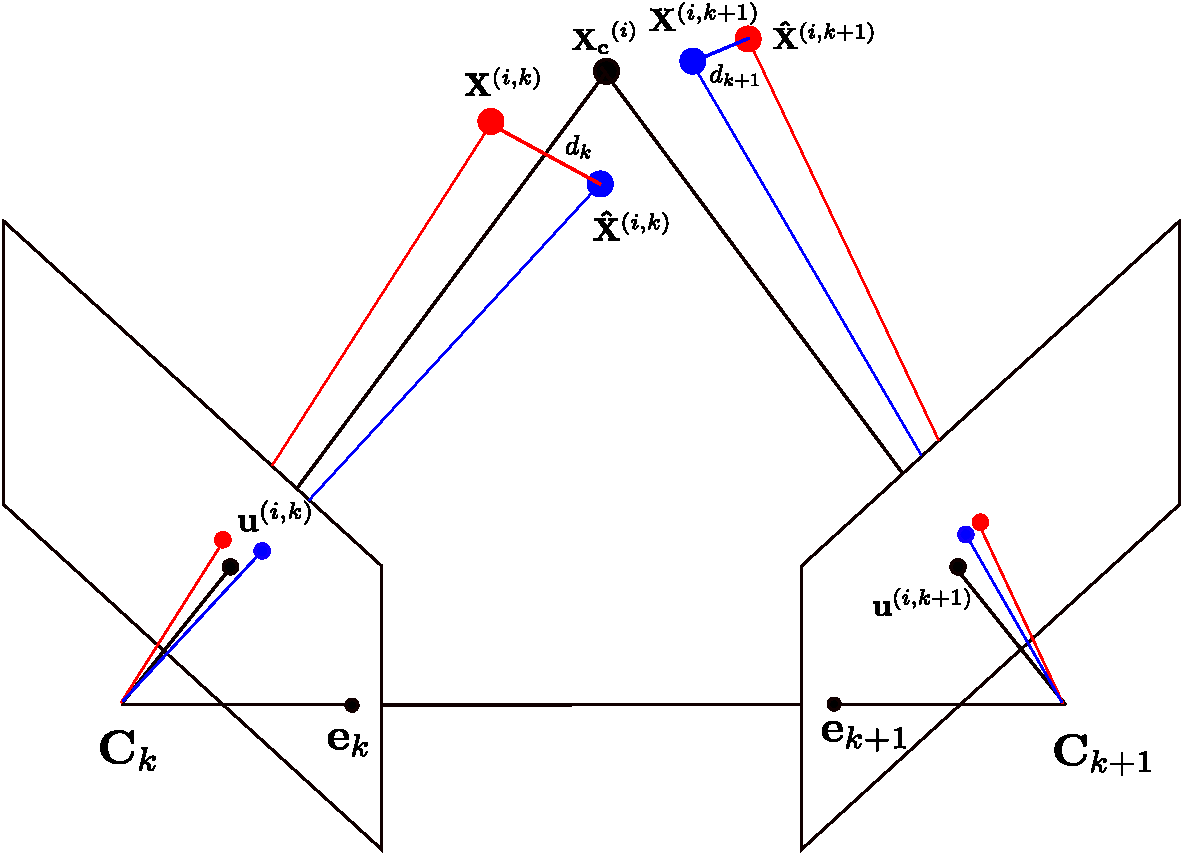
\includegraphics[width=0.9\linewidth,natwidth=640,natheight=640]
	{fig/drawings/3d_to_3d.pdf}
	\caption[3D-to-3D Correspondences]
	{3D-to-3D correspondences method calculates the Euclidean error distance 
	in 
	3D space. For example, all image features are 
	back-projected to get 3D point features 
	$\mathbf{X}^{(k,i)},\mathbf{X}^{(k+1,i)}$. Then, $\mathbf{X}^{(k+1,i)}$ is 
	rotated and translated with the transformation information 
	$\mathbf{T}_{k,k+1}$ to align the same 3D point feature 
	$\mathbf{\hat{X}}^{(k,i)}$ with respect to $k^{th}$ camera's center. In 
	this 
	way, one can calculate the Euclidean distance error $d_k \in \R^3$. 
	The reverse 
	behavior applies on moving features from $k^{th}$ to $k+1^{th}$ frame to 
	calculate $d_{k+1}$ as well.}
	\label{fig:min_euclidean_error}
\end{figure}


The similar formulation that we previously did for 3D-to-2D correspondences 
applies for the 3D-to-3D correspondences as well but only with few changes. 
Let's again assume that we have two corresponding 2D image features, 
$\mathbf{u}^{(k,i)}$ and $\mathbf{u}^{(k+1,i)}$. However, rather than 
minimizing error on the 2D image plane, we want to minimize them on 3D space. 
Therefore, we need to back-project both image features. With that in mind, we 
can formulate the three steps of 3D-to-3D correspondences as follows:

\begin{enumerate}
  \item $\mathbf{X}^{(k+1,i)} = \mathbf{K}^\top \mathbf{u}^{(k+1,i)}$ and 
    $\mathbf{X}^{(k,i)} = \mathbf{K}^\top \mathbf{u}^{(k,i)}$ 
  \item $\mathbf{\hat{X}}^{(k,i)} = f(\mathbf{t}_{k,k+1}, \mathbf{q}_{k,k+1}, 
  \mathbf{X}^{(k+1,i)}) = 
    \mathbf{q}_{k,k+1} \otimes \mathbf{X}^{(k+1,i)} \otimes 
    \mathbf{q}_{k,k+1}^* + \mathbf{t}_{k,k+1}$
  \item minimize $\sum_i||\mathbf{X}^{(k,i)} - \mathbf{\hat{X}}^{(k,i)}||^2$ 
  where $\mathbf{X}^{(k,i)}$, $\mathbf{\hat{X}}^{(k+1,i)} \in \R^3$

\end{enumerate}

The second step can be encapsulated to a function $f$ to form the optimization 
problem:

\begin{equation}
  \mathbf{x^*}_{k,k+1} = \argmin_{\mathbf{x}_{k,k+1} = [\mathbf{t}_{k,k+1}, 
  	\mathbf{q}_{k,k+1}]}
  \sum_i||\mathbf{X}^{(k,i)} - f(\mathbf{t}_{k,k+1}, \mathbf{q}_{k,k+1}, 
  \mathbf{X}^{(k+1,i)})||^2
\end{equation}\label{eq:3d_to_3d_rel_pose_est}

In VO literature, this method is usually discarded since it performs poorly 
comparing to 3D-to-2D correspondences. However, we proved that it can be 
improved if feature covariances are properly estimated and included in the 
optimization problem.

To sum up, this chapter described the necessary computer vision
algorithms behind VO. As explained, VO requires a processing pipeline 
where a series of mathematical operations are applied in order to get 
the relative pose estimations. In this regard, we explained important 
components of VO such as feature extraction, feature matching, outlier rejection 
and pose estimation. The important point is to remember that 
although VO aims to estimate by including distinct and correctly matched 
features into the optimization, the estimation is done in the presence of 
small outliers. This issue will degrade the estimation accuracy 
if the operating environment lacks a sufficient number of feature points.


% ***************************CP3-MOTIVATION***************************
\chapter{An Error-Aware RGB-D Visual Odometry} \label{cp_covo}

\section{Related Work} \label{sc_error_aware_visual_odometry_related_works}

An \textit{error-aware} Visual Odometry estimates an ego-motion of a camera
along with the uncertainty of its estimations.  Remember that the primary goal
of a sensor fusion application is to combine multiple sensors to get a better
estimation of its pose.  Hence, we need a metric uncertainty
representation for each sensor.  That is also why we require a covariance 
matrix for
every pose estimation from all sensors so that we can compensate sensors'
biases dynamically throughout the trajectory.  Ideally, a good error-aware VO
system should tell us how confident its pose estimation at a specific time
instance by taking factors, such as a number of detected features and their
noises, into account.

To build such an error-aware VO with an RGB-D camera, one needs to be able to
model the noise characteristics of the sensor used in the camera. The passive
stereo camera and its error propagation application for the uncertainty
estimation are already well-studied problems in \parencite{Leo2011} and
\parencite{Miura1993AnUM}.
% Uncertainty Model for Stereo Cam
% - Leo2011 - Covariance Propagation for the Uncertainty Estimation in Stereo
%   Vision
% - Miura1993AnUM - An Uncertainty Model of Stereo Vision and its Application
%   to Vision-Motion Planning of Robot
However, in this thesis, I am interested in implementing the spatial error
propagation of the active stereo for the VO application since there is, to my
knowledge, little work being done.

Because our VO algorithm is a feature-based technique, the uncertainty of image
features must be modeled.  Generally, this is known as a quantization error
referring to a pixel noise \parencite{RichardHartley2003} which is assumed to 
be
maximum half pixel and normally distributed in literature.  To represent the
pixel uncertainty of features in the 3D world, the conic ray model
\parencite{Sola2007a} is used by build on the pinhole model of a camera.
%However, this model can only cover uncertainties on image plane axes that are
%perpendicular to the camera coordinate system.  Conic Ray Model For Feature
%Pixel Uncertainty
% - RichardHartley2003 - Multiple View Geometry
% - Sola2007a - Towards Visual Localization, Mapping and Moving Objects
%   Tracking by a Mobile Robot: A Geometric and Probabilistic Approach

Moreover, one should consider depth uncertainty as well. In this perspective,
\parencite{Mallick2014b} gathered existing studies about the depth
camera's noise of Kinect. Since Kinect has two version that uses different
technologies for measuring depth information, researchers compared the
performance of both versions in \parencite{Wasenmuller2017b} and 
\parencite{Kinect2015}.
%Note that we use Kinect V1 which uses the structured light in our experiments.
Another extensive study is \parencite{Khoshelham2012a}, outlining both a 
theoretical
and experimental background for accuracy and resolution of the Kinect's depth
camera based on the geometrical model.  Conversely, \parencite{Choo2014} 
conducts a
comprehensive statistical analysis to build a high-order polynomial
mathematical model for the standard deviation of depth error.
% Kinect Depth Noise Model
% - Mallick2014b - Characterizations of noise in Kinect depth images: A review
% - Wasenmuller2017b - Comparison of Kinect v1 and v2 depth images concerning
%   accuracy and precision
% - Kinect2015 - Kinect Range Sensing: Structured-Light versus Time-of-Flight
%   Kinect
% - Khoshelham2012a - Accuracy and resolution of Kinect depth data for indoor
%   mapping applications
% - Choo2014 - Statistical Analysis-Based Error Models for the Microsoft

Even though the studies such as \parencite{Park2012a} and 
\parencite{Nguyen2012a} 
deal with Kinect model the uncertainty, they don't utilize them on a VO 
system. In
\parencite{Park2012a}, the author offered an method on how 
to
model confidence ellipsoids of 3D point features measured by Kinect. In this
paper, the standard deviation of the depth noise is assumed to be constant.  In
fact, it increases with distance from camera quadratically. However, 
\parencite{Nguyen2012a} addresses this issue by defining a quadratic function 
whose parameters
are identified with the optimization process.  They even evaluate the
performance of their proposed model for pose estimation, which is quite
relevant to our task, but settings of their experimentation are unclear since
they focus mostly on improving 3D reconstruction accuracy.

For applications such as SLAM and 3D Reconstruction, there are other papers
\parencite{Endres2014}, \parencite{Konolige08}, \parencite{Di2016a} that 
incorporate
uncertainty models, but they assume half pixel Gaussian noise for all features.
Naturally, this increases their localization accuracy. However, it still
unclear how one can propagate covariance of the detected features to the
covariance of the estimated pose in the presence of outliers of matched
features.  The exception that attempts to model the pixel uncertainty of
features is \parencite{Belter2018a}.  They implemented a so-called reserve-SLAM
simulation tool to identify the pixel noise caused by feature descriptor.  They
too did not propagate feature covariance to get pose covariance.  They only
used features covariance to improve pose estimation accuracy.  In this thesis,
I am interested in propagating the covariance of the matched features to the
covariance of the estimated camera pose in the presence of outliers.
% Similar Implementations
% - Park2012a - Spatial Uncertainty Model for Visual Features Using a Kinect™
%   Sensor
% - Nguyen2012a - Modeling kinect sensor noise for improved 3D reconstruction
%   and tracking
% - Endres2014 - 3D Mapping with an RGB-D Camera
% - Konolige08 - FrameSLAM : From Bundle Adjustment to Real-Time Visual Mapping
% - Di2016a - RGB-D SLAM based on extended bundle adjustment with 2D and 3D
%   information
% - Belter2018a - Modeling spatial uncertainty of point features in
%   feature-based RGB-D SLAM

\section{Implementation Details of CoVO}

CoVO (Covariance-enabled Visual Odometry) is the proposed error-aware VO
algorithm based on an RGB-D camera.  It utilizes 3D-to-3D correspondences
method along with the uncertainty of 3D point features to estimate relative
camera poses. Most importantly, it exploits the metric covariance of 3D point
features to propagate the pose covariance.  An overview of the CoVO pipeline is
illustrated in Figure \ref{fig:covo_pipeline}.

\begin{figure}[H] \centering
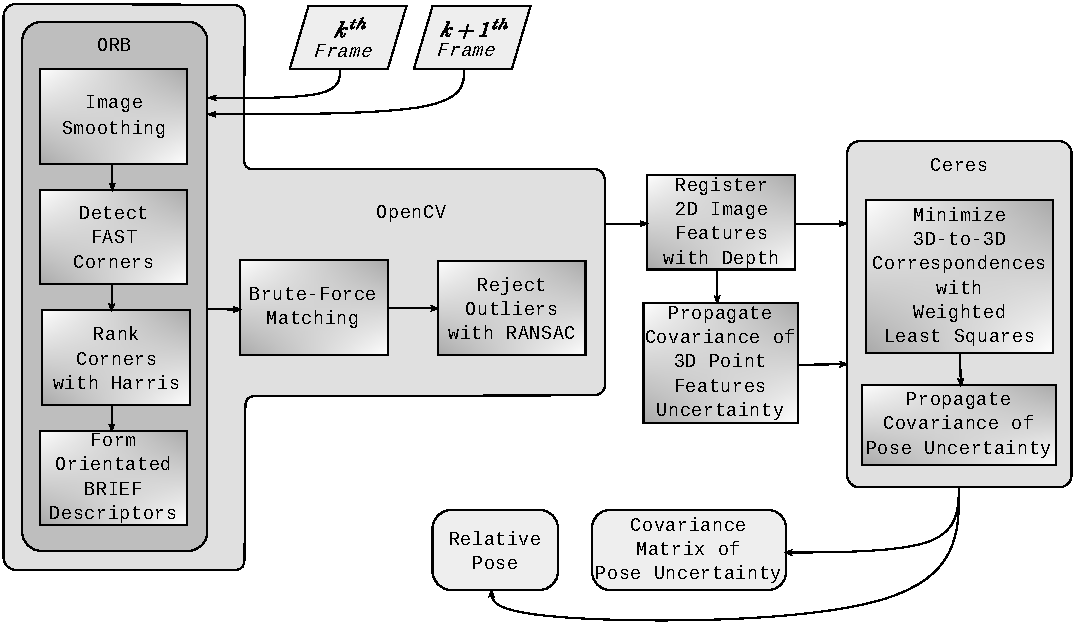
\includegraphics[width=0.9\linewidth,natwidth=640,natheight=640]
{fig/drawings/covo.pdf} \caption[CoVO Pipeline]{CoVO: The source code of the
implementation can be found in:
\href{https://github.com/ugurbolat/CoVO}{https://github.com/ugurbolat/CoVO}}
\label{fig:covo_pipeline} \end{figure}

Many VO systems require parameter tuning process and have algorithmic
variations.  Thus, building a reliable VO can be a daunting task.  To minimize
implementation errors and development time, we take advantage of two commonly
used open source libraries; i.e., OpenCV \parencite{opencv} for handling 
image
feature manipulations and Ceres \parencite{ceres-solver} for optimization. We
chose these two libraries because they are mature open source projects that
ensure efficiency and allow required customization.  In the following part of
this section, we will explain the essential steps that we take to build CoVO:


\begin{enumerate} 
  \item \textbf{Extracting Feature:} We choose ORB due to its efficiency and
    repeatability. Before extracting ORB features, we convert RGB images to
    grayscale. Then, we detect corners with FAST-9 that takes a patch of
    circular radius as 9 pixels around the corner. Next, the detected corners
    are ranked with Harris filter according to their image derivatives. In this
    way, we can query top N corners.  Finally, orientated BRIEF descriptors are
    formed by randomly selected pairs.  Note that these functionalities are
    already available in OpenCV and they are built based on 
    \parencite{Rublee2011a}.  
  \item \textbf{Matching Features:} After extracting ORB features from
    consecutive images, we matched them with Brute-Force algorithm that uses
    a Hamming window for the comparison. Before calling two features as a 
    match,
    the cross-check is performed to make sure both features are identified as a
    match in their own comparison set.  In the end, a filtering operation is
    applied on the matches by removing the worst 10\% matches based on the 
    distance
    calculated by the Hamming window.
  \item \textbf{Rejecting Outliers:} With the remaining matches, we apply
    RANSAC to reject outliers. Note that we choose RANSAC threshold to be 10
    pixels. Also, remember that we will have pseudo inliers even after applying
    RANSAC and the pixel errors are not particularly bounded with 10 pixels.
    The effect of pseudo inliers in pixel uncertainty is discussed in section
    \ref{sc_pseudo_inliers}.
  \item \textbf{Register 2D Features With Depth:} At this step, we simply
    combine inlier 2D features with their corresponding depth information. It
    is critical to note that Kinect has invalid depth measurement which is
    measured as 0 disparity level for certain regions of the object surface.
    Thus, we remove 2D features having invalid depth value from the match set.
    Plus, we remove 2D features that have a depth value greater than $5m$ since
    it is Kinect's accurate depth distance range. 
  \item \textbf{Preparing Covariance Matrix of 3D Feature Points:} For every
    inlier matched features, we propagate pixel uncertainties
    $\mathbf{Q_{uvz}}$ from image plane to camera coordinate system
    $\mathbf{Q_{xyz}}$ with the Jacobian of back-projection function
    $\mathbf{J_{bp}}(\mathbf{u})$ (see notation \eqref{eq:cov_xyz_prop}). This
    step is crucial for both improving for pose estimation results and
    estimating pose covariance.  
  \item \textbf{Minimizing 3D-to-3D Correspondences With Weights:} To able to
    take advantages of feature covariances of both consecutive images, we
    expand the residuals by defining both back-transformation and 
    forward-transformation
    function (see notation \eqref{eq:residuals_w_back_and_forward}).  It 
    improves
    the optimization process because we take measurement error in both images.
    The technique is taken from \parencite[see][101]{RichardHartley2003}.  
    Then, 
    the
    weighted least squares problem is solved by Levenberg-Marquardt by
    minimizing the error between 3D-to-3D correspondences to calculate relative
    camera pose.  
  \item \textbf{Calculating Covariance Matrix of the Estimated Pose:} After
    completing least squares optimization process, we calculate the covariance
    $\mathbf{Q_{tq}}$ of the estimated relative camera pose by propagating it
    from the feature covariances $\mathbf{Q_{xyz}}$ with the Jacobian of
    residuals function $\mathbf{J_{tqm}}(\mathbf{x^*})$ at the optimal 
    solution (see
    notation \eqref{eq:cov_tq_prop}).  Due to the non-linearity of the 
    projection
    function, an approximated version of the error propagation law produces
    overconfident covariance estimations. Thus, we scale the resulting
    $\mathbf{Q_{tq}}$ with $\phi$ to keep the estimator conservative.  The
    reason why we have this heuristic parameter is discussed in section
    \ref{sc_cov_eval}.  
\end{enumerate}

Note that all of the parameters mentioned above of CoVO are given in Table 
\ref{tb:covo_param}.  In the end, building such a VO system
require many tuning parameters and many VO algorithms do not emphasize the
effect of this phenomena.  The fact that we aim to develop an error-aware VO
that produces metric pose covariances means that each parameter must be
examined.  In the following sections of this chapter, we will discuss the
necessary components and parameters of the CoVO pipeline to highlight what is
required for an error-aware system.

\section{Modeling Uncertainty of RGB-D Camera} \label{sc_modeling_uncertainty_of_rgbd}

The main reason why conventional VO applications do not provide any uncertainty
information (namely covariance matrix) for its pose estimation is that it is
hard to model error characteristics of the whole VO pipeline.  This is because
we perform many preprocessing, each of which eventually introduces different
types of error. What we aim is to define the potential error source of the VO 
and
to model them. Thus, we will investigate the noise characteristic of sensors in
RGB-D camera in this section. In particular, we examine Kinect, having three
sensors: RGB camera, IR camera, and IR laser projector.  In our experiments and
evaluations, we assume that these sensors are calibrated such that there is no
registrations error when mapping RGB pixels to disparity pixels.

Furthermore, we assume that measurements with these sensors are independent of
each other.  Under this assumption, we split the source of errors into two
categories: feature related and depth-related uncertainties. The former is
caused by point feature location and matching algorithms. The latter is caused
by the depth camera sensor.  Let's see how we can model these two error sources
and how to form an uncertainty model for Kinect so that we estimate
metric covariance matrices for each relative camera pose.

\subsection{Feature Related Uncertainty} \label{sb_sc_pixel_uncertainty}

Our VO pipeline heavily relies on the detected features. For a VO algorithm to
operate reliably, it is expected that you will have a video stream that has
small translation and rotation differences at the consecutive images. Thus,
when pairing images to find common features, we expect not to have high-degree
rotation or a large amount of scaling on image features so that matching
algorithm would not suffer from a high number of outliers. Under these
circumstances, we identify two main error sources related to features; i.e.,
interest point location uncertainty and outliers in feature matching.


To understand these two types of errors, we need to remind ourselves how we
detect and describe features in the first
place (see Section \ref{sc_feature_extraction}).  In ORB, FAST corner filter 
is performed by selecting pixel coordinates
of an interest point and comparing it with its surrounding pixels. In an ideal
scenario where we match features in consecutive image perfectly, we would
assume that the error will be a half pixel due to the quantization process of
the RGB camera.  The ideal scenario breaks once we have outliers. 
In other words, if we had perfect matches, all the reprojected features would
be situated close to their matches and the error distance between matches
would be a half pixel. However, we still have outliers even after applying
RANSAC. Thus, the error distance for those outliers would be greater that one
pixel.  In this thesis, we call those outliers that appear after RANSAC
\textit{pseudo inliers}. Moreover, instead of taking pixel errors a half pixel,
we investigate the pixel error caused by pseudo inliers in section
\ref{sc_pseudo_inliers} and treat them as pixel uncertainty.

\begin{figure}[H] \centering
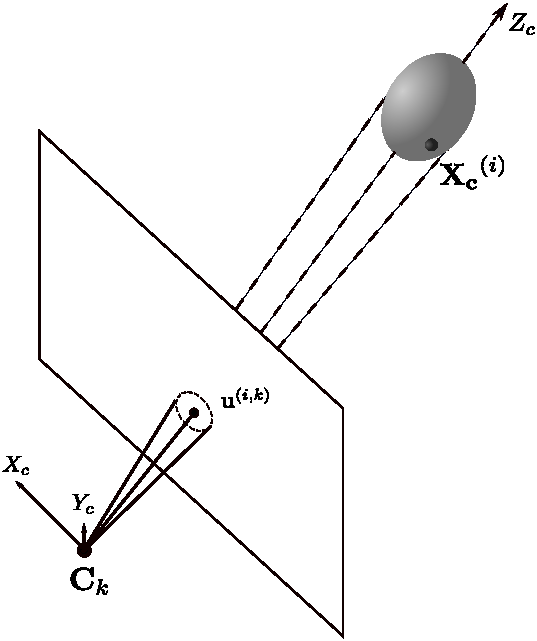
\includegraphics[width=0.6\linewidth,natwidth=640,natheight=640]
{fig/drawings/conic_ray.pdf} \caption[The Conic Ray Error Model]{ The conic ray
model is inspired from \parencite{Sola2007a} and we expand a confidence 
ellipse 
to a
confidence ellipsoid by adding depth uncertainty since we use an RGB-D camera.}
\label{fig:conic_ray_3d_error_model} \end{figure}

Having all these in mind, let's model uncertainty related to features.  First
of all, remember that 3D point features in the camera coordinate system are
projected to 2D points on an image plane with the pinhole model from section
\ref{sc_pinhole}.  When the aperture of a digital camera opens, it captures
incoming light rays using its light detector sensor and turns them into 
electrical signals, which is an over-simplified
definition of a camera. With the help of the pinhole model, one can build a
model for light ray coming from a 3D point.  Because we have the errors as
mentioned above, we can't measure the exact location of the 3D point feature.
However, it is likely that the point is within the dash line region (see figure
\ref{fig:conic_ray_3d_error_model}) As a consequence, we form an uncertainty
region which we call \textit{conic ray}.  Within this conic ray, we can
represent the uncertainty of a point with a \textit{confidence} ellipsoid if
the depth uncertainty is included.  To formulate this uncertainty, we need to
find parameters of the confidence ellipsoid which can be represented with
multi-dimensional Gaussian distributions in 3D space:

\begin{equation} \mathbf{g}_{xyz}(\mathbf{X}^{\mathcal{C}}) =
\frac{1}{\sqrt{(2\pi)^3|\mathbf{Q_{xyz}}|}} \exp(-\frac{1}{2}
(\mathbf{X}^{\mathcal{C}}-\mathbf{m_X}^{\mathcal{C}})^\top
\mathbf{Q_{xyz}}^{-1} (\mathbf{X}^{\mathcal{C}}-\mathbf{m_X}^{\mathcal{C}}))
\end{equation} \label{eq:cov_ellipse}

where $\mathbf{X}^{\mathcal{C}} = \begin{bmatrix} X \\ Y \\ Z\end{bmatrix}$ is
the real position of the point in the camera coordinate system,
$\mathbf{m_X}^{\mathcal{C}} = \begin{bmatrix} m_X \\ m_Y \\ m_Z \end{bmatrix}$
is the measured position, and $\mathbf{Q_{xyz}} = \begin{bmatrix} \sigma_X^2 &
\sigma_X\sigma_Y & \sigma_X\sigma_Z \\ \sigma_Y\sigma_X & \sigma_Y^2 &
\sigma_Y\sigma_Z\\ \sigma_Z\sigma_X & \sigma_Z\sigma_Y &
\sigma_Z^2\end{bmatrix}$ is the covariance of measurement error.  Notice that
errors in $x,y$ and $z$ direction are correlated to each other as the ellipsoid
can be tilted with respect to the focal point of the camera.  With regards to
measurement error in $x$ and $y$ direction, we only have indirect knowledge
since we measure features on image plane in $u$ and $v$ direction.  As to
measurment error in $z$ direction, we have direct knowledge (we assume that
disparity data is already converted to depth information).  As a matter of
fact, $(u,v,Z)$ form a special space $\R^3$ called \textit{disparity image
space}.  To get errors in $x$ and $y$ directions, we need to propagate pixel
uncertainties from image plane to camera coordinate system. Thus, we remind
ourselves with the back-projection function:

\begin{equation} \mathbf{X}^{\mathcal{C}} = \mathbf{F_{bp}}(\mathbf{u})
\end{equation}

\begin{equation} \begin{bmatrix} X \\ Y \\ Z \end{bmatrix} = \begin{bmatrix}
\frac{Z}{f_x} & 0 & -\frac{Z c_x}{f_x} \\ 0 & \frac{Z}{f_y} & -\frac{Z
c_y}{f_y} \\ 0 & 0 & Z \end{bmatrix} \begin{bmatrix} u \\ v \\ 1 \end{bmatrix}
\end{equation}

One can represent the probability distribution of the pixel and depth error
with another multivariate Gaussian distribution formed by pixel uncertainties. 

\begin{equation} \mathbf{g}_{uvz}(\mathbf{X}^{\mathcal{D}}) =
\frac{1}{\sqrt{(2\pi)^3|\mathbf{Q_{uvz}}|}} \exp(-\frac{1}{2}
(\mathbf{X}^{\mathcal{D}}-\mathbf{m_u}^{\mathcal{D}})^\top
\mathbf{Q_{uvz}}^{-1} (\mathbf{X}^{\mathcal{D}}-\mathbf{m_u}^{\mathcal{D}}))
\end{equation} \label{eq:cov_ellipse}

where $\mathbf{X}^{\mathcal{D}} = \begin{bmatrix} u \\ v \\ Z\end{bmatrix}$ is
the real pixel coordinates and the corresponding depth value in disparity image
space, $\mathbf{m_u}^{\mathcal{D}} = \begin{bmatrix} m_u \\ m_v \\ m_Z
\end{bmatrix}$ is the noisy pixel measurements along with the noisy depth
measurement, and $\mathbf{Q_{uvz}} = \begin{bmatrix} \sigma_u^2 & 0 & 0\\ 0 &
\sigma_v^2 & 0 \\ 0 & 0 & \sigma_Z^2\end{bmatrix}$ is the covariance of these
measument errors as pixel and depth measurements are considered independent.

To convert disparity image space to camera coordinate system, we utilize the
error propagation low. In this respect, we need the partial derivative of the
back-projection function:

\begin{equation} \label{eq:jacob_back_proj}
  \mathbf{J_{bp}}(\mathbf{u}) = \frac{\partial
\mathbf{F_{bp}}(\mathbf{u})}{\partial \mathbf{u}}  = \begin{bmatrix}
\frac{Z}{f_x} & 0 & (\frac{u}{f_x} - \frac{c_x}{f_x}) \\ 0 & \frac{Z}{f_y} &
(\frac{v}{f_y} - \frac{c_y}{f_y}) \\ 0 & 0 & 1 \end{bmatrix} \end{equation}

Then, we propagate the pixel covariances as follows:

\begin{equation} \mathbf{Q_{xyz}} = \mathbf{J_{bp}}(\mathbf{u})^\top
\mathbf{Q_{uvz}} \mathbf{J_{bp}}(\mathbf{u}) \end{equation}


Apart from pixel uncertainties, what we haven't discussed is how we get the
$\sigma_Z$ depth uncertainty.  It deserves own explanation so we will cover in
the next section.

\subsection{Depth Related Uncertainty} \label{sb_sc_depth_uncertainty}

Modeling noise in depth measurements is more complicated than an RGB camera.
In Section \ref{sc_depth_model}, remember that we explained how structured IR
light speckles are projected onto an object so that IR camera can capture its
deformed patterns.  During this process, many things can go wrong. For example,
(1) specific ambient background would make Kinect suffer from over-saturated
disparity image, (2) having multiple Kinect in the same environment can lead to
interference issue, (3) multi-path propagation of the light might change the
expected illumination, or (4) measuring in dynamic scene might result in
improper IR light patterns. All of these non-deterministic events makes it
harder to model uncertainty. However, we assume that operating conditions
and environment are chosen carefully to avoid these events as much as possible.
What we aim to model in this section is mostly systematic errors in Kinect. In
this regard, we rely on the experiments conducted by \parencite{Nguyen2012a}. 

\subsubsection{Kinect's Systematic Depth Noise}

The experimental analysis contributed to model Kinect's depth noise.
\parencite{Nguyen2012a} calculated the difference between ground truth and 
Kinect
measurements and,  found out that there are two types of systematic noise
occurring in Kinect's depth measurements: \textit{axial} noise and
\textit{lateral} noise.  Note that our depth noise model is based on their
work.


\begin{figure}[H] \centering
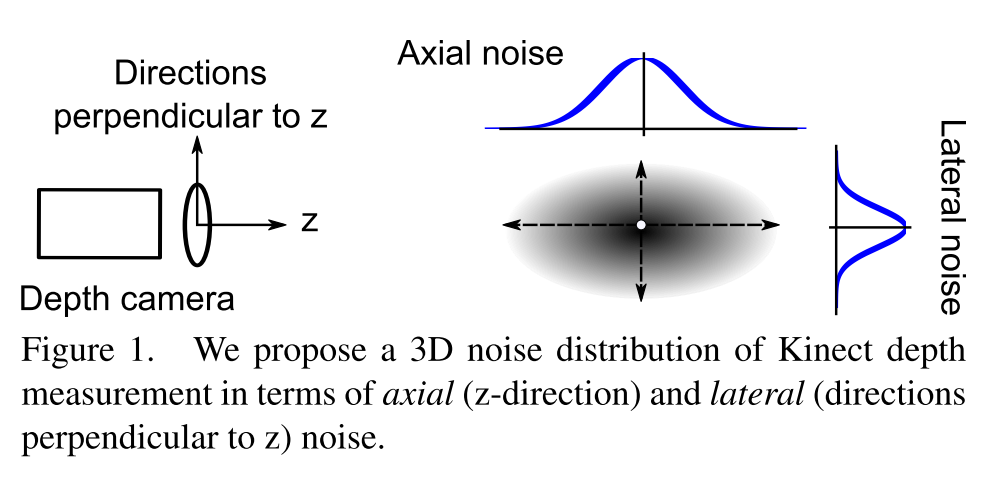
\includegraphics[width=0.7\linewidth,natwidth=640,natheight=640]
{fig/ref_imgs/kinect_noise_model.png} \caption[Kinect's Depth Noise
Model]{According to \parencite{Nguyen2012a}, axial noise corresponds to noise 
along
the z-axis in the camera coordinate system. In other words, it is the depth
uncertainty model we search for our conic ray model.  On the other hand,
lateral noise corresponds to directions perpendicular to the $z$ axis. This
noise creates uncertainty in the pixel coordinates of the disparity image.
The figure is taken from \parencite{Nguyen2012a}.} 
\label{fig:kinect_noise_model}
\end{figure}

To detect the lateral and axial noise, they built an experimental setup with a
Kinect that projects its IR speckle patterns onto a planar surface.  Then, they
collected depth measurements at a different distance to the planar surface
positioning at different angles.  For calculating the axial noise, they first
removed the lateral noise cropping edges. Then, the remaining depth region was
fitted to a plane that has the minimum error to the ground truth. Finally, they
calculated the distance difference between measured depth and ground truth.
Whereas, the lateral noise was simply calculated by taking pixel difference
between fitted straight edge passing through the center of distribution and
measured (zigzag-like shape) pixels. The illustration of this experiment is
given in Figure \ref{fig:kinect_noise_experiment}.

\begin{figure}[H] \centering
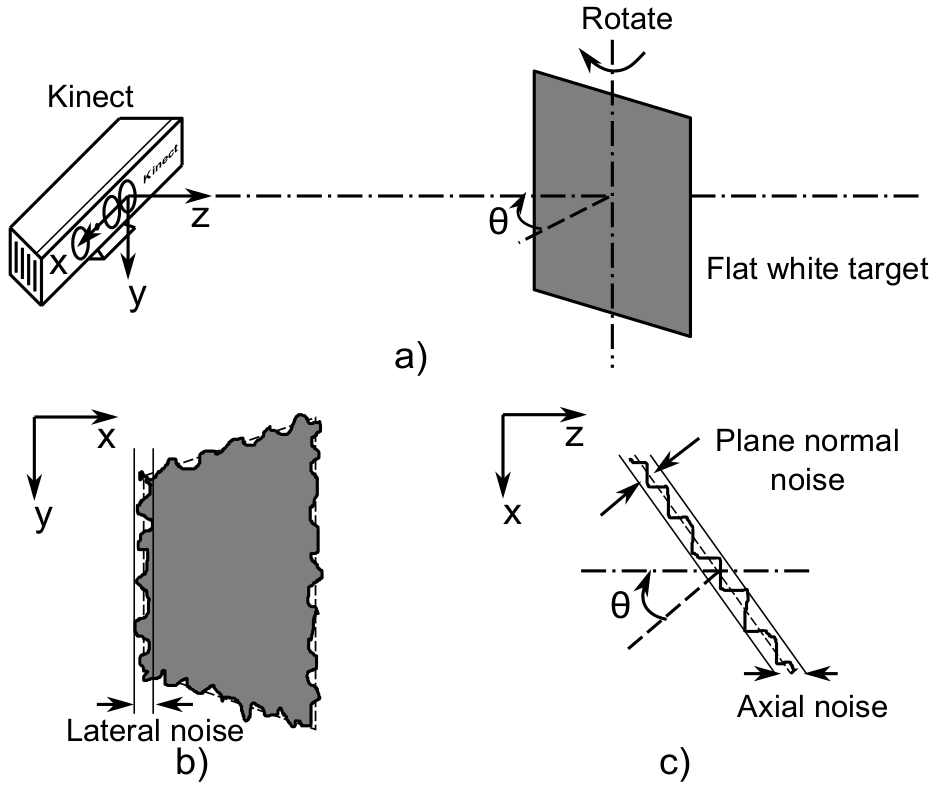
\includegraphics[width=0.7\linewidth,natwidth=640,natheight=640]
{fig/ref_imgs/kinect_noise_experiment.png} \caption[Kinect's Depth Noise
Experiment]{In order to measure the depth noise, an object that has a flat 
white
surface was placed at different known distances to Kinect. During the
experiments, they also discovered that depth noise changes when the angle of
the object changes with respect to Kinect's focus point. Thus, they included
different poses with different angles by rotating the object (a).  The effect
of lateral and axial noise is depicted in (b) and (c).  The figure is taken
from \parencite{Nguyen2012a}.} \label{fig:kinect_noise_experiment} \end{figure}

After calculating errors between measurements and ground truth, they realized
that the axial and lateral noise have different noise characteristics. The
lateral noise error distribution stays constant with the distance, while the
axial noise distribution gets wider with the increased range.

Besides, the axial noise has another property, which is the response to the
different angles. It was observed that the standard deviation of the axial
noise increases drastically after 60 degrees.  In the light of these
experiments, they proposed two empirical models that fit corresponding
measurements for the axial and lateral noise.  For axial noise, they define a
quadratic relationship between the standard deviation of the error and distance
along the z-axis. 

\begin{equation}\label{eq:depth_noise_model} \sigma_Z (Z,\theta) = 0.0012 +
0.0019 \cdot (Z-0.4)^2 \text{, if } \ang{10}\leq \theta \leq \ang{60}
\end{equation}

where $Z$ is the measured depth in meters.  Plus, they added a hyperbolic
parameter to represent the behavior measurement error beyond 60 degrees:

\begin{equation} \sigma_Z (Z,\theta) = 0.0012 + 0.0019 \cdot (Z-0.4)^2 +
\frac{0.0001}{\sqrt{Z}} + \frac{\theta^2}{(\pi/2 - \theta)^2} \text{, if }
\theta \geq \ang{60} \end{equation} \label{eq:axial_noise_w_hyperbolic}

For lateral noise, its noise was almost constant with respect to distance along
the z-axis and had a similar hyperbolic effect after 60 degrees of angle.
Hence, they defined lateral noise with the following equations:

\begin{equation} \sigma_L(\theta) = 0.8 + 0.035 \cdot \theta/(\pi/2-\theta)
\text{ (in pixels)} \end{equation}

To validate these experimental noise models' correctness, they implemented a 3D
reconstruction and a camera pose tracking scenario.  As a consequence, they
observed that the noise models improved the overall accuracy of both
applications. It is important to note that they cooperated the iterative
closest point (ICP) to estimate the camera poses. The ICP is one of many
algorithms to solve VO problem.  With the ICP, one utilizes all or most of the
3D point clouds instead of selecting a distinct feature in each frame. Now that
we know how depth noise is modeled, we can plug it into our noise model:

\begin{equation} \mathbf{Q_{uvz}} = \begin{bmatrix} \sigma_u^2 & 0 & 0 \\ 0 &
\sigma_v^2 & 0 \\ 0 & 0 & (\sigma_Z^{(i)}(Z, \theta))^2 \end{bmatrix}
\end{equation}

While the axial noise can be embedded as the third dimension along the z-axis,
the lateral noise has an indirect relationship to the overall uncertainty of a
point feature. This indirect relationship occurs when associating depth pixel
coordinates with the pixel coordinates, namely \textit{registration}.
Therefore, one can avoid this registration error by applying a smoothing filter
on depth images.  According to their experiments, the lateral noise of the
Kinect is around one pixel.  Thus, a 3x3 smoothing filter can be used on
extracted features or edges in the disparity image.

In short, the probabilistic model, we built with the conic ray, and the
confidence ellipsoids, based on normal distribution can now allow us to
estimate relative camera poses with the weighted least squares optimization.
To construct a cost function for the least squares problem, we need to gather
(1) measured pixels, (2) measured depth, (3) calibrated intrinsic camera
parameter and most importantly (4) covariance matrices of the measurements.
Having covariance matrices for the point feature measurements not only improves
the convergences of the optimization algorithm but also enables us to estimate
a covariance matrix for the estimated relative pose. 



\section{Pose Estimation with Uncertainties} \label{sc_rel_pose_est_w_uncertainty}

Before diving into the formulation, it is a good idea to refresh our knowledge
about how we estimated the relative pose of a camera using 3D-to-3D 
correspondences
in Section \ref{sb_sc_3d_to_3d}.  Remember that after pre-processing extracted
features, we would have $m$ number of measured feature matches in camera
coordinate system with respect to $k^{th}$ and $k+1^{th}$ consecutive camera
frames and we stored them as $(\mathbf{X}^{(k,1:m)},
\mathbf{X}^{(k+1,1:m)})$. 
%Note that we drop $\mathcal{C}$
%superscript for simplicity and assume that all point features are in the 
%camera
%coordinate system.  
The transformation relationship between the $k^{th}$ frame
and the $k+1^{th}$ frame was defined with the translation $\mathbf{t}_{k,k+1}$
and rotation $\mathbf{q}_{k,k+1}$ information, which we want to know.  As
discussed earlier, the main idea was to back-transform the
$\mathbf{X}^{(k+1,1:m)}$ features onto $\mathbf{X}^{(k,1:m)}$ features so
that they are aligned with respect to the same camera frame.  Then, we minimize
the error while optimizing the translation and rotation.  Here, we define the
back-transform function as follows:

\begin{equation} f_b(\mathbf{x}_{k,k+1}, \mathbf{X}^{(k+1,i)}) =
\mathbf{q}_{k,k+1} \otimes \mathbf{X}^{(k+1,i)} \otimes \mathbf{q}_{k,k+1}^*
+ \mathbf{t}_{k,k+1} \end{equation}

In the traditional VO problem, the residuals function of the optimization
problem is defined by the difference only between back-transformed point
features from $k+1^{th}$ and measured point features from $k^{th}$.

\begin{equation} \mathbf{t}_{k,k+1}^*, \mathbf{q}_{k,k+1}^* =
\argmin_{\mathbf{t}_{k,k+1}, \mathbf{q}_{k,k+1}} \sum_i|| \mathbf{X}^{(k,i)} -
f_b(\mathbf{t}_{k,k+1}, \mathbf{q}_{k,k+1}, \mathbf{X}^{(k+1,i)})||^2
\end{equation}

The important part of the error-aware VO that we propose in this thesis lies on
having estimated uncertainty of the features and then to propogate it through
uncertainty of estimated relative pose.  If we utilized our conic ray model, we
would have different covariance matrices for each feature.  Thus, let's include
covariance matrices into the optimization problem:

\begin{equation} \underbrace{\mathbf{t}_{k,k+1}^*,
\mathbf{q}_{k,k+1}^*}_{\mathbf{x^*_{k,k+1}}} =
\argmin_{\underbrace{\mathbf{t}_{k,k+1},
\mathbf{q}_{k,k+1}}_{\mathbf{x}_{k,k+1}}} \sum_i||
\underbrace{\mathbf{X}^{(k,i)} - f_b(\mathbf{t}_{k,k+1}, \mathbf{q}_{k,k+1},
\mathbf{X}^{(k+1,i)})} _{\mathbf{r}^{(i)}_{b}(\mathbf{x}_{k,k+1})}
||^2_{\mathbf{Q}^{(k+1,i)}_{\mathbf{xyz}}} \end{equation}


However, this residuals function builds on the assumption that features from
the $k^{th}$ frame are noise-free and features from the $k+1^{th}$ frame are
noisy.  Thus, we could only weight with $\mathbf{Q}^{(k+1,1:m)}_{\mathbf{xyz}}$
as seen in the above equation.  In reality, we know that the features from both
frames are noisy. We can consider including forward-transform function such
that we also take all covariance matrices
$(\mathbf{Q}^{(k,1:m)}_{\mathbf{xyz}}, \mathbf{Q}^{(k+1,1:m)}_{\mathbf{xyz}})$
for all features into account during optimization.  In this case, one needs to
calculate both back-transform and forward-transform for the residuals function.

\begin{figure}[H] \centering
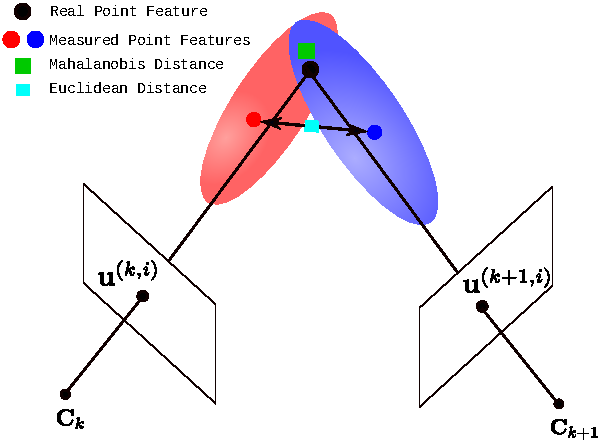
\includegraphics[width=0.9\linewidth,natwidth=640,natheight=640]
{fig/drawings/feature_uncertainty.pdf} \caption[Pose Estimation With Feature
Uncertainty] {When matched image features are back-projected onto the camera
coordinate system, they are supposed to overlap. In practice, they are located
at different positions due to the noise. This effect is illustrated with red
and blue points, both of which refers to the black point that is the real
position of the measured point feature. In the absence of an uncertainty model
of these point features, one can only minimize the Euclidean error distance,
which degrades pose estimation accuracy. Conversely, one can model the point
feature uncertainty with the conic ray model and minimize the Mahalanobis
distance. This is the method we utilize in our VO.} \label{fig:min_mahalanobis}
\end{figure}

With being said, we can now extend the residuals function of our optimization
problem by adding forward-transform.  Let's define the auxiliary function in 
the
following form:

\begin{equation} \mathbf{r_{f}}^{(i)}(\mathbf{x}_{k,k+1}) =
\mathbf{X}^{(k+1,i)} - f_f(\mathbf{x}_{k,k+1}, \mathbf{X}^{(k,i)})
\end{equation}

where the forward-transform function is defined as:

\begin{equation} f_f(\mathbf{x}_{k,k+1}, \mathbf{X}^{(k,i)}) =
\mathbf{q}_{k,k+1}^* \otimes (\mathbf{X}^{(k,i)} - \mathbf{t}_{k,k+1})
\otimes \mathbf{q}_{k,k+1} \end{equation}

Now we can reformulate our optimization problem by adding forward and
back-transformation to each other along with corresponding covariance matrices:

\begin{equation} \label{eq:residuals_w_back_and_forward} \mathbf{x^*}_{k,k+1} =
\argmin_{\mathbf{x}_{k,k+1}} \sum_i
||\mathbf{r_b}^{(i)}(\mathbf{x}_{k,k+1})||^2_{\mathbf{Q}^{(k+1,i)}_{\mathbf{xyz}}}+
||\mathbf{r_f}^{(i)}(\mathbf{x}_{k,k+1})
||^2_{\mathbf{Q}^{(k,i)}_{\mathbf{xyz}}} \end{equation}

With the new auxiliary function, we can minimize the error on both forward- and
back-transformation.  In this way, we include noise occurring in both images
into the optimization process. This technique is taken from
\parencite[see][101]{RichardHartley2003} and is called \textit{error in both 
images}.
Furthermore, we expand the technique, whose original version is to minimize the
Euclidean error distance, to minimize \textit{Mahalanobis} error distance by
including feature covariances (see Figure \ref{fig:min_mahalanobis}).

Let's reformulate the residuals functions in the form of a matrix to simplify
the notation for the optimization problem.  Hence, a single back-transformation
operation for a single feature match is a $\mathbf{r_b}^{(i)}$ single residual
block function.  The same definition applies for the forward-transformation
with $\mathbf{r_f}^{(i)}$.  Note that we only use $\frac{1}{2}$ in front of the
residuals function for cosmetics reasons as it does not effect convergence of
the optimization process.  Here, we reorginize the residual blocks by stacking
residual blocks by columns:

\begin{equation} \label{eq:residuals_w_back_and_forward_matrix}
  \begin{aligned} \mathbf{x}^*_{k,k+1} :=
\argmin_{\mathbf{x}_{k,k+1}} \frac{1}{2} \begin{Vmatrix}
\mathbf{r_b}^{(1)}(\mathbf{x}_{k,k+1}) \\
\mathbf{r_f}^{(1)}(\mathbf{x}_{k,k+1}) \\ \vdots \\
\mathbf{r_b}^{(m)}(\mathbf{x}_{k,k+1}) \\
\mathbf{r_f}^{(m)}(\mathbf{x}_{k,k+1})
\end{Vmatrix}^2_{\mathbf{Q}^{k,k+1}_{\mathbf{xyz}}}
\end{aligned} \end{equation}

Above equation is the final residuals function that we are going to minimize.
LM algorithm can be used for the optimization. I refer readers for the
fundamental theory behind the algorithm to Appendices
\ref{sc_least_squares}.  However, we also need to extend regular least squares
problem to weighted least squares problem since we multiply residual blocks
with inverse covariance matrices.  Let's omit $(k,k+1)$ part and generalize the
problem for convenience:

\begin{equation} \begin{aligned} \mathbf{x}^* = \argmin_{\mathbf{x}}
F(\mathbf{x}) & = \argmin_{\mathbf{x}} \frac{1}{2}
||\mathbf{r}(\mathbf{x})||^2_{\mathbf{Q_{xyz}}} \\ & = \frac{1}{2}
\mathbf{r}(\mathbf{x})^\top \mathbf{Q_{xyz}}^{-1} \mathbf{r}(\mathbf{x}) 
\\ & =
\frac{1}{2} \mathbf{r}(\mathbf{x})^\top \mathbf{\Omega}_{\mathbf{xyz}}
\mathbf{r}(\mathbf{x}) \end{aligned}
\end{equation}\label{eq:residuals_objective}

where $\mathbf{\Omega_{xyz} = Q^{-1}_{xyz}}$ is the \textit{information
matrix}, represent a relationship between covariance matrices and weighting
process.  That is, the smaller covariance (smaller the uncertainty in other
words) for features, the greater weight will have in the optimization.  In this
respect, LM will attempt to converge to an optimal solution in which the
rotation and translation information is sufficient by iteratively updating the
state vector:

\begin{equation} \mathbf{x}^{n+1} = \mathbf{x}^{n} \boxplus \Delta \mathbf{x}
\end{equation}

where $\boxplus$ refers to a manifold operation.  The translational part of the
state vector is in Euclidean space. Thus, one can update the state vector with
a regular vector addition operation.  However, this addition operation does not
produce good results for the rotational part. This is because the rotation is
the tangent space.  For the further details of the optimization on a manifold
for our VO, I refer readers to Appendices \ref{sc_lsq_manifold}.

To sum up, we explained how we form the residuals function for the optimization
by including back-transform and forward-transform function. We also extended
the regular least squares to weighted least squares problem by incorporating
the feature covariances. In the following section, we will describe how to
propagate the pose covariances.


\section{Covariance of the Estimated Pose} \label{sc_covariance_estim} 

Another important question one can ask in any odometry applications is that
what is the uncertainty, namely covariance, of the odometry measurements?
Generally, traditional VO algorithms do not provide an answer to this question
since it does not take the uncertainty of the features into account.  This
issue introduces a big drawback, especially in sensor applications.  However,
we are now able to estimate a covariance matrix of the estimated pose since we
use the conic ray to model feature uncertainties.  With the help of each pose
covariance, we can represent the possible accumulated covariances along the
trajectory with $3\sigma$ ellipsoids if the relative poses are concatenated as
seen in Figure \ref{fig:pose_uncertainty}. 

The fact that we use a metric uncertainty model to represent 3D point features'
noise enables us to estimate a metric pose uncertainty. This property will
produce more accurate pose covariance matrices.  For example, if we had only
detected 3D point feature matches positioned far from Kinect, the pose
covariance would get larger compared to the situation where the features are
placed close to Kinect.  Another determinant is the number of detected feature
matches. Having an insufficient number of features would increase the
covariance as well.  All of these will contribute to the robustness of sensor
fusion applications.  Now that we discuss the importance of having such a
dynamic uncertainty estimation, we will provide the formulation for estimating
the pose covariance matrix in the following part. 

\begin{figure}[H] \centering
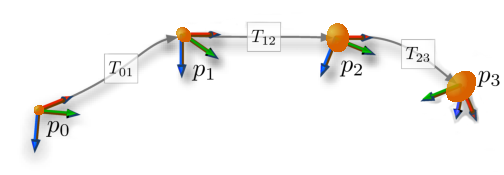
\includegraphics[width=0.7\linewidth,natwidth=640,natheight=640]
{fig/drawings/pose_uncertainty.pdf} \caption[Pose Uncertainty]{This is an
illustration to ellipsoids for pose uncertainties that are growing with every
relative pose estimations. In the absence of absolute sensors that measure the
priori-known landmarks, the pose drift will grow forever.}
\label{fig:pose_uncertainty} \end{figure}

Calculating a covariance matrix for the estimated state vector parameters is
fairly straightforward if the optimization for the relative camera pose is
performed as described in the previous section. We can simply utilize the
\textit{error propagation law}, which I refer readers to Appendices
\ref{sc_error_prop_law} for further details of the theory.  In this case, we
require the Jacobian matrix at the optimal solution and corresponding
covariance  matrices for each point feature. Then, we can propagate them to get
the covariance for the estimated parameters by applying the following equation:

\begin{equation}\label{eq:cov_tq_prop} \mathbf{Q}_{\mathbf{tq}}^{k,k+1} =
(\frac{1}{2})^2 \cdot \mathbf{J_{tqm}}(\mathbf{x^*}_{k,k+1})^\top
\mathbf{Q}_{\mathbf{xyz}}^{k,k+1} \mathbf{J_{tqm}}(\mathbf{x^*}_{k,k+1})
\end{equation}

where $\mathbf{J_{tqm}}(\mathbf{x^*}_{k,k+1}) \in \R^{6mx6}$ is the Jacobian of
extended residuals function with back-transformation, forward-transformation 
and manifold
in \eqref{eq:new_jacobian_chain_rule},

\begin{equation} \begin{aligned} & \mathbf{Q}_{\mathbf{xyz}}^{k,k+1}  =
\begin{bmatrix} \mathbf{Q}_{\mathbf{xyz}}^{(k,1)} & \dots & & &\mathbf{0} \\
\mathbf{0} & \mathbf{Q}_{\mathbf{xyz}}^{(k+1,1)} & &\dots & \vdots  \\ \vdots &
& \vdots &  &\\ &  & & \mathbf{Q}_{\mathbf{xyz}}^{(k,m)} & \mathbf{0} \\
\mathbf{0} &  & & & \mathbf{Q}_{\mathbf{xyz}}^{(k+1,m)} \end{bmatrix} \in
\R^{6mx6m} \end{aligned} \end{equation}

is the covariance matrix that comprised of all covarince matrices for all
matched features from $k^{th}$ and $k+1^{th}$ consecutive frames,

\begin{equation}\label{eq:cov_xyz_prop} \begin{aligned} &
\mathbf{Q}_{\mathbf{xyz}}^{(k,i)} = 
\mathbf{J_{bp}}^\top(\mathbf{u}^{(k,i)})
\begin{bmatrix} \sigma_u & 0 & 0 \\ 0 & \sigma_v & 0 \\ 0 & 0 &
(\sigma_Z^{(i)}(Z, \theta))^2 \end{bmatrix} \mathbf{J_{bp}}(\mathbf{u}^{(k,i)})
\in \R^{3x3} \end{aligned} \end{equation}

is the covariance matrix for the $i^{th}$ matched feature from $k^{th}$ frame 
where $\mathbf{J_{bp}}^\top(\mathbf{u}^{(k,i)})$ is the Jacobian matrix 
of 
back-project function (see notation \eqref{eq:jacob_back_proj}).

\begin{equation} \begin{aligned} & \mathbf{Q}_{\mathbf{tq}}^{k,k+1}  =
\begin{bmatrix} \sigma_{t_x}^2 & 0 & 0 & 0 & 0 & 0 \\ 0 & \sigma_{t_y}^2 & 0 &
0 & 0 & 0 \\ 0 & 0 & \sigma_{t_z}^2 & 0 & 0 & 0 \\ 0 & 0 & 0 & \sigma_{q_x}^2 &
0 & 0 \\ 0 & 0 & 0 & 0 & \sigma_{q_y}^2 & 0 \\ 0 & 0 & 0 & 0 & 0 &
\sigma_{q_z}^2 \end{bmatrix} \in \R^{6x6} \end{aligned} \end{equation}

is the resulting covariance matrix for the estimated state vector parameters.
In other words, we are now able to calculate the uncertainty of the estimated
pose of the camera.

Notice $(\frac{1}{2})^2$ in front of \eqref{eq:cov_tq_prop}.  In the original
error propagation law, this does not exist.  It comes from the fact that we use
both the back-transformation and forward-transformation in residuals 
function.  To be
more clear, remember that we represented a relative camera motion with both
back-transformation and forward-transformation to take errors on both $k^{th}$ 
and $k+1^{th}$
consecutive images into account. This resulted in having two residuals
$\mathbf{r_b}^{(i)}$ and $\mathbf{r_f}^{(i)}$ for one feature match (see
notation \eqref{eq:residuals_w_back_and_forward}).  Therefore, we divide by 2 
to
average. The reason we square it is because of the covariance.

Finally, let's summarize this chapter. At first, we provided a literature
background for an error-aware VO. Then, we argued that all the related work being
done did not use feature uncertainty to produce metric pose covariance. With
this motivation, we gave a recipe for building an error-aware VO which we call
CoVO. Afterward, we explained how we include feature and depth-related noise 
models
into the optimization process so that we propagate a covariance matrix for the
estimated relative camera pose. 
The main takeaway from this chapter is that in order to estimate 
pose covariances, we must have accurate models for both sensor and 
algorithmic errors. 
That being said, we will evaluate the
proposed CoVO algorithm with simulated and real-world data in the next chapter. 

\chapter{Evaluation} \label{cp_evaluation}
% ***************************CP5-EVALUATION***************************

Computer vision applications such as VO require many approximations and 
linearization techniques to cope with its dynamic nature for the sake of 
efficiency.  In practice, many corner cases might occur, no matter how good 
such estimation algorithms are modeled. It is therefore critical to verify 
such systems, especially in the real-world environment.  Considering that the 
proposed error-aware VO algorithm outputs two information: relative pose 
estimation and its covariance estimation, this chapter will mainly build 
around two following questions that I am going to ask:

\begin{enumerate} \item What is the \textit{accuracy} of relative pose 
estimations?  \item How \textit{consistently} do the algorithm estimate 
covariance of its pose?  \end{enumerate}

In order to tackle these questions, simulation environment will be used to validate the model at first. Then, TUM RGB-D datasets will be used to test the algorithm in real-world scenarios.

\section{Error Metrics}

There are already well-established error evaluation methods in literature so I am going to follow them to better understand the characteristics of the proposed algorithm.  If we want to apply these methods on our algorithm, we need to have the ground truth pose sequences $\mathbf{x}_{1:n} \in SE(3)$ for comparing with the estimated pose sequences $\mathbf{x^*}_{1:n} \in SE(3)$.  In our calculations, we assume that both pose sequences are time-synchronized, equally sampled and have the same length $n$.  However, it is important to note that none of these assumptions is held so in reality and we need to be aware of the error caused by these issues.  We attempt to minimize these issues by linearly interpolating the ground truth.


\subsubsection{Relative Pose Error}

For evaluating the accuracy of a VO algorithm, it is better to calculate the 
relative pose error rather than comparing with the absolute (whole) estimated 
trajectory. This is also referred to Relative Pose Error (RPE).  On the other 
hand, some VOs estimate a relative pose with frame-to-frame and some with 
keyframes.  To able to compare all kinds of VO with each other, a fixed time 
interval $\Delta$ is chosen for measuring the local accuracy of the pose 
estimation.  In this way, we take small local drifts into account to compare 
both types of VO algorithms.  Let's define RPE at time instance $i$ as follows:

\begin{equation}
  \mathbf{E}_i := 
  (\mathbf{x}_i^{-1} \mathbf{x}_{i+\Delta})^{-1} 
  (\mathbf{x^*}_i^{-1}\mathbf{x^*}_{i+\Delta})
\end{equation}

One can take a mean of all $E_{1:n}$, but this hides the effect of outliers 
when $n$ is large.  Instead, \parencite{Sturm2012a} suggests to calculate Root 
Mean Error 
Squared (RMSE) which encodes the error with much more information since it 
takes mean deviation of the error into account.
In other words, RMSE will show how the mean deviation of the error.  To calculate RMSE, $m = n - \Delta$ number of RPE are required among $n$ pose sequences:

\begin{equation}
  RMSE(\mathbf{E}_{1:n},\Delta) := \sqrt{\frac{1}{m} \sum_{i=1}^{m}||\mathbf{E}_i||^2}
\end{equation}

Then, we take a mean of all RMSE over whole trajectory:

\begin{equation}
  RMSE(\mathbf{E}_{1:n}) :=  \frac{1}{n} \sum_{\Delta=1}^{n}RMSE(\mathbf{E}_{1:n},\Delta)
\end{equation}

It is important to note that we take $\Delta=1$ when we want to know 
a drift per frame. This is useful when comparing simulation results with 
real-world experiment results for the same algorithm such as CoVO itself. 
Conversely, we take $\Delta=30$ when comparing 
the proposed algorithm other VO such as FOVIS. This case corresponds to a drift per approximately 
1 second.

\subsubsection{Normalized Estimation Error Squared}

The main focus of this thesis is to provide metric uncertainty of the relative pose estimations. We can estimate dynamic covariances thanks to propagation property of the feature covariances based on the conic ray error model. In this respect, it is critical to assess the consistency of estimated covariance values to use them safely in sensor fusion applications.  One of the good metrics to evaluate consistency is to calculate Normalized Estimation Error Squared (NEES). This method measures the credibility of the provided covariance, and it helps us to decide whether the predicted uncertainty values are optimistic or pessimistic.  One can calculate NEES if $\mathbf{x}_i$ real pose, $\hat{\mathbf{x}_i}$ predicted pose and $\Omega_i = \mathbf{Q}_i^{-1}$ information matrix are known at time instance $i$:

\begin{equation}
  \epsilon_i = (\mathbf{x}_i - \mathbf{x^*}_i)^\top \mathbf{\Omega}_i 
  (\mathbf{x}_i - \mathbf{x^*}_i) 
  = ||\mathbf{e}_i||^2_{\Omega_i}
\end{equation}

%\subsubsection{Average Normalized Estimation Error Squared (ANEES)}

For comparison reasons, we also take an average of NEES (ANEES) over whole trajectory:

\begin{equation}
  d \hat{\epsilon} =  \frac{1}{n} \sum_{i=1}^{n} \epsilon_i = 
  \frac{1}{n} \sum_{i=1}^{n} ||\mathbf{e}_i||^2_{\Omega_i}
\end{equation}

If the system is linear, has a degree of freedom $d=1$ and Gaussian noise, 
then the expected value 
$\hat{\epsilon}$ is 1. 

However, in practice, this does not hold. Therefore, besides ANEES, another 
metric when deciding on whether the estimator is consistent or not is to look 
at the distribution of NEES over trajectory.  It is expected that it is 
distributed as a chi-square $\chi_d^2$ with $d$ degrees of freedom.  For an 
estimator with 3 degrees of freedom, the acceptance region is $\hat{\epsilon} 
\in 
[2.5,3.5]$ when significance level $\alpha$ of $\chi_d^2$ is chosen 2.5\% and 
50 Monte Carlo runs according to \parencite[see][234--235]{Shalom2001}.  Thus, 
when evaluating the consistency of the estimator in simulation, we aim to get 
$\hat{\epsilon_t}=[2.5,3.5]$ for the translation and 
$\hat{\epsilon_q}=[2.5,3.5]$ for the rotation since both have 3 degrees of 
freedom. On the other hand, when testing the estimator with real-world data, 
we only take upper boundary of acceptance region $\hat{\epsilon_t} \in [0, 
3.5]$ and $\hat{\epsilon_q} \in [0, 3.5]$ since it is acceptable to have a 
conservative estimator rather than overconfident one.

\section{Simulation Environment}\label{sc_sim_env}

Before testing the proposed algorithm, we will validate the relative 
pose estimation and its covariance with the simulated data. Hence, 
we create a 3D simulation environment that consists of a camera pose, 
3D point features and their confidence ellipsoids. Our test scenario 
will be comprised of the following steps:

\begin{itemize}
  \item 500 3D point features $\mathbf{X}^{(\mathcal{C}, 1:500)}$ are created 
  within the camera's observable space.
  \item By utilizing the pinhole model (see notation 
  \eqref{eq:simplyfied_proj_func}), 
    all 3D point features are projected 
    onto the camera frame whose initial pose $\mathbf{x}_0^{\mathcal{C}}$ is known. 
    The intrinsic matrix $\mathbf{K}$ is taken similar to TUM RGB-D FR1  
    dataset (see Table \ref{tb:tum_calib_param}).
  \item Projected image features are stored in the form of 
    $(u^{(0, 1:500)}, v^{(0, 1:500)},z^{(0, 1:500)})$ sensor 
    measurements as you would usually get it from 
      a regular RGB-D camera. 
    \item The camera is transformed (rotated and translated) with a known transformation information 
      $\mathbf{T}_{0,1} = \mathbf{x}_{0,1} = [0.6, 0.6, 0.05, -0.183, -0.183, 0, 0.966]$ 
      to its next pose $\mathbf{x}_1^{\mathcal{C}}$ 
      (see notations \eqref{eq:translation_cam} and \eqref{eq:rotation_cam}).
    \item The same 3D point features are projected with respect to the new pose 
      $\mathbf{x}_1^{\mathcal{C}}$ 
      and stored as $(u^{(1, 1:500)}, v^{(1, 1:500)},z^{(1, 1:500)})$.
    \item In order to introduce uncertainty into the system, the Gaussian 
      noises are added on both sensor measurements independently
      $(\hat{u}^{(i)}=u^{(i)}+\phi_u, 
        \hat{v}^{(i)}=u^{(i)}+\phi_v,
      \hat{z}^{(i)}=z^{(i)}+\phi_z)$ where $\phi\sim\mathcal{N}(\mu,\sigma)$:
      \begin{itemize}
          \item The pixel noises are
            assigned to $(\mu_u=0,\sigma_u=8)$ and $(\mu_v=0,\sigma_v=8)$. 
          \item Whereas, the 
            mean of the depth noise is $\mu_z=0$ and the standard deviation is 
            chosen 
            as $\sigma_Z^{(i)} (Z,\theta)$ 
            with respect to feature points' distance to the camera.
            The lateral noise and the surface angle $\theta$ is assumed to be 0.
            This depth's noise model is discussed in \ref{sb_sc_depth_uncertainty}.
        \end{itemize}
    \item For every measurements, convariance matrices 
      $(\mathbf{Q}_{\mathbf{xyz},0}^{(1:500)}, \mathbf{Q}_{\mathbf{xyz},1}^{(1:500)})$ are formed with 
      the same standard deviations of the added noises, where  
    $\mathbf{Q}_{\mathbf{xyz},0}^{(i)} = 
    \mathbf{J_{bp}}(\mathbf{u}^{(k,i)})^\top
  \begin{bmatrix} 
    \sigma_u^2(=8^2) & 0 & 0 \\ 
    0 & \sigma_v^2(=8^2) & 0 \\
    0 & 0 & (\sigma_Z^{(i)}(Z, \theta))^2
  \end{bmatrix} \mathbf{J_{bp}}(\mathbf{u}^{(k,i)})$.

    \item Perfectly matched noisy 3D point features along with their covariance matrices 
      are given to the optimizer 
      to estimate $\mathbf{T^*}_{0,1}=\mathbf{x^*}_{0,1}$ camera's transformation 
      and calculate $\mathbf{Q}_{\mathbf{tq},0,1}$ covariance matrix of its estimation 
      as discussed in \ref{sc_rel_pose_est_w_uncertainty}.
    \item This whole process is repeated 1000 times.
\end{itemize}

In the following simulation figures, we show 
the above scenario in a 3D visual environment. 
In this environment, we have  
noisy 3D point features, confidence ellipsoids whose center is around the 
noisy point features and the real position of the points that are somewhere 
inside the ellipsoids.
It is worth noting that the volume of the confidence ellipsoids are 
determined by the conic ray model and are scaled with $3\sigma$.

% Distribution of Point Clouds in 3D at p0
\begin{figure}[H]
  \centering
  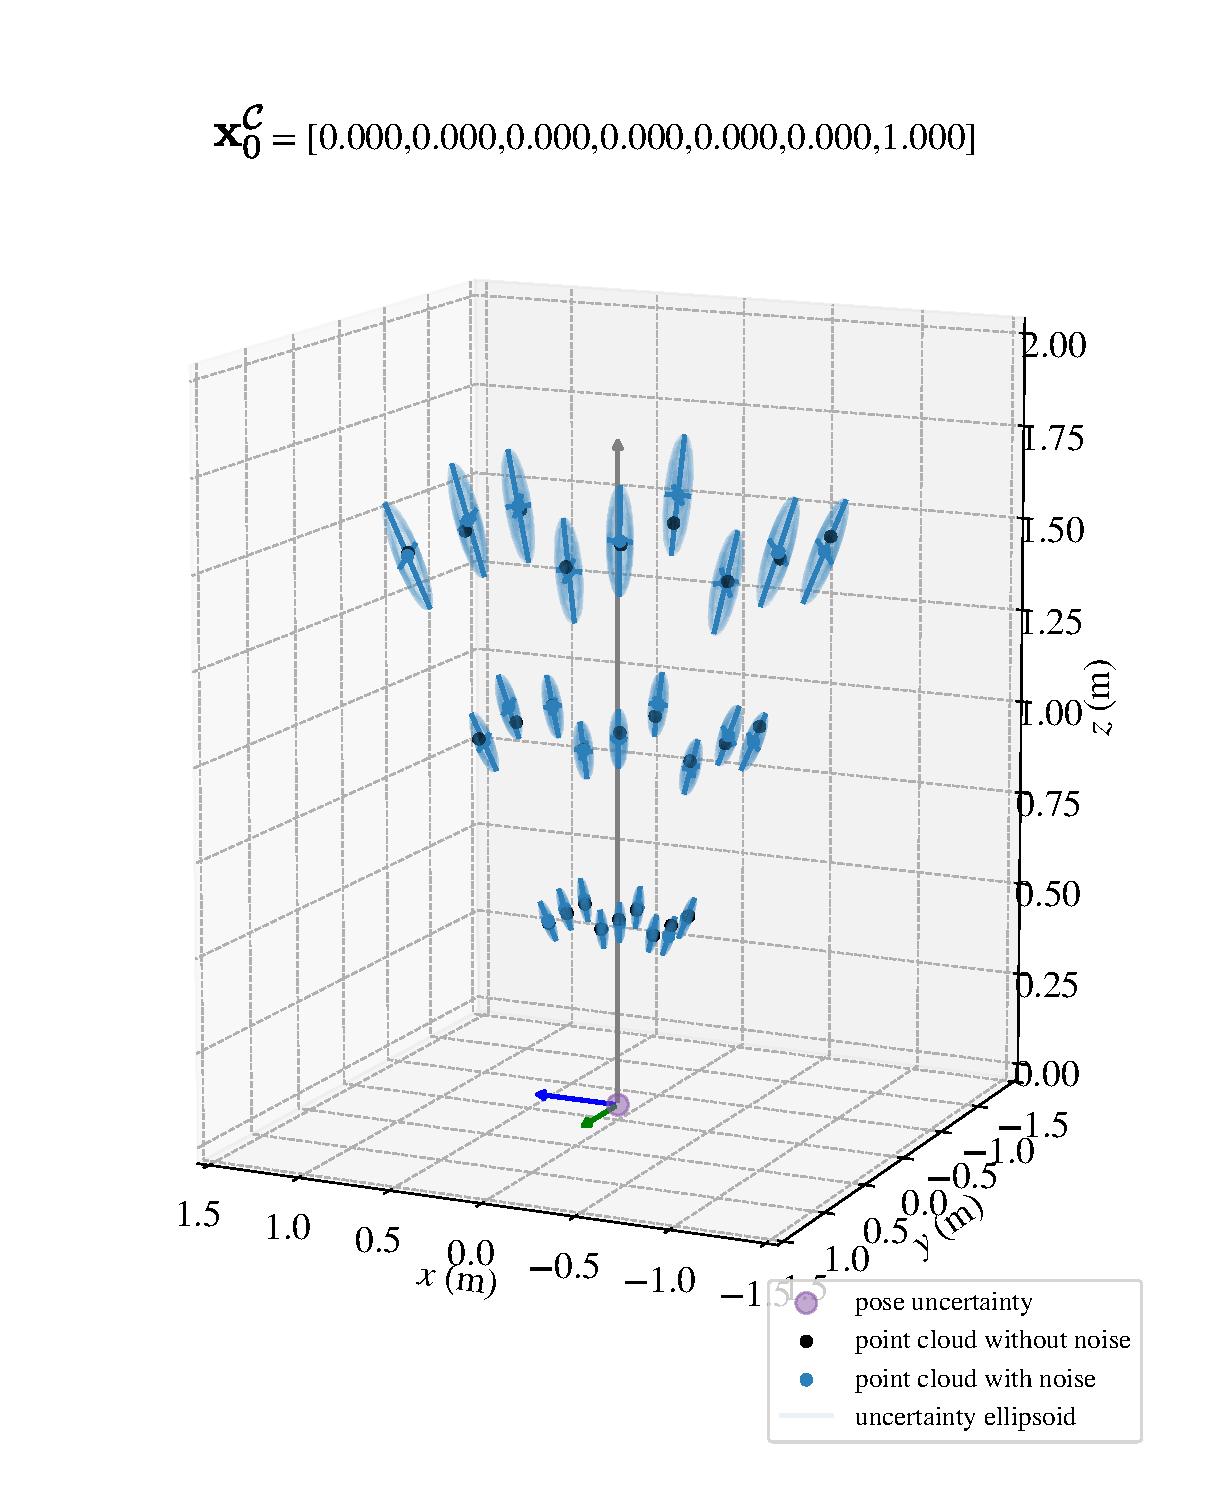
\includegraphics[width=\linewidth,natwidth=640,natheight=640]
  {fig/eva_graphs/sim_at_p0_edit.pdf}
  \caption[Simulation Environment At The Initial Pose]
  {Simulation Environment At The Initial $\mathbf{x}_0^{\mathcal{C}}$ Pose}
	\label{fig:sim_at_p0}
\end{figure}

Figure \ref{fig:sim_at_p0} depicts the environment at its initial pose 
$\mathbf{x}_0^{\mathcal{C}}$.
For the sake of visibility, we only draw a small subset of 3D feature points and scaled the 
confidence ellipses by 10. Notice how the 
volume and orientation of the confidence ellipsoids are situated according to 
the conic ray model.

% Distribution of Point Clouds in 3D at p1
\begin{figure}[H]
  \centering
  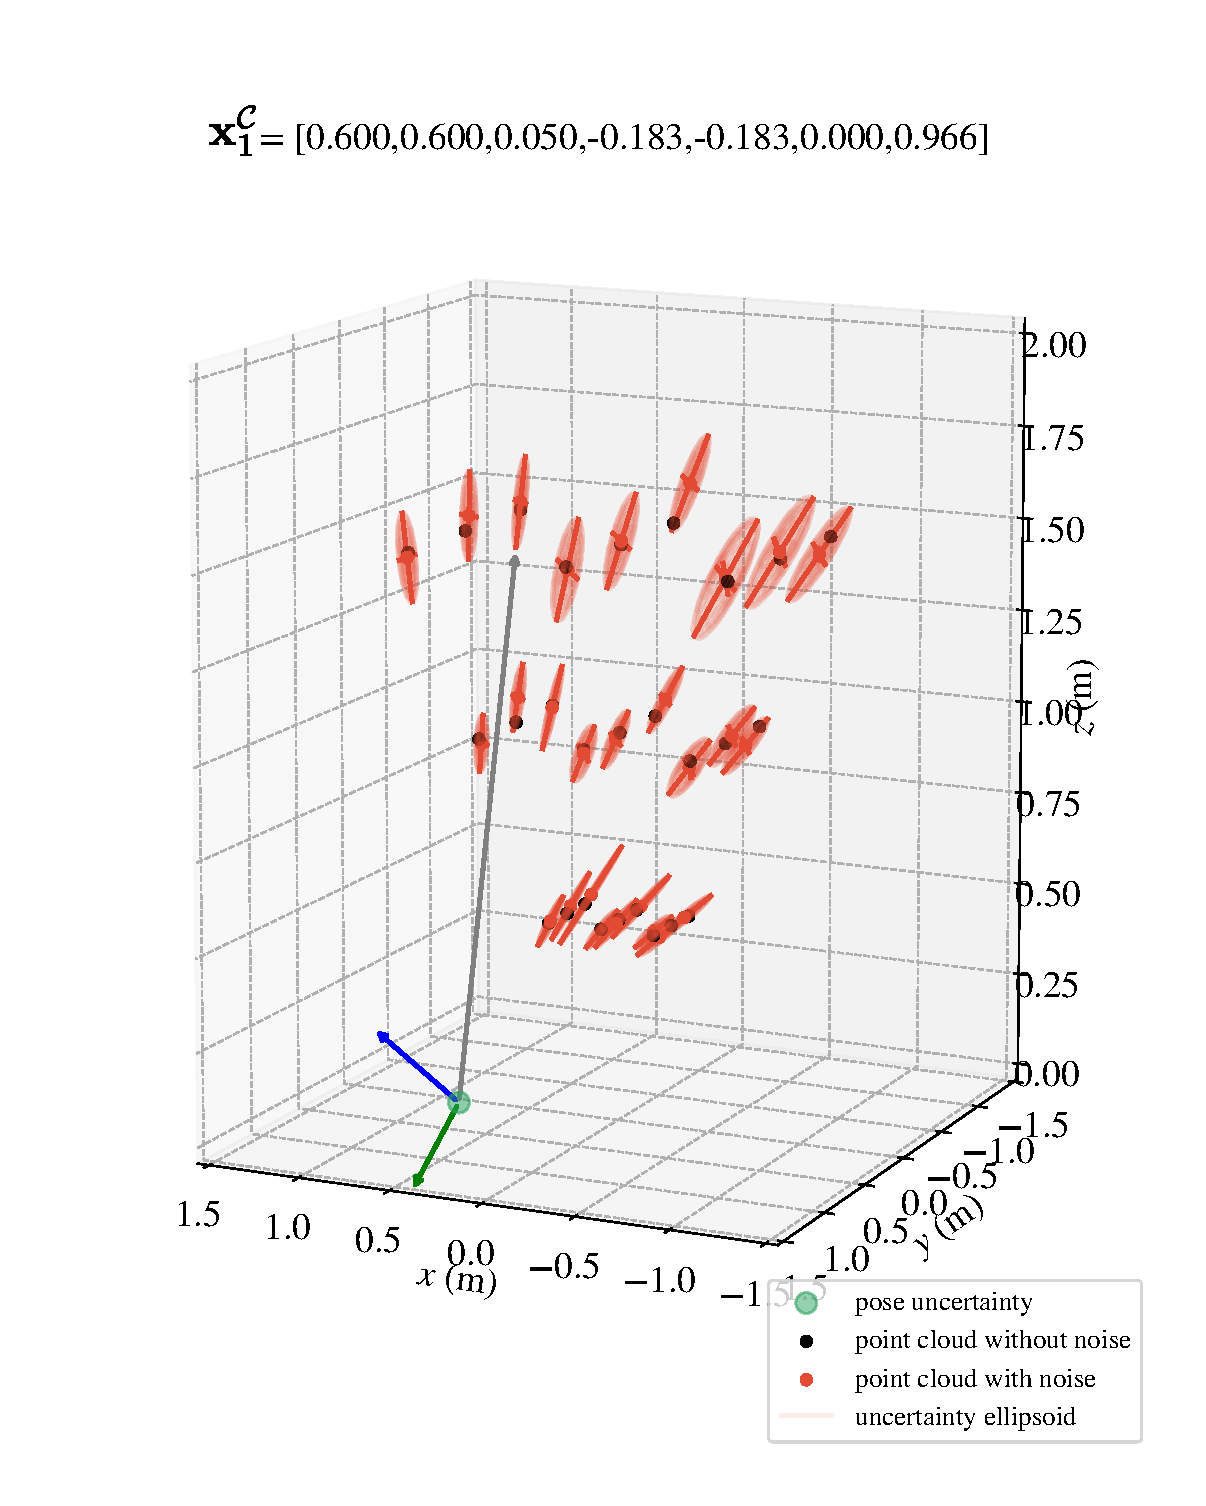
\includegraphics[width=\linewidth,natwidth=640,natheight=640]
  {fig/eva_graphs/sim_at_p1_edit.pdf}
  \caption[Simulation Environment At The Next Pose]
  {Simulation Environment At The Next $\mathbf{x}_1^{\mathcal{C}}$ Pose}
	\label{fig:sim_at_p1}
\end{figure}

Then, we rotate and translate the camera to its next pose 
$\mathbf{x}_0^{\mathcal{C}}$ as shown in Figure 
\ref{fig:sim_at_p1}. Notice how confidence ellipsoids are situated with 
the new camera pose accordingly.


\begin{figure}[H]
  \centering
  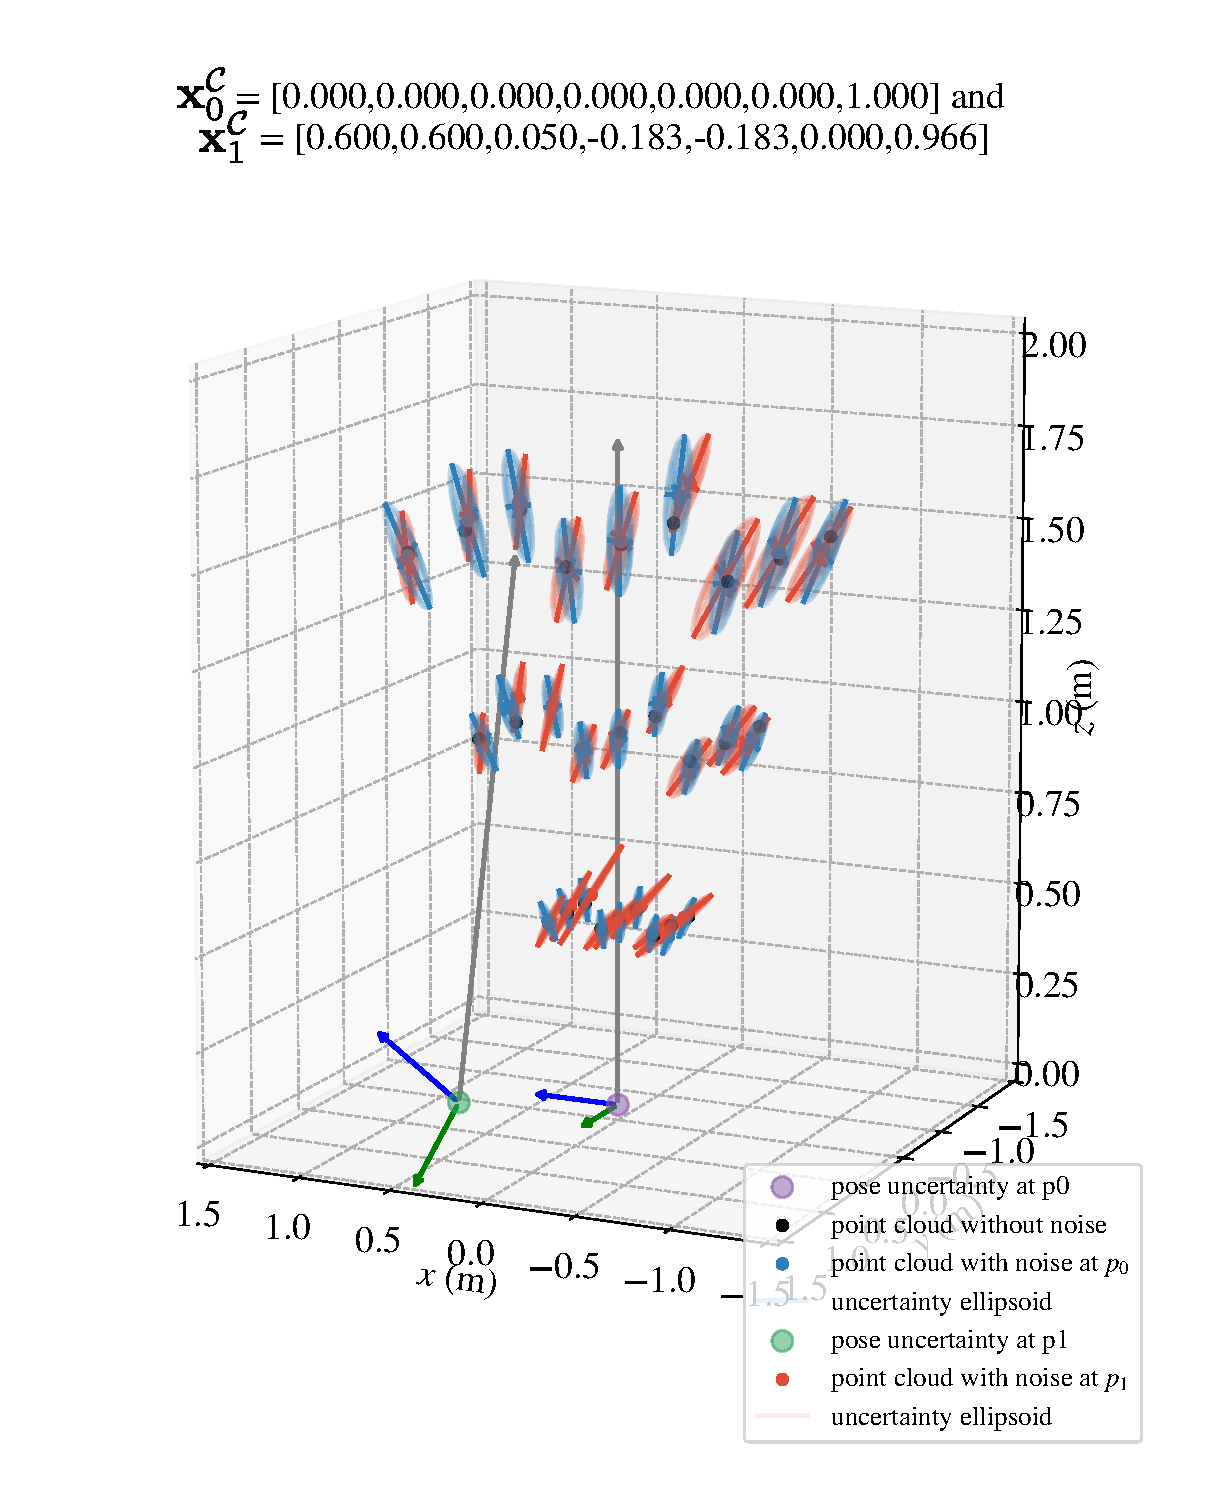
\includegraphics[width=\linewidth,natwidth=640,natheight=640]
  {fig/eva_graphs/sim_at_p0p1_edit.pdf}
  \caption[Simulation Environment At Both Poses]
  {Simulation Environment At Both 
  $\mathbf{x}_0^{\mathcal{C}}$ and $\mathbf{x}_1^{\mathcal{C}}$ Poses}
	\label{fig:sim_at_p0p1}
\end{figure}

Finally, Figure \ref{fig:sim_at_p0p1} shows how confidence ellipsoids 
from both views intersect each other and include the real feature points within 
the intersected space.
Now that we now have everything we need, we can estimate camera transformation 
and its covariance and compare with their original values.

% 4
\subsection{RPE and The Estimated Covariances}

With the simulated data, we run the experiment 1000 times and added random noise on point features. Then, we estimate relative poses $\mathbf{x^*}_{0,1}^{(1:1000)}$ and its covariances $\mathbf{Q}_{\mathbf{tq},0,1}^{(1:1000)}$.  In the end, we calculate RPE with $\Delta=1$ so that we validate whether the RPE lies within the $3\sigma$ bounds for each parameter of the state vector. In this case, $3\sigma$ bounds correspond to a rule of thumb evaluation metric that checks whether the RPE are bounded with 99.7\% probability.

% Translation RPE with 3 sigma 
\begin{figure}[H]
  \centering
  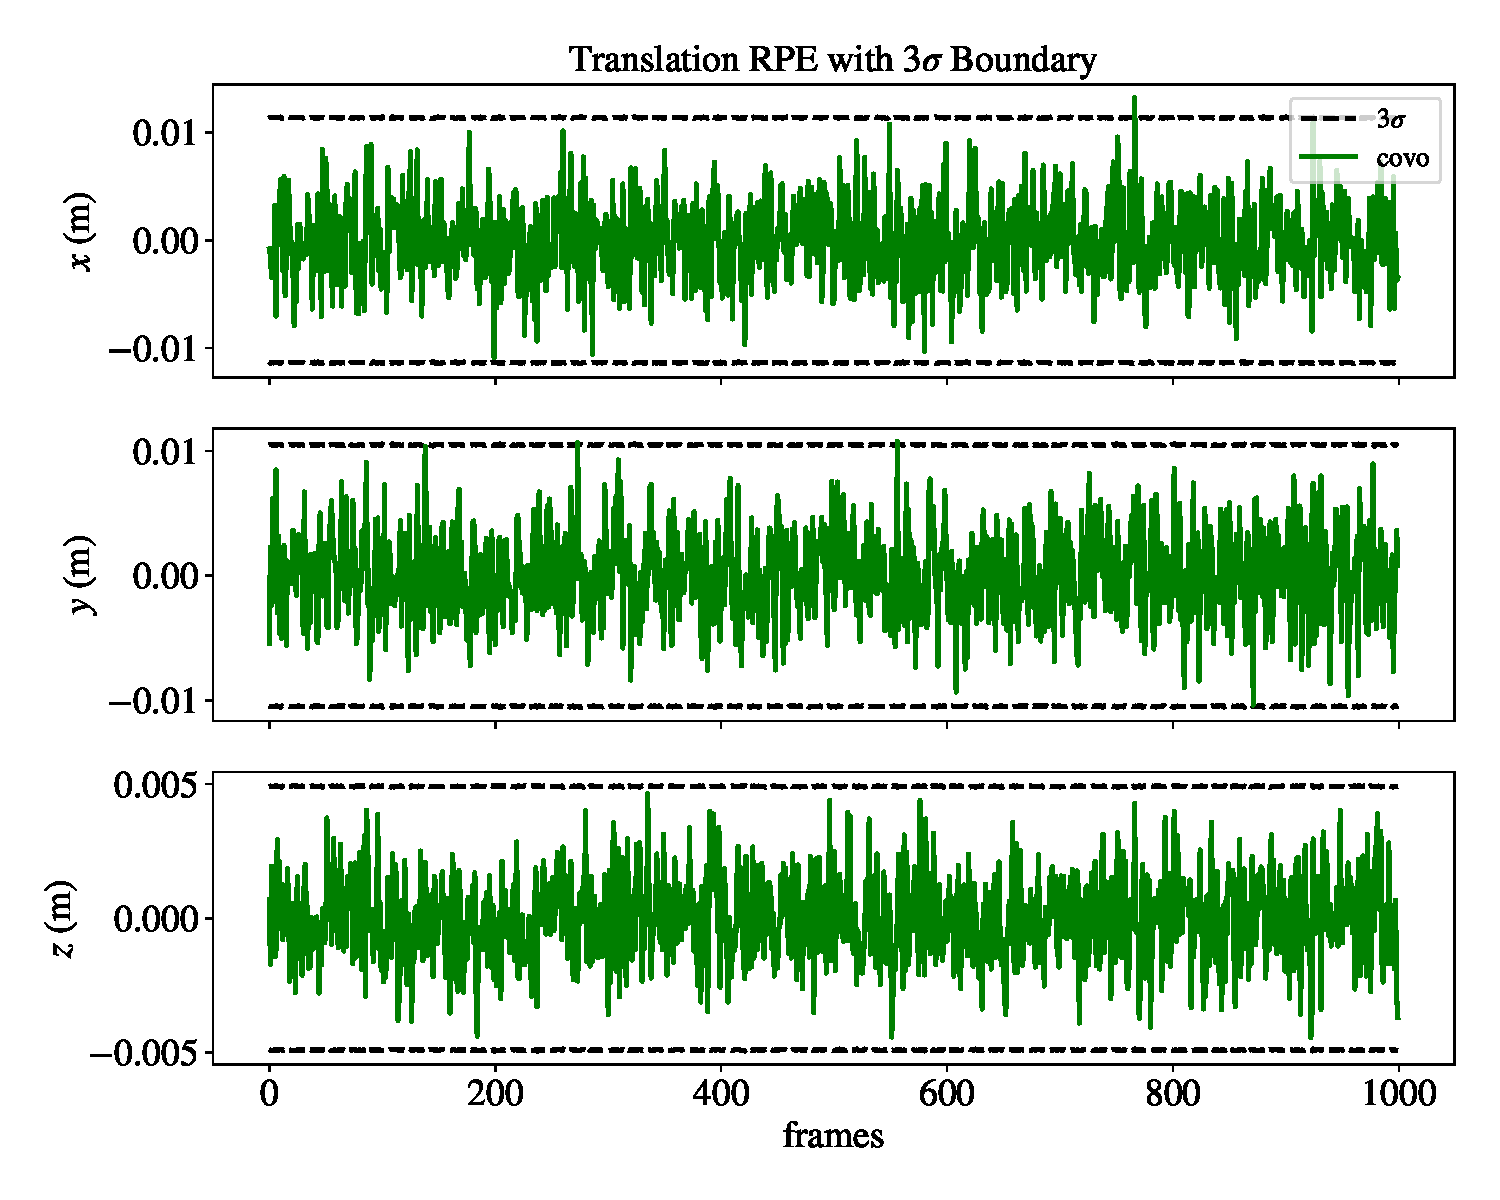
\includegraphics[width=0.8\linewidth,natwidth=640,natheight=640]
  {fig/eva_graphs/synt_trans_rpe_3sigma.pdf}
  \caption{Translational RPE in Simulation Environment}
  \label{fig:synt_trans_rpe_3sigma}
\end{figure}

As seen in Figure \ref{fig:synt_trans_rpe_3sigma}, the translational RPE 
are bounded with except 2 predictions which is statistically 
acceptable. 

% Rotation RPE with 3 sigma 
\begin{figure}[H]
  \centering
  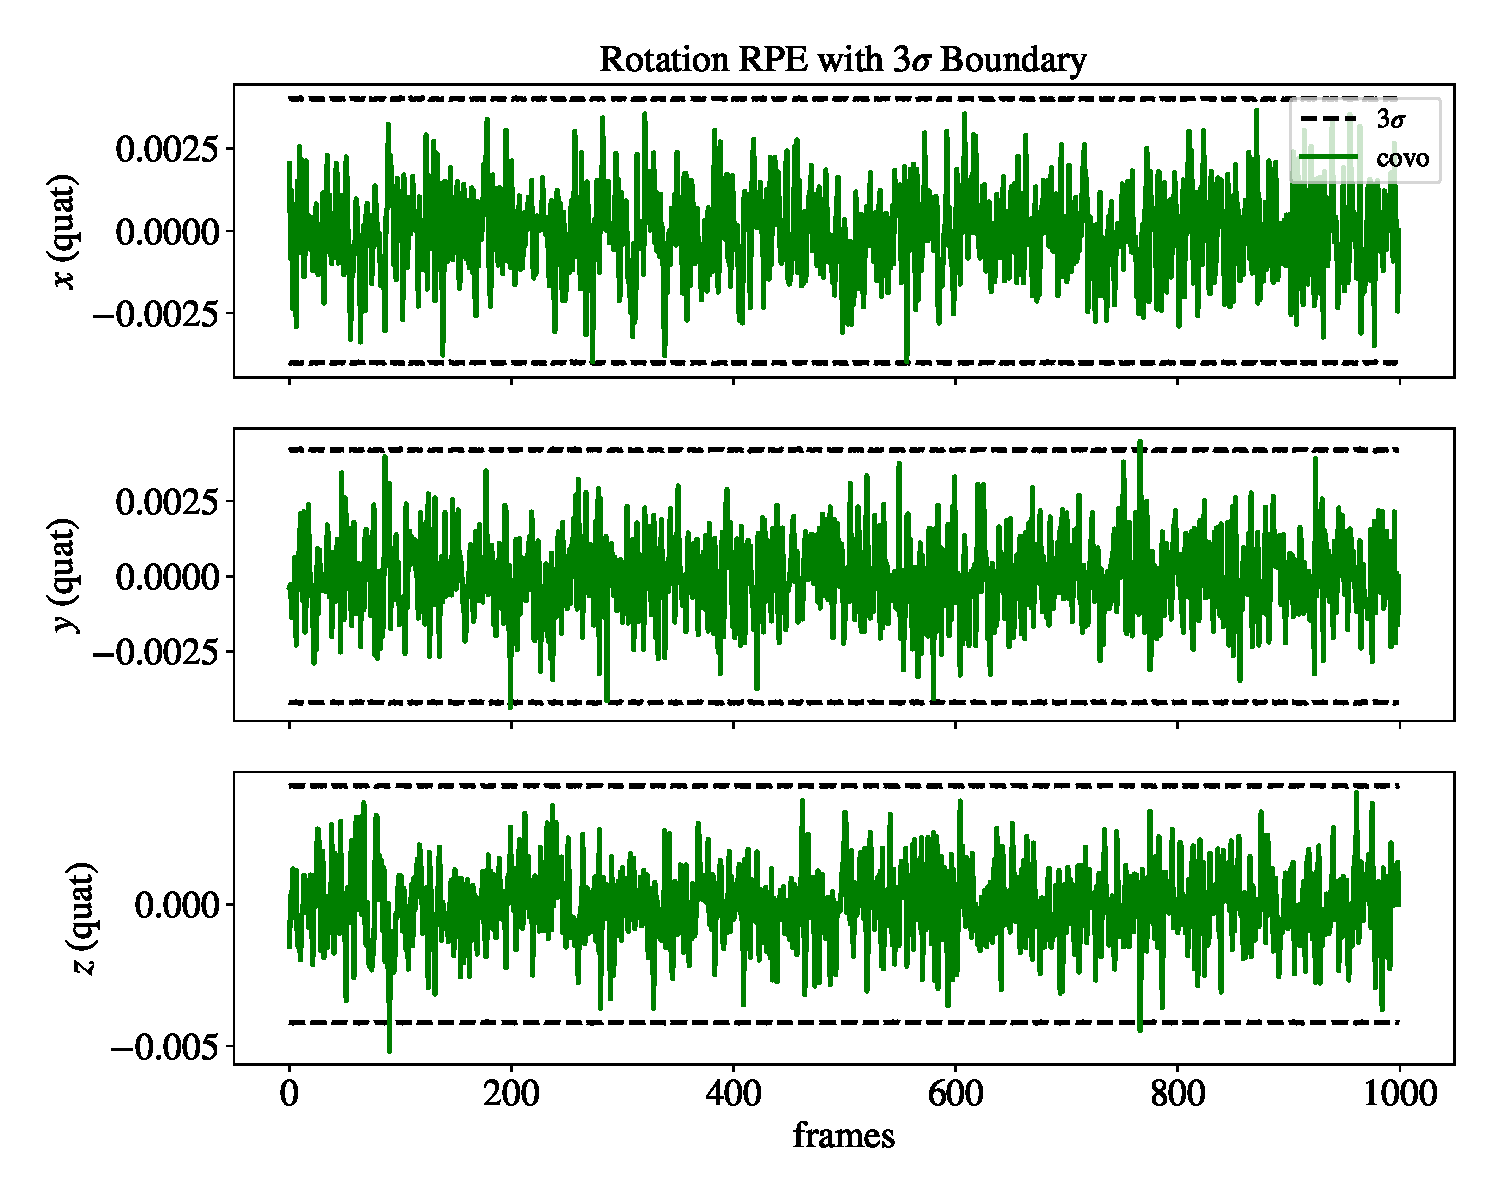
\includegraphics[width=0.8\linewidth,natwidth=640,natheight=640]
  {fig/eva_graphs/synt_rot_rpe_3sigma.pdf}
  \caption{Rotational RPE in Simulation Environment}
	\label{fig:synt_rot_rpe_3sigma}
\end{figure}

The same behavior is observed for the rotation as seen in Figure 
\ref{fig:synt_rot_rpe_3sigma}. It indicates that the propagated covariances of 
the estimated poses based on the proposed model produce statistically 
acceptable covariances with simulated data if $3\sigma$ bounds are 
considered.  What we also noticed that the majority of the RPE are beyond the 
$1\sigma$ bounds, which is not acceptable since $1\sigma$ corresponds to 68\% 
probability.  In other words, we expected that 68\% of the RPE must be bounded 
with $1\sigma$, which does not hold in our case. This is because we introduce 
a non-linearity with the projection function. That means the noise is not 
Gaussian anymore when we propagate point feature covariances 
$\mathbf{Q}_{\mathbf{xyz},0,1}$ from its disparity space 
$\mathbf{Q}_{\mathbf{uvd},0,1}$ with the non-linear error propagation which is 
the approximated with the first-order Taylor expansion $\mathbf{J_{bp}}$ (see 
notation \eqref{eq:cov_xyz_prop}).  However, $\sigma$ bounds evaluations 
itself is not enough to prove estimator's credibility. Thus, further 
evaluations are done with NEES.

% 3
\subsection{Evaluation of Estimated Covariances}

Even though $\sigma$ bounds confirm that our algorithm provides consistent 
pose estimation given RPE is bounded with $3\sigma$, we need to check whether 
the covariance of the estimated pose is being too optimistic or not since it 
fails at $1\sigma$.  Hence, we run our simulation as described at the 
beginning of this section again.  Then, we calculate ANEES; i.e., 15.64 for 
translation and 15.72 for rotation.  Also, the results are illustrated in 
Figure \ref{fig:test_hist_nees_1}.


\begin{figure}[H] \begin{tabular}{ccc} \centering \subcaptionbox{NEES}{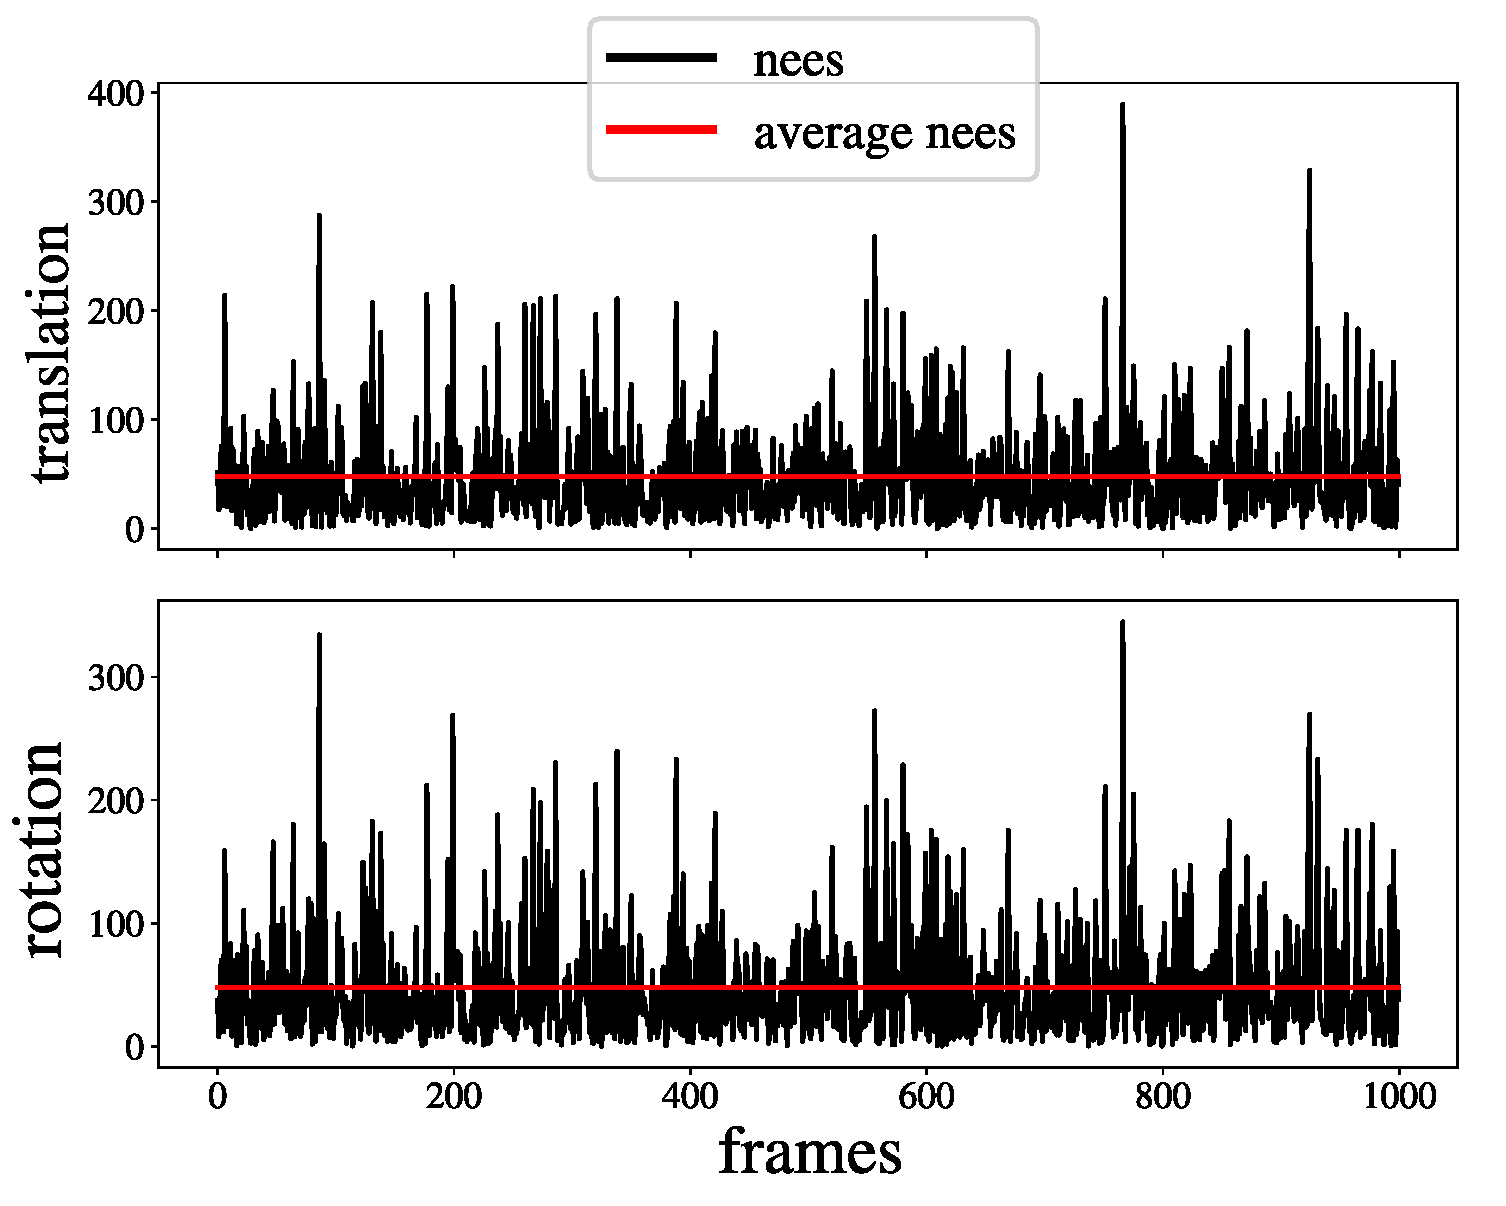
\includegraphics[width = 0.55\linewidth]{fig/eva_graphs/synt_nees.pdf}} & \subcaptionbox{Histogram of NEES}{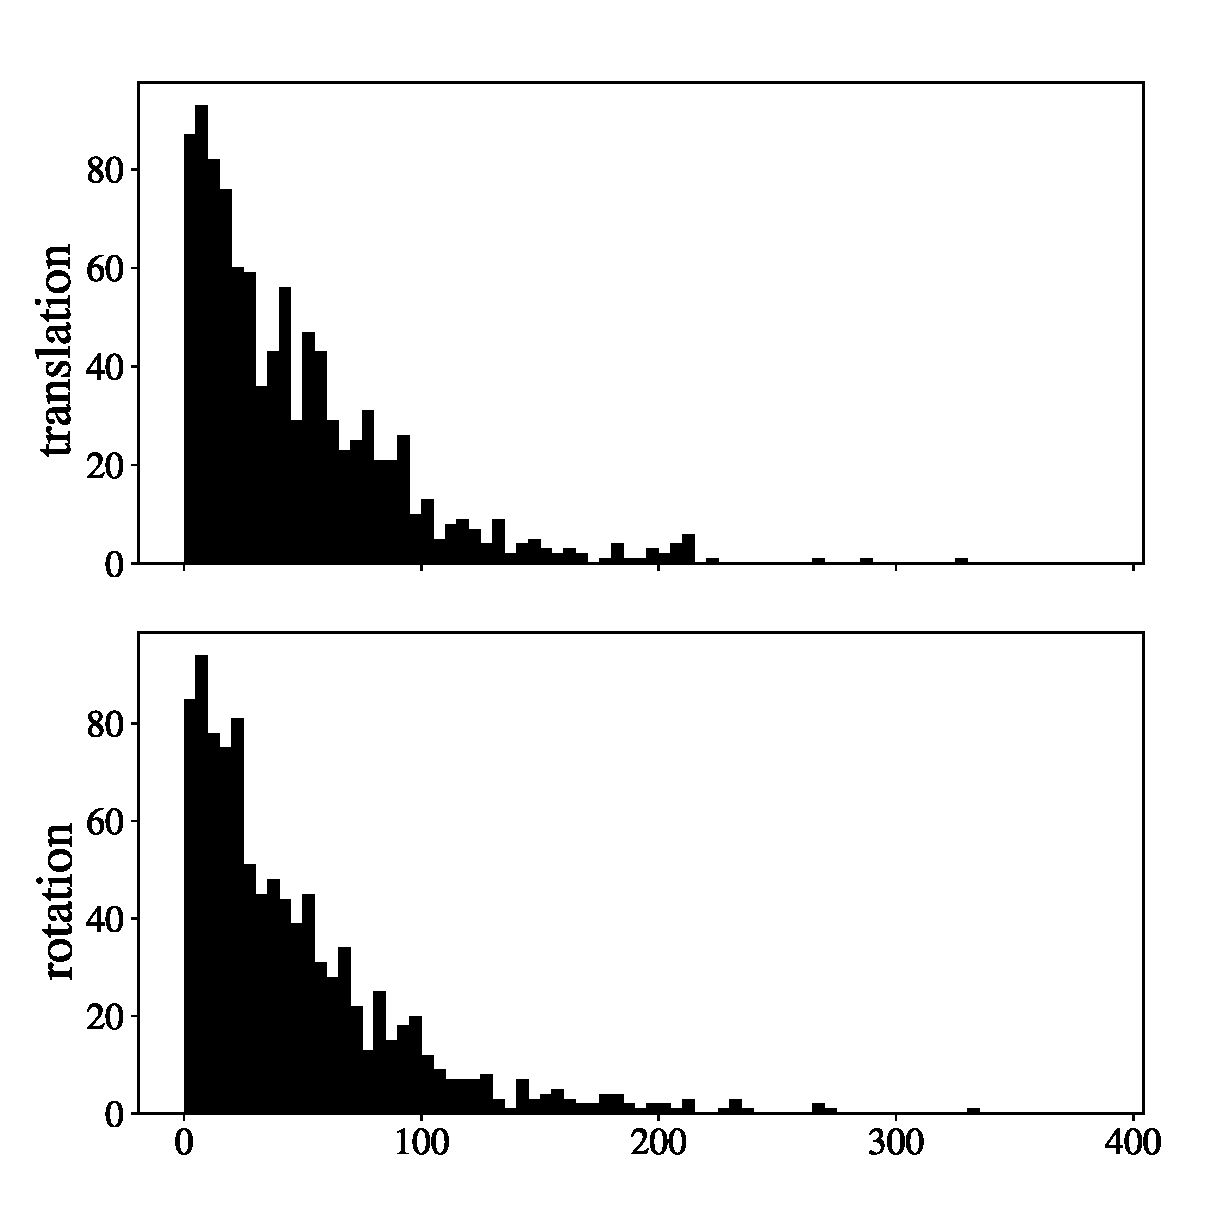
\includegraphics[width = 0.40\linewidth]{fig/eva_graphs/synt_hist_nees.pdf}} \end{tabular} \caption{NEES For Simulated Data Without $\phi$ Scaling Factor} \label{fig:test_hist_nees_1} \end{figure}


These results show that the estimator is not consistent according to the ANEES 
analysis. This is because the projection operation introduces non-linearity to 
the system as mentioned before.  This linearization process does not work well 
with large noises, i.e., the pixel noise: $\sigma_u=8, \sigma_v=8$, and the 
depth noise: $\sigma_Z$ especially for the features that get larger with the 
range.  Moreover, we run multiples test scenarios where the pixel uncertainty 
was kept small such as $0<\sigma_u<2$ and $0<\sigma_v<2$, and the features are 
located under $z<1m$ range. In this case, we approximation works and the ANEES 
decreases below $3$ for both translation and rotation, which is the acceptance 
threshold for a consistent estimator.  In this perspective, 
\parencite[see][395--397]{Shalom2001} suggest a couple of heuristic methods to 
make the estimator consistent.  Among them, we apply multiplication of 
estimated covariance $\mathbf{Q}_{\mathbf{tq}, k,k+1}$ by scaling factor 
$\phi$ after optimization.

\begin{figure}[H] \begin{tabular}{ccc} \centering \subcaptionbox{NEES}{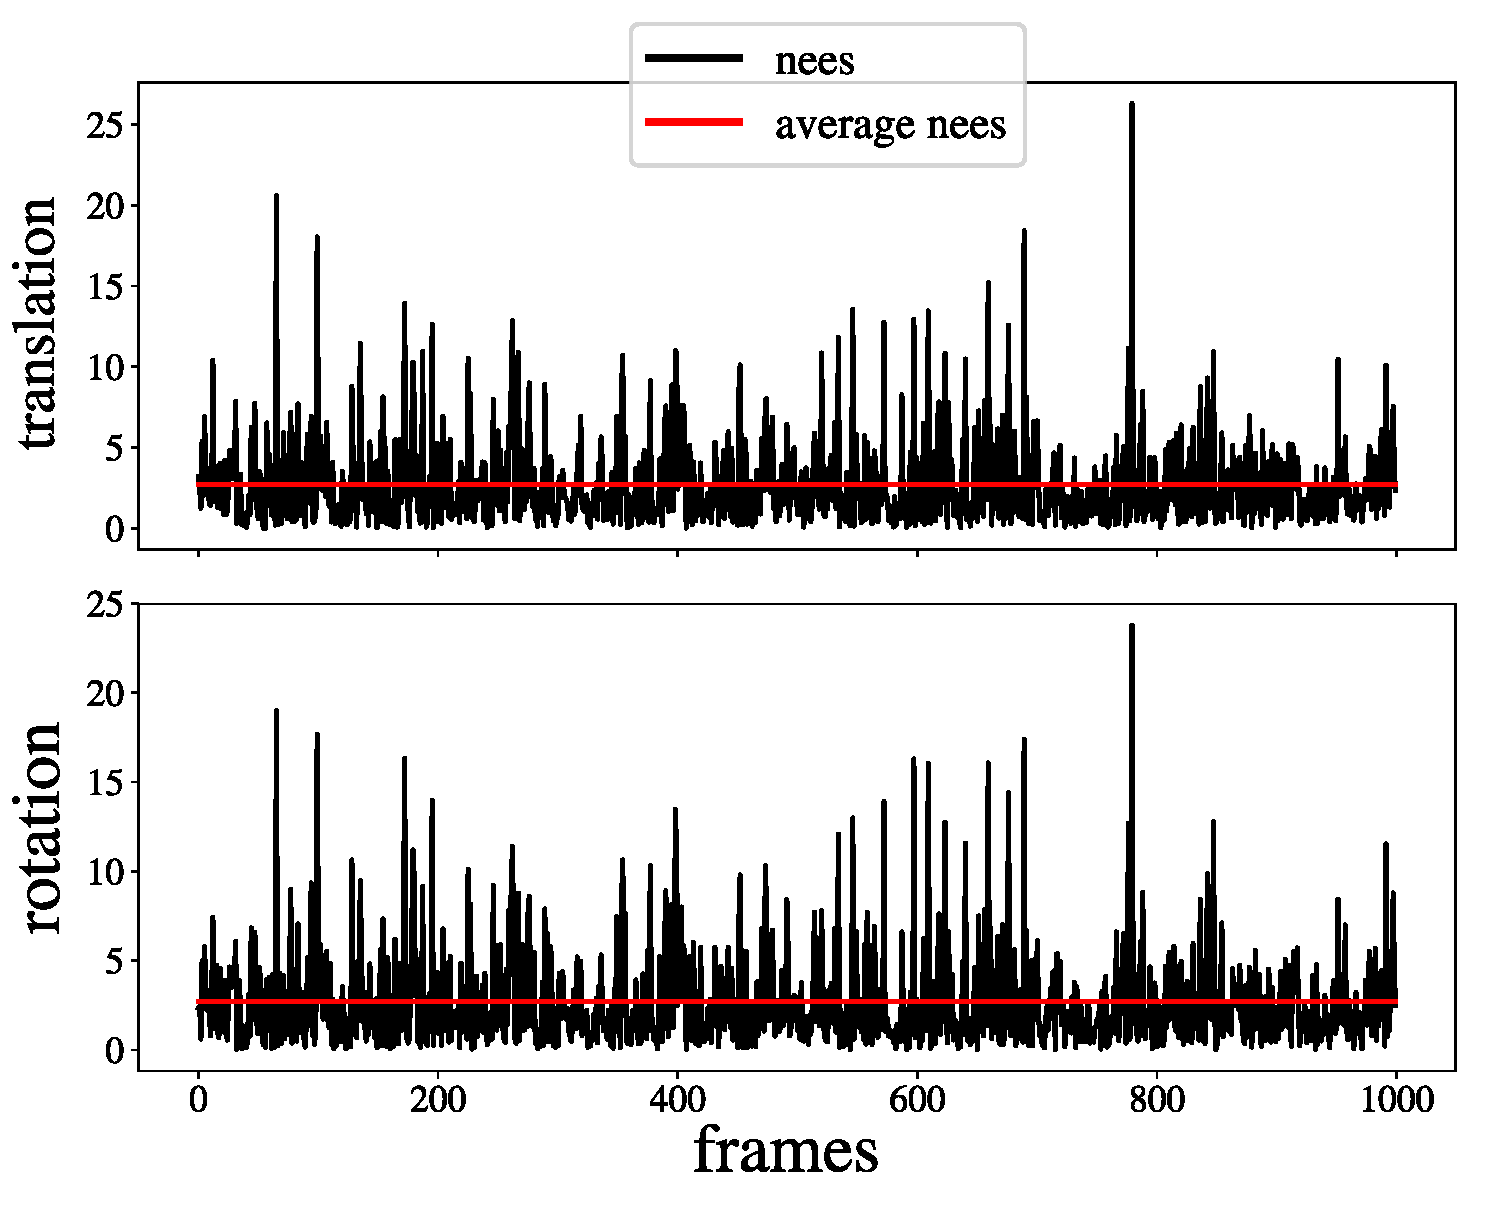
\includegraphics[width = 0.55\linewidth]{fig/eva_graphs/synt_nees_2.pdf}} & \subcaptionbox{Histogram of NEES}{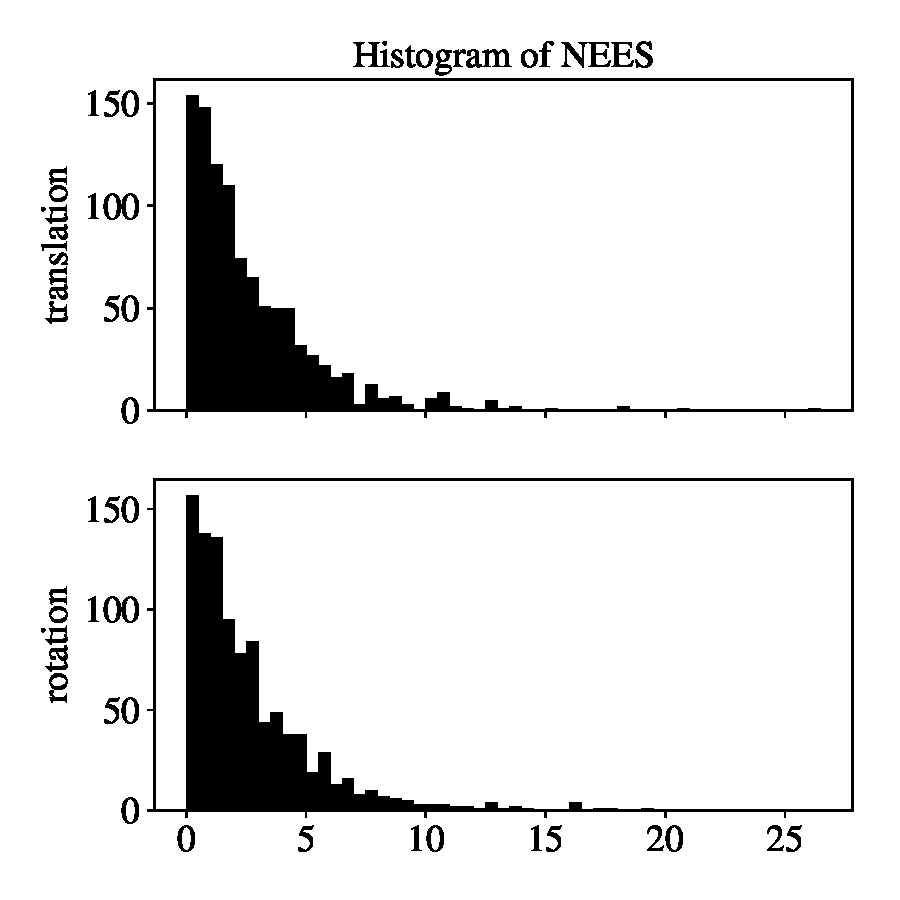
\includegraphics[width = 0.40\linewidth]{fig/eva_graphs/synt_hist_nees_2.pdf}} \end{tabular} \caption{NEES For Simulated Data With $\phi=4^2$ Scaling Factor} \label{fig:test_hist_nees_2} \end{figure}

For our initial test setup which extensively described in Section 
\ref{sc_sim_env}, we find out that ANEES for translation and rotation becomes 
2.7 and 2.69, respectively when taking $\phi=4^2$ and the results are shown in 
Figure \ref{fig:test_hist_nees_2}.  Therefore, the scaling factor can be 
accepted as we consider the estimator to be consistent with this setup.  The 
reason we take this setup along with all empiric parameters in the simulation 
is that we want to create an environment that covers the possible worst case 
scenarios in the real-world dataset.  We will explain why we specifically set 
$\sigma_u=8$ and $\sigma_v=8$ after analyzing the effect of pseudo inliers in 
the following Section \ref{sc_pseudo_inliers}. 


\section{TUM RGB-D Dataset}

TUM dataset by \parencite{Sturm2012a} provides an extensive benchmark 
capability for RGB-D based Visual SLAM or VO systems. It consists of datasets 
that are collected in two different indoor environments; i.e., fr1 refers to 
datasets collected in an office $(6\times 6 m^2)$ and fr2 is collected in an 
open spaced garage $(10\times 12m^2)$. In our experiments, we choose a subset 
of datasets that are mainly suitable for VO and has sufficient texture on the 
images.  The selected datasets are given in Table \ref{tb:tum_dataset}.  
Besides, calibration parameters of RGB and depth images are validated by the 
time-synchronized ground truth measurements recorded by a motion capture 
system.

\begin{table}
\begin{center}
  \begin{tabular}{lccc}
    \hline
    Dataset & Duration & Avg. Trans. & Avg. Rot.\\
     Name & [s] & Vel. [m/s] & Vel. [deg/s]\\
    \hline
    fr1 xyz   & 30 & 0.24 & 8.92\\
    fr1 rpy   & 28 & 0.06 & 50.15\\
    fr1 room  & 49 & 0.33 & 29.88\\
    fr1 360   & 29 & 0.21 & 41.60\\
    fr1 desk  & 23 & 0.41 & 23.33\\
    fr1 desk2 & 25 & 0.43 & 29.31\\
    fr2 desk  & 99 & 0.19 & 6.34\\
    \hline
  \end{tabular}
\end{center}
  \caption{List of Chosen TUM RGB-D Datasets}
  \label{tb:tum_dataset}
\end{table}

Before we use these datasets to validate 
our relative pose estimation and its covariance, 
we are going to investigate the effect of pseudo inliers that 
exist in our feature matches even after applying RANSAC. 

\subsection{Discovering the Effect of Pseudo Inliers on Pixel Uncertainty}\label{sc_pseudo_inliers}

As discussed earlier in Section \ref{sb_sc_pixel_uncertainty}, the pixel 
uncertainty caused by quantization operation is treated as a half pixel.  
Nevertheless, this error is itself not sufficient when choosing a standard 
deviation of pixel noise for feature covariances to be propagated through the 
equation \eqref{eq:cov_xyz_prop}. Remember that we still had outliers in 
feature matching even after applying RANSAC, which we call them as pseudo 
inliers. We proposed to treat them as inliers in the condition that they will 
increase the pixel uncertainty.  Moreover, we expected that RANSAC would bound 
these pseudo inliers, which can utilize them as pixel noise. Thus, we are 
interested in determining the boundaries of the pseudo inliers.  Since we have 
TUM RGB-D dataset and the ground truth measurements, we can calculate the 
pixel error of the pseudo inliers by aligning feature matches with 
transformation information from ground truth.


\begin{figure}[H] \makebox[\textwidth][c]{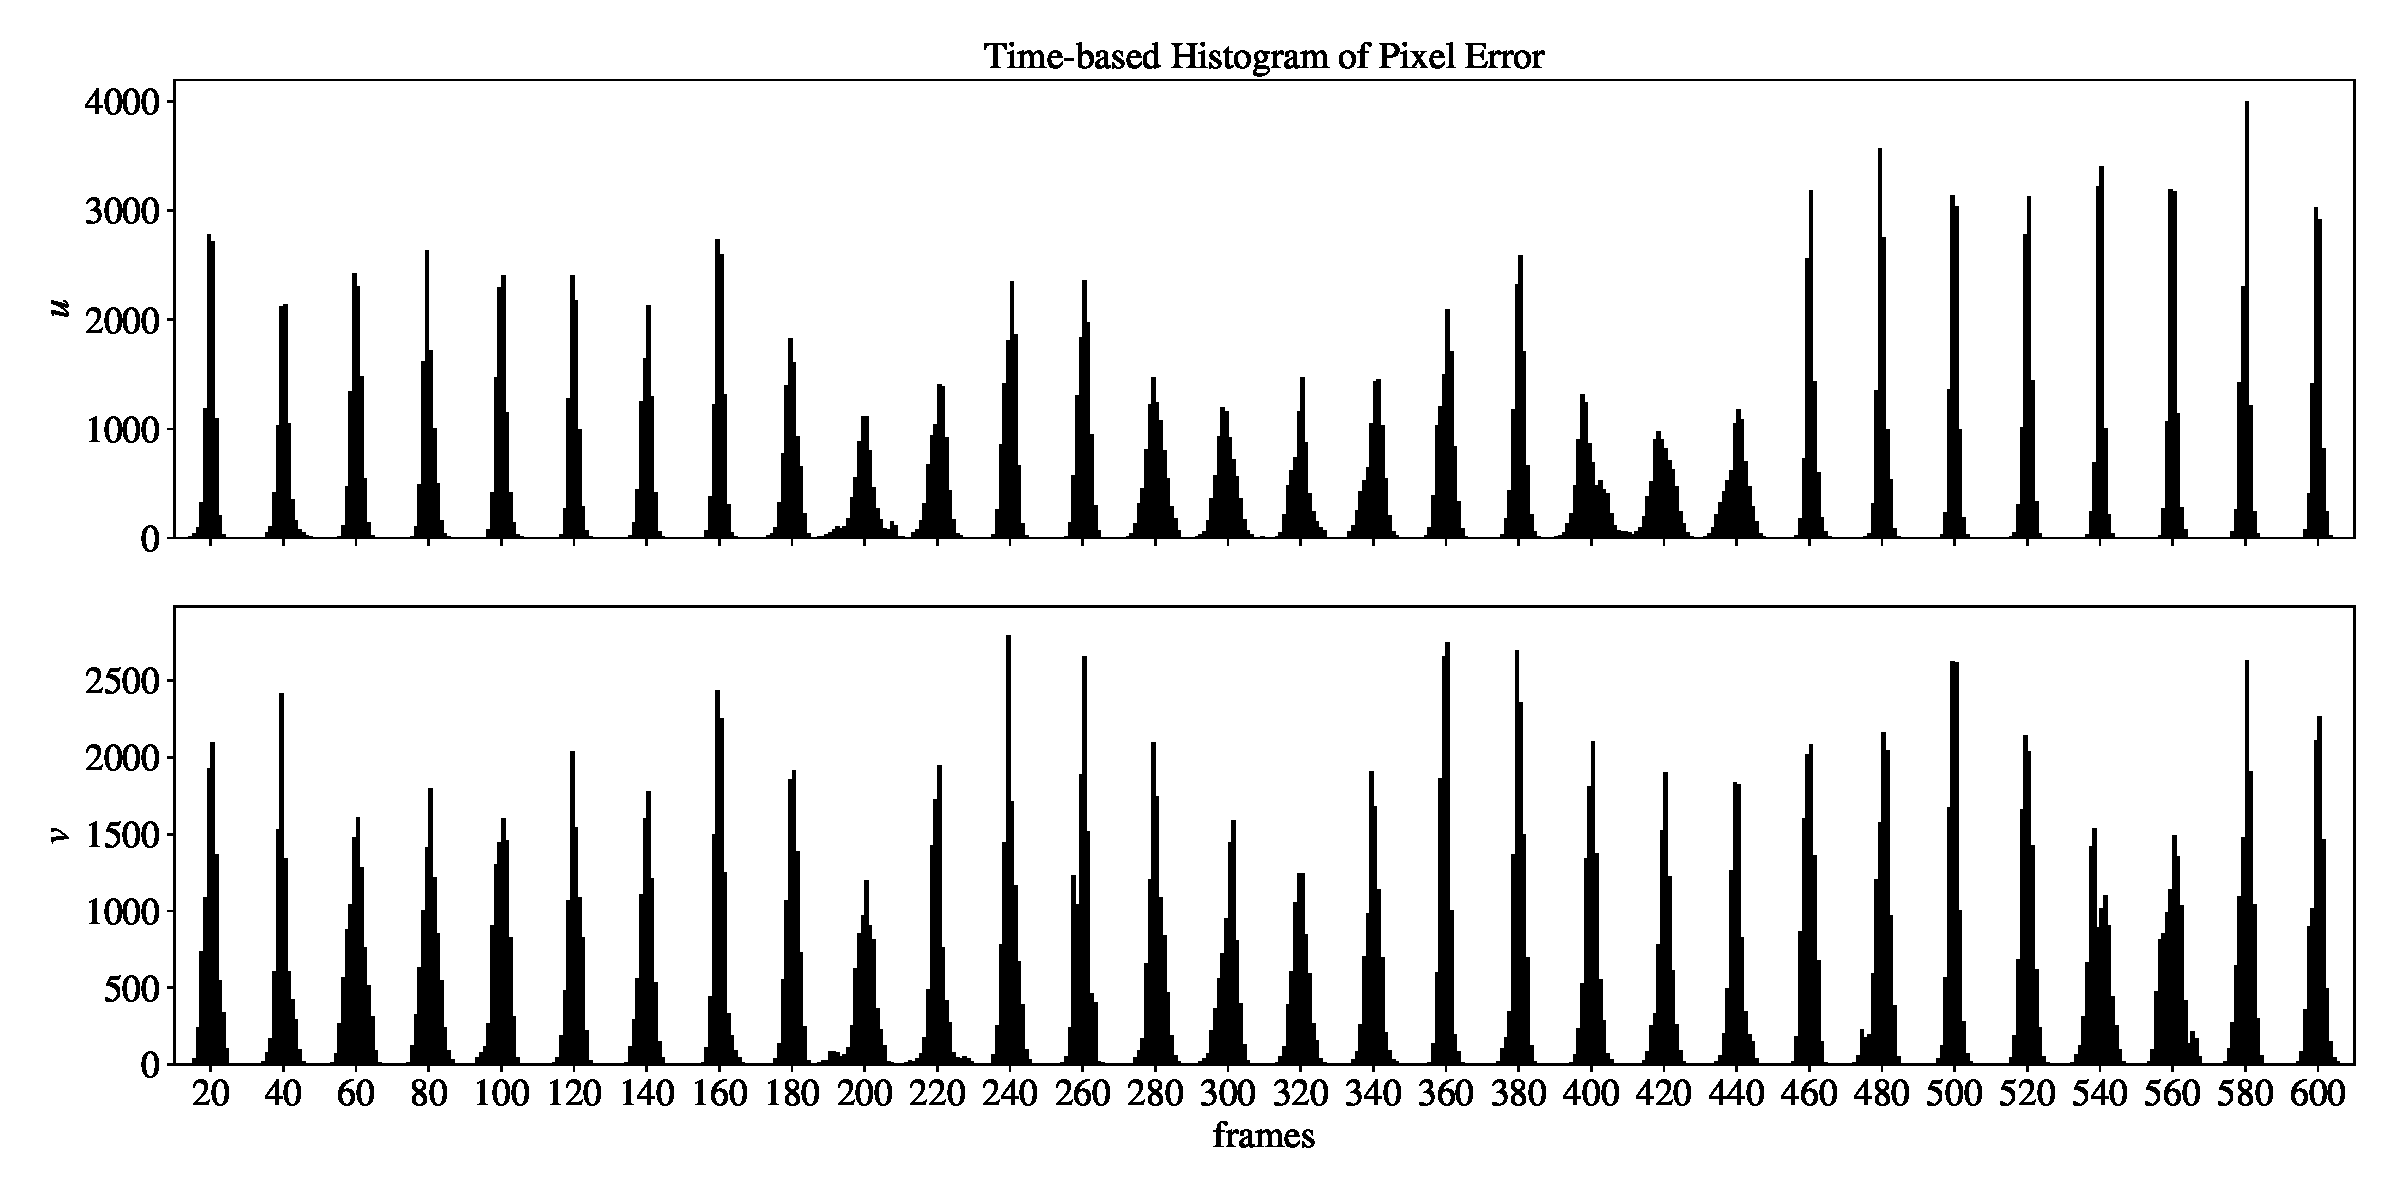
\includegraphics[width=1.4\linewidth,natwidth=640,natheight=640] {fig/eva_graphs/tum_fr1_xyz_tbased_hist_uv_err.pdf}} \caption[Time-based Histogram of Pixel Errors]{ This illustration shows how the pixel error distances are distibuted along the trajectory. Note that we grouped the errors every 20 frames.} \label{fig:time_based_hist_pix_err} \end{figure}

To be more specific, let's remind ourselves with the CoVO pipeline.  To find 
the pixel error caused by pseudo inliers, we run our CoVO algorithm up until 
the optimization part at which we estimate the 
$\mathbf{x^*}_{k,k+1}(=\mathbf{T^*}_{k,k+1})$ transformation information.  At 
this point, we already have feature matches that include pseudo inliers.  Now, 
instead of estimating the transformation with LM algorithm, we can rotate 
and translate $\mathbf{u}^{(k,1:m)}$ features from $k^{th}$ frame towards 
$k+1^{th}$ frame and save them as $\mathbf{\hat{u}}^{(k+1,1:m)}$.  In an ideal 
case, we expect transformed $\mathbf{\hat{u}}^{(k+1,1:m)}$ features and 
measured $\mathbf{u}^{(k+1,1:m)}$ features to be aligned closely such that the 
error distances between them are maximum a half pixel.  Regardless, the error 
distance for some matches will be greater than a half pixel due to the pseudo 
inliers as we are operating on a real-world dataset.  As a result, we can use 
this test case to identify the pixel error distance caused by the pseudo 
inliers.  We can now apply to every consecutive frame of the whole 
trajectory.  Thus, we illustrate the results in a time-based scheme to observe 
how the pixel error changes throughout the trajectory. The illustration 
gathered by 'fr1 xyz' dataset is given in Figure 
\ref{fig:time_based_hist_pix_err}.  As seen, the pixel distance error is 
distributed as Gaussian and its standard deviation changes over the 
trajectory.  To see how the standard deviation changes clearly, we draw the 
time-based standard deviation of the pixel errors in Figure 
\ref{fig:time_based_std_pix_err}.


\begin{figure}[H] \centering 
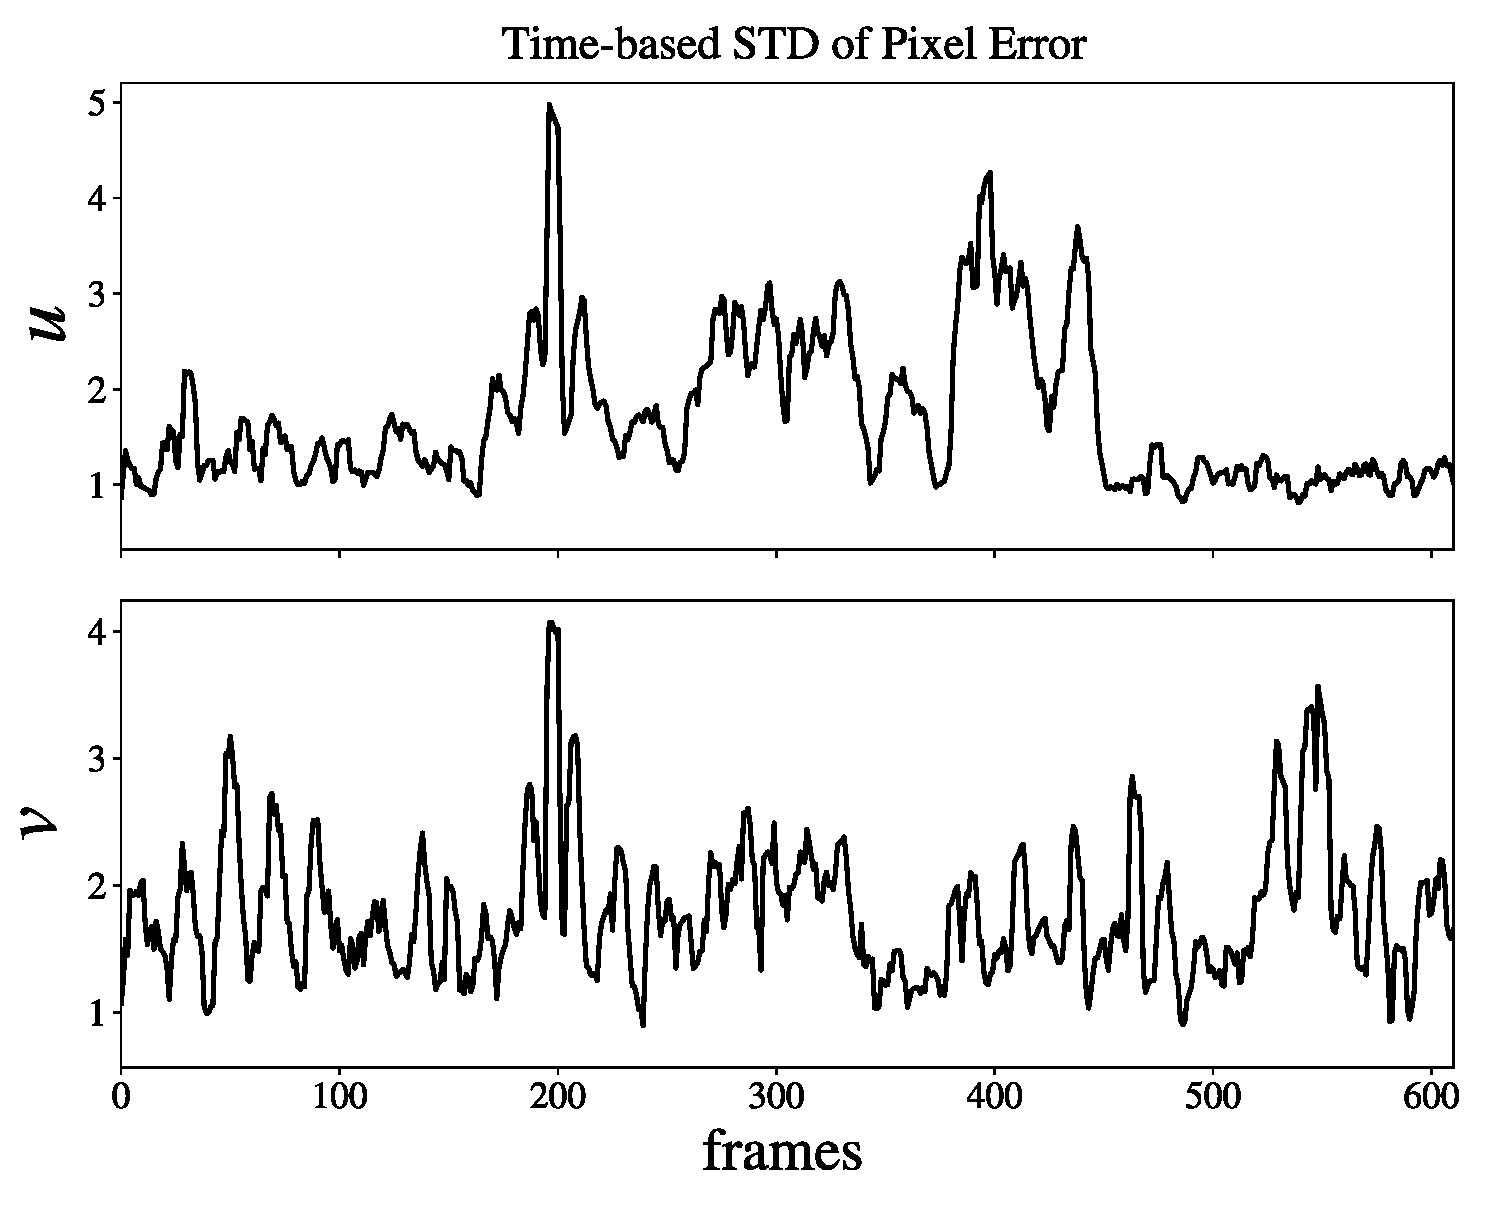
\includegraphics[width=0.8\linewidth,natwidth=640,natheight=640] 
{fig/eva_graphs/tum_fr1_xyz_tbased_uv_err_std.pdf} \caption[The Standard 
Deviations of Pixel Errors] {As seen in the previous figure, the pixel errors 
were distributed Gaussian but varying with time. Thus, this figure is drawn to 
see how the standard deviation of these distributions changes throughout the 
trajectory more clearly }\label{fig:time_based_std_pix_err} \end{figure}

Because we want to cover as many corner cases as possible, we run the test 
over many datasets so that we can find the largest standard deviation. To see 
all datasets' results, we take the time-based standard deviation results which 
we use to draw Figure \ref{fig:time_based_std_pix_err} and illustrate with a 
boxplot.  All the standard deviations of the pixel error from six different 
datasets are given in in Figure \ref{fig:boxplot_time_based_std_all_datasets}.


\begin{figure}[H]
\begin{tabular}{ccc}
\centering
\subcaptionbox{fr1 xyz}{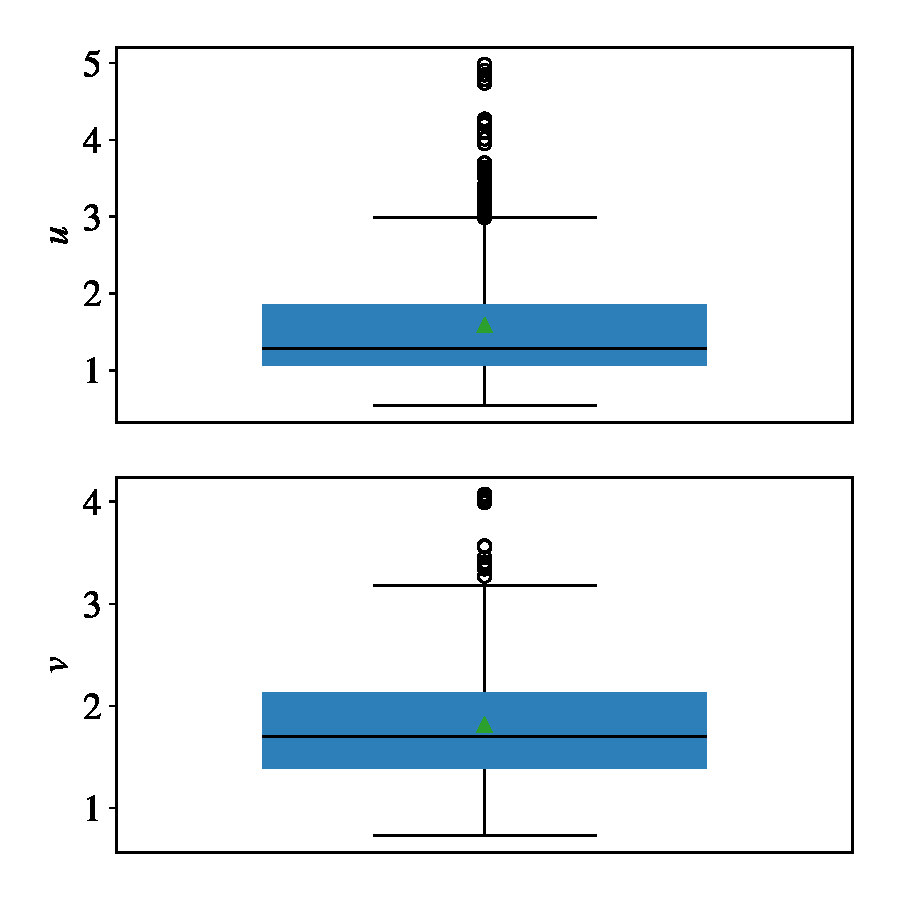
\includegraphics[width = 0.3\linewidth]{fig/eva_graphs/boxplot_tbased_uv_err_std_fr1_xyz.pdf}} &
\subcaptionbox{fr1 rpy}{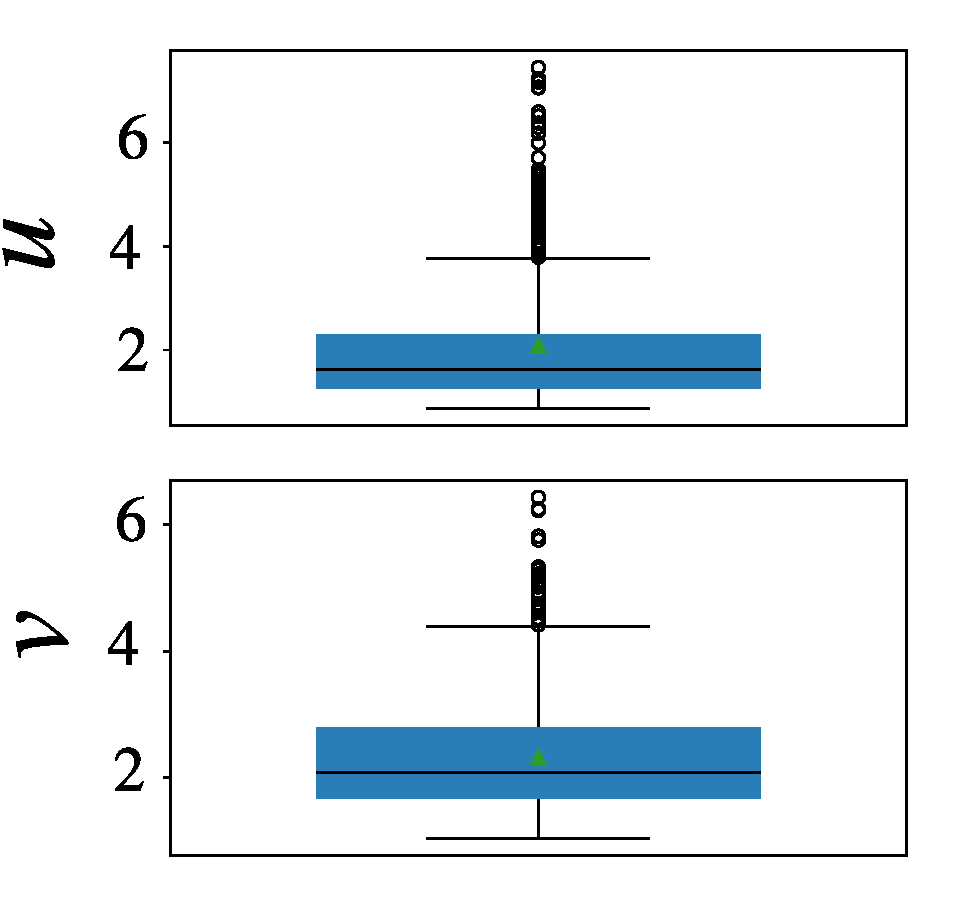
\includegraphics[width = 0.3\linewidth]{fig/eva_graphs/boxplot_tbased_uv_err_std_fr1_rpy.pdf}} &
\subcaptionbox{fr1 room}{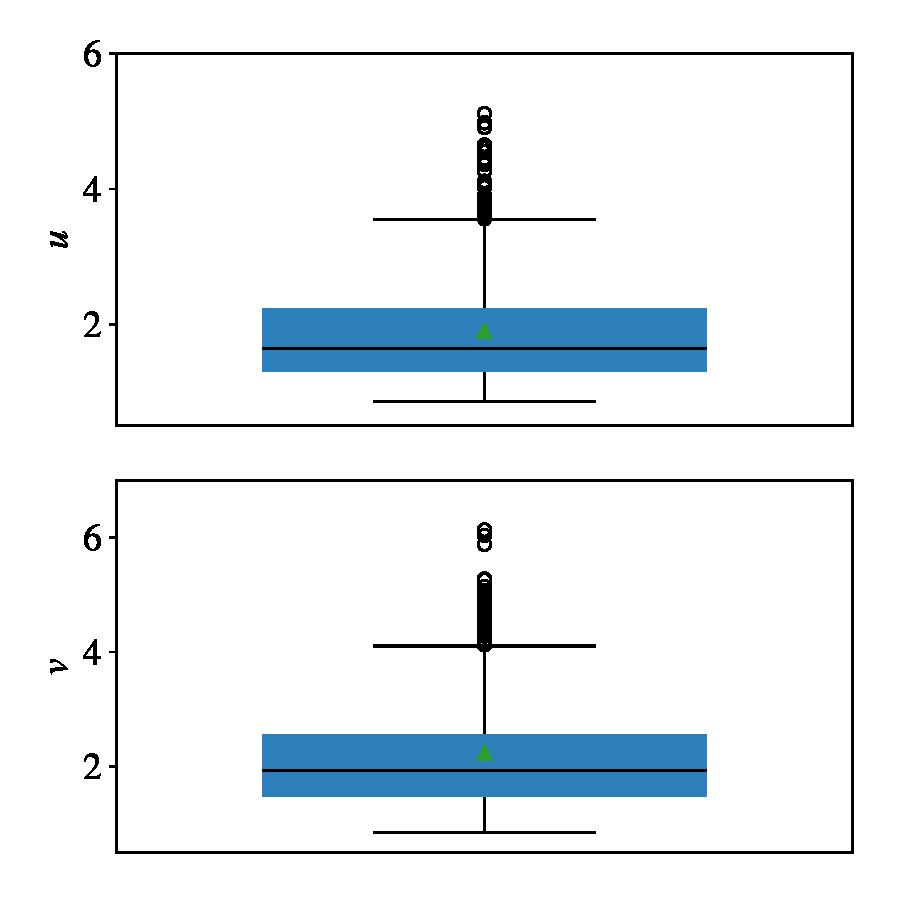
\includegraphics[width = 0.3\linewidth]{fig/eva_graphs/boxplot_tbased_uv_err_std_fr1_room.pdf}} \\
\subcaptionbox{fr1 360}{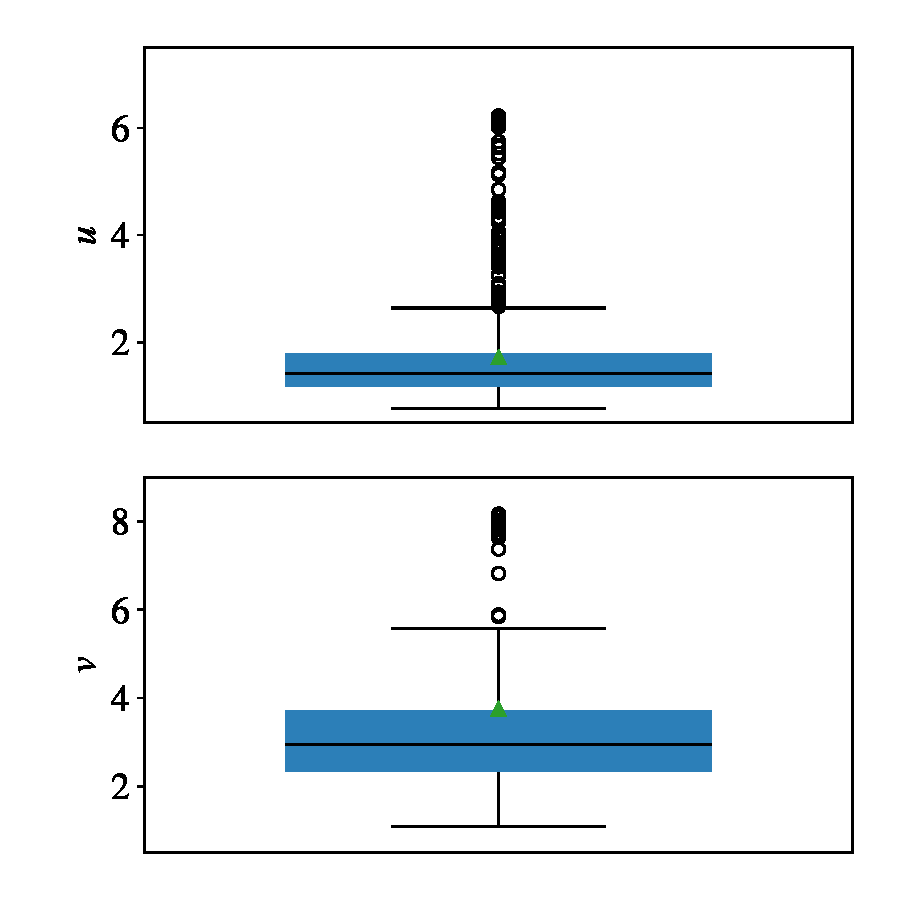
\includegraphics[width = 0.3\linewidth]{fig/eva_graphs/boxplot_tbased_uv_err_std_fr1_360.pdf}} &
\subcaptionbox{fr1 desk}{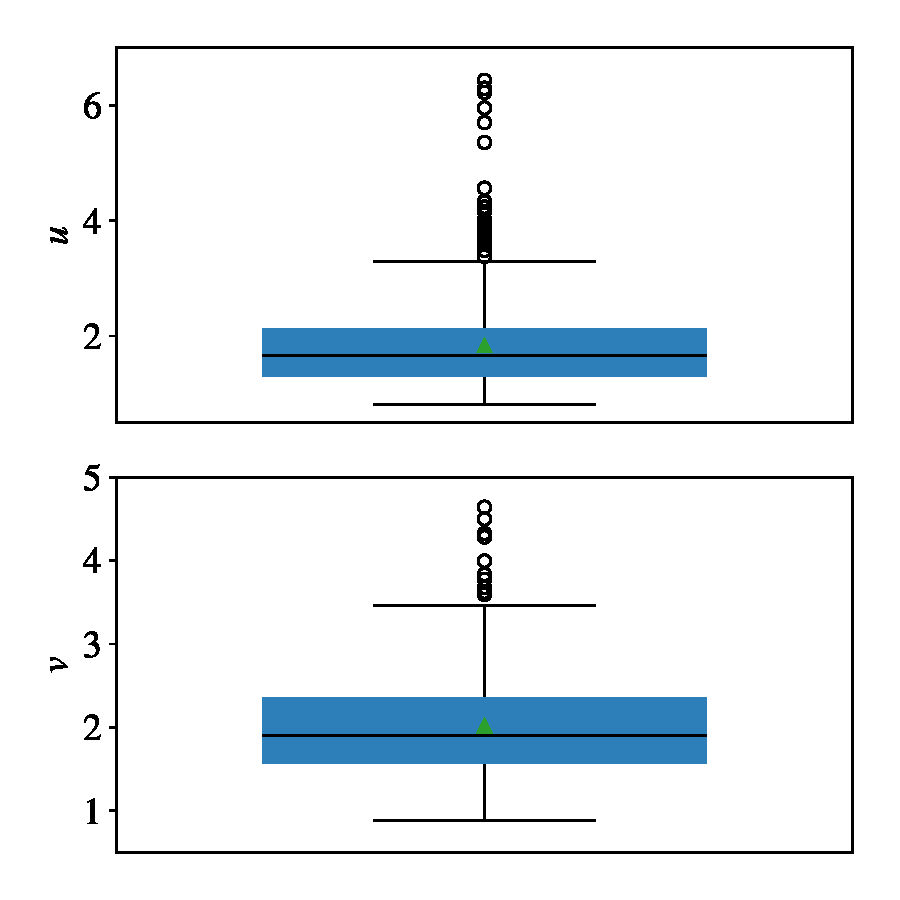
\includegraphics[width = 0.3\linewidth]{fig/eva_graphs/boxplot_tbased_uv_err_std_fr1_desk.pdf}} &
\subcaptionbox{fr1 desk2}{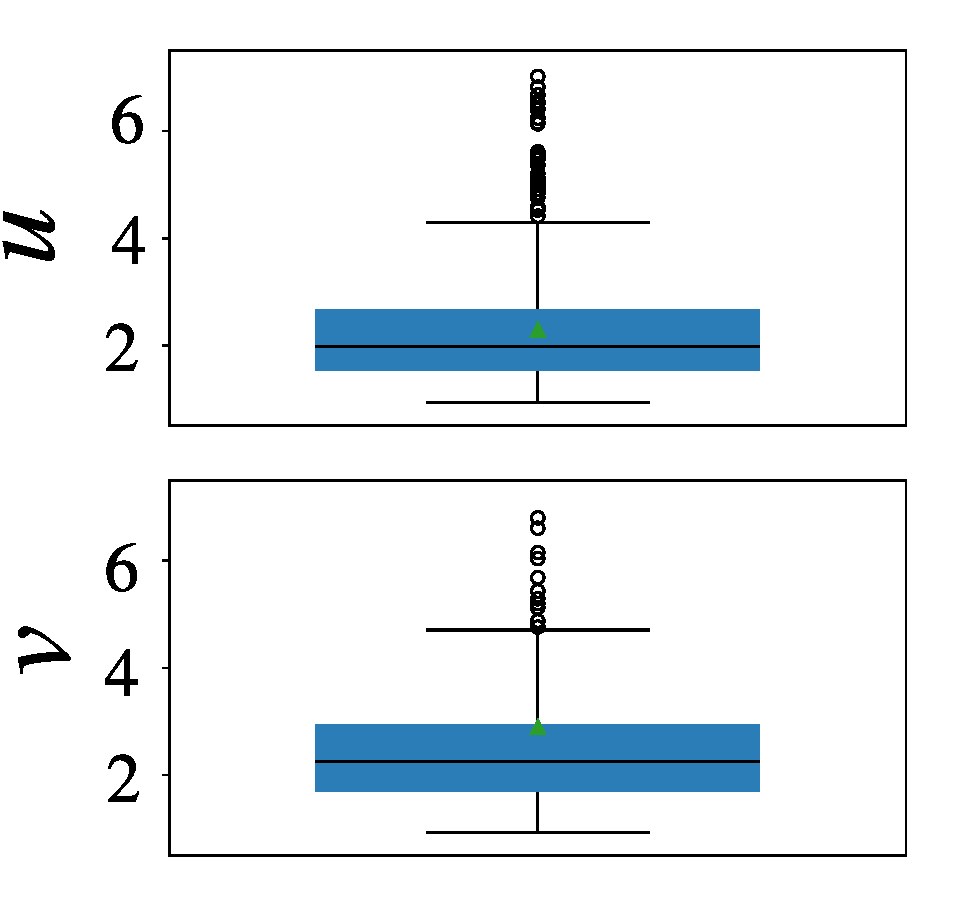
\includegraphics[width = 0.3\linewidth]{fig/eva_graphs/boxplot_tbased_uv_err_std_fr1_desk2.pdf}}
\end{tabular}
\caption[Boxplots of The Standard Deviations of Pixel Errors]
{Boxplots of The Standard Deviations of Pixel Errors in Different Datasets}
\label{fig:boxplot_time_based_std_all_datasets}
\end{figure}

To cover the worst case scenario, we take pixel uncertainty as $\sigma_u=8$ 
and $\sigma_v=8$ from fr1 rpy and fr1 desk2 datasets since the largest error 
occurs in these two datasets.  Finally, we form a covariance matrix 
$\mathbf{Q_{uvz}}^{(k,i)}$ of a point feature based on the experimental 
analysis that we conducted in this section.

\subsection{Evaluation of Estimated Covariance}\label{sc_cov_eval}

Similar to simulation data, we calculate NEES for the covariance of the estimated 
poses after running the CoVO algorithm with 6 different datasets. 
Note that we set standard deviation of pixel uncertainty according to 
the largest value $\sigma_u=8$ and $\sigma_v=8$ which was 
determined in the previous section.
Also, we scale resulting covariance $\mathbf{Q}_{\mathbf{tq}}^{k,k+1}$
with the $\phi=4^2$ to compensate for the errors caused by the linearization 
after each optimization for consecutive frames.
Under these parameterizations, we run the algorithm and calculate 
the histogram of NEES and ANEES for the selected datasets. 
The resulting histograms are illustrated in \ref{fig:hist_nees_all_datasets} and 
their ANEES are given in Table \ref{tb:anees_all_datasets}.


% Histogram of NEES with all datasets!
\begin{figure}[H]
\begin{tabular}{ccc}
\centering
\subcaptionbox{fr1 xyz}{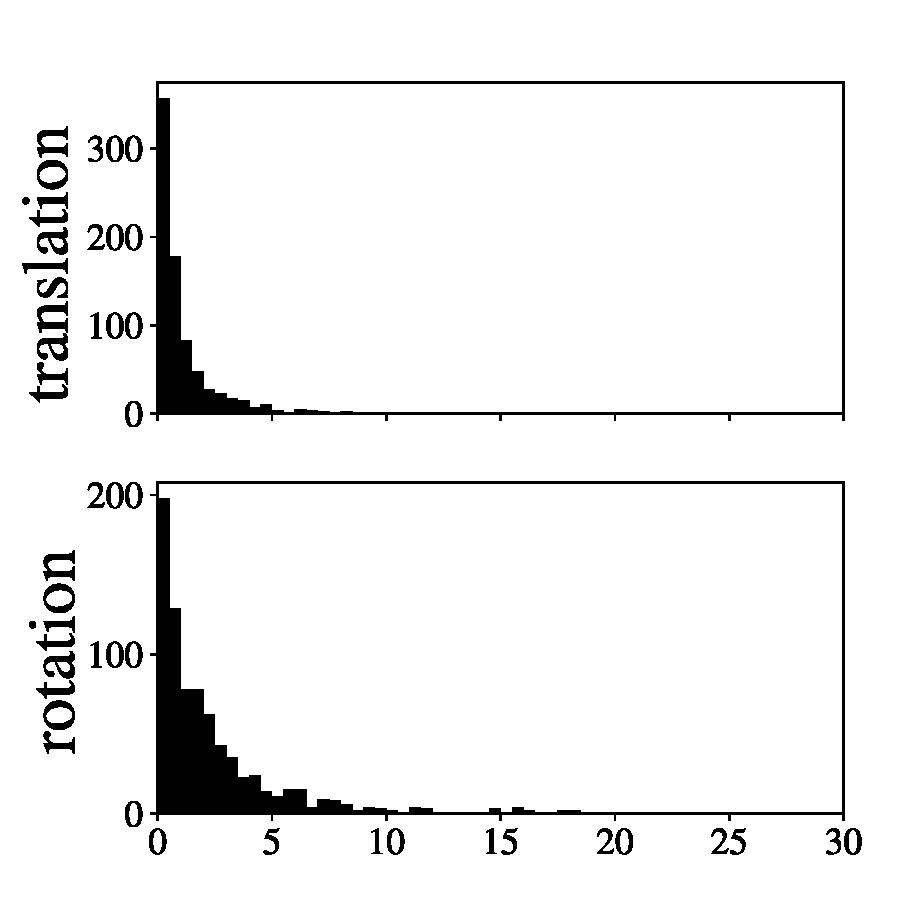
\includegraphics[width = 0.3\linewidth]{fig/eva_graphs/tum_fr1_xyz_hist_nees.pdf}} &
\subcaptionbox{fr1 rpy}{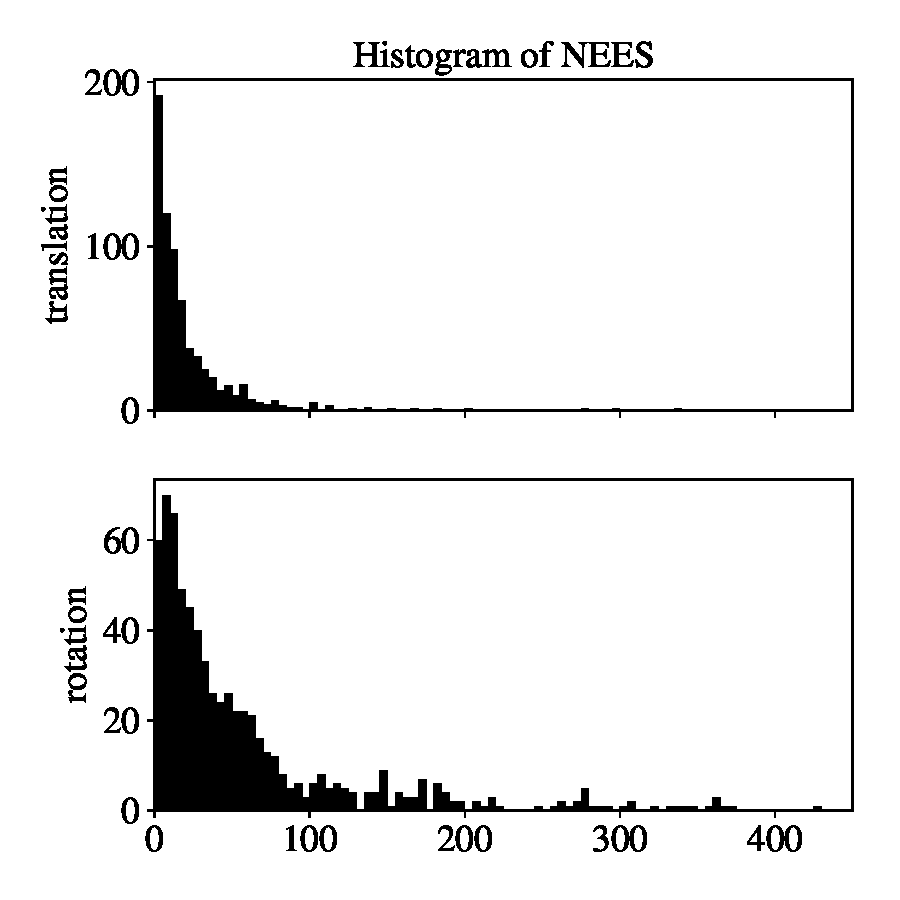
\includegraphics[width = 0.3\linewidth]{fig/eva_graphs/tum_fr1_rpy_hist_nees.pdf}} &
\subcaptionbox{fr1 room}{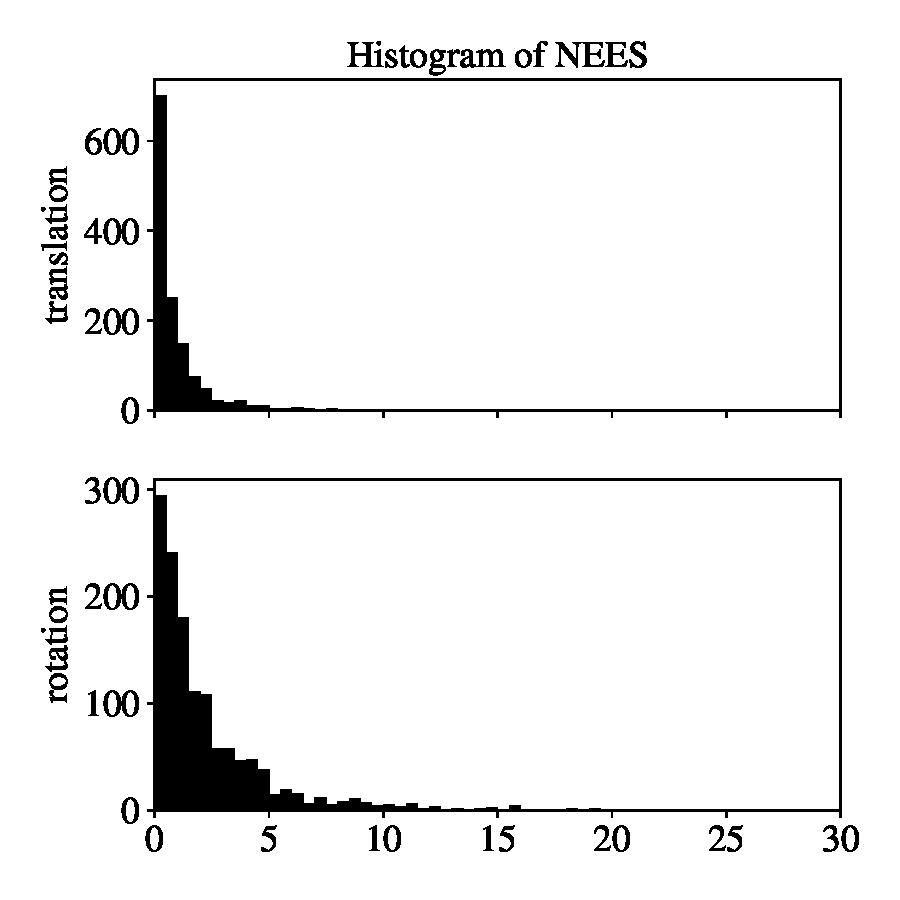
\includegraphics[width = 0.3\linewidth]{fig/eva_graphs/tum_fr1_room_hist_nees.pdf}} \\
\subcaptionbox{fr1 360}{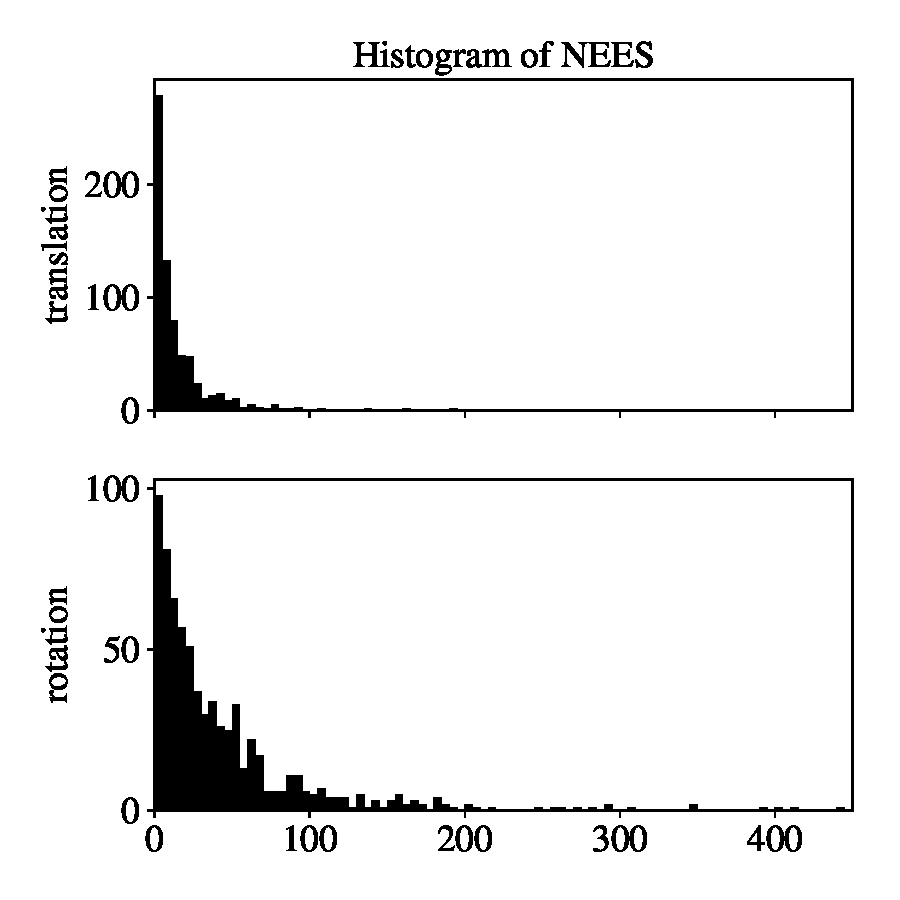
\includegraphics[width = 0.3\linewidth]{fig/eva_graphs/tum_fr1_360_hist_nees.pdf}} &
\subcaptionbox{fr1 desk}{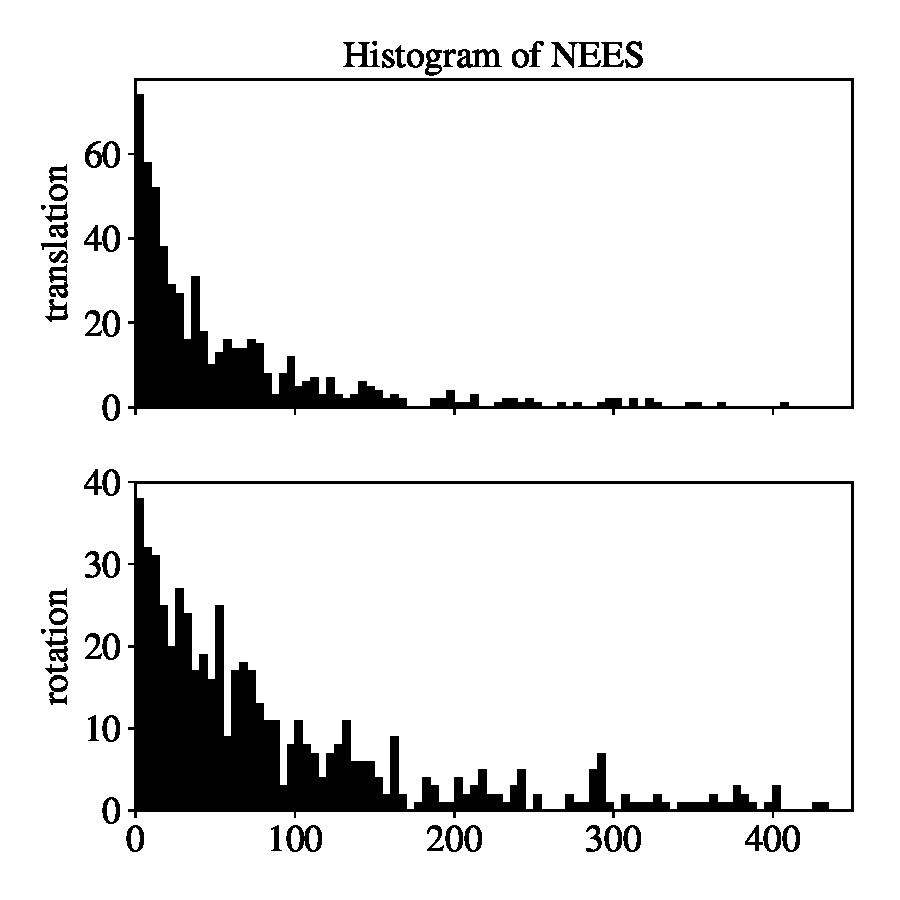
\includegraphics[width = 0.3\linewidth]{fig/eva_graphs/tum_fr1_desk_hist_nees.pdf}} &
\subcaptionbox{fr1 desk2}{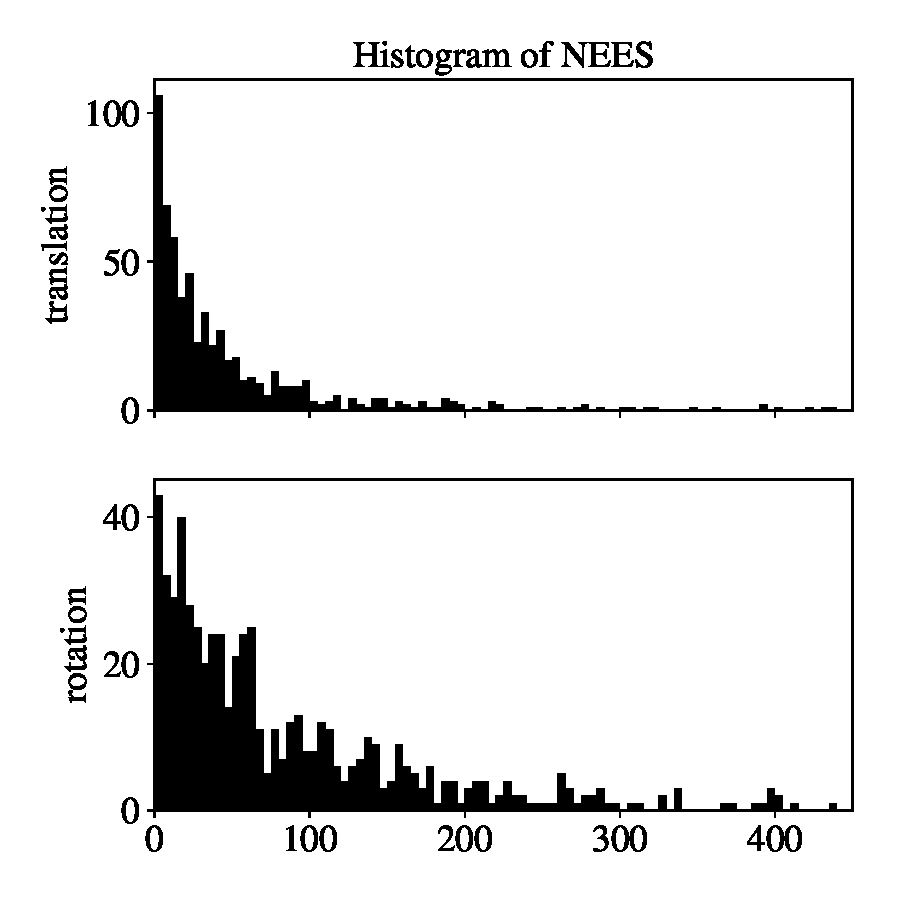
\includegraphics[width = 0.3\linewidth]{fig/eva_graphs/tum_fr1_desk2_hist_nees.pdf}}
\end{tabular}
\caption{Histogram of NEES in Different Datasets}
\label{fig:hist_nees_all_datasets}
\end{figure}

We observe that covariances of the translation estimations are conservative, 
which is acceptable in VO systems. However, covariance of the rotation estimation 
result in being overconfident for 3 datasets; i.e., 'fr1 360', 'fr1 desk' and 'fr1 room'.
Thus, we can say the estimator is \textit{inconsistent} for the rotation, 
as opposed to the translation providing \textit{consistent} covariance 
estimations.
In literature, the accuracy and consistency of the estimation in the VO 
algorithm 
are compared with the translation since it already includes the effect of 
the rotation (see notation \eqref{eq:translation_cam}). 
At the moment, the exact reason why the covariances of the rotation parts are 
estimated 
poorly is unknown to me. Therefore, the proposed CoVO algorithm needs an 
improvement for estimating the covariance of the rotational part. This could 
be a future work where I need to 
analyze the quaternion algebra and manifold operation in Ceres-Solver more 
deeply to find out why the covariances of the rotation part are estimated 
inconsistent for certain datasets.

\begin{table}
\begin{center}
  \begin{tabular}[H]{l|cc|cc}
    \hline
  & Translation ANEES & Status & Rotation ANEES & Status \\
  \hline
  fr1 xyz   & 1.55 & conservative & 2.48 & conservative \\
  \hline
  fr1 rpy   & 1.08 & conservative & 3.10 & conservative \\
  \hline
  fr1 360   & 1.21 & conservative & 3.69 & overconfident \\
  \hline
  fr1 desk  & 2.88 & conservative & 4.99 & overconfident \\
  \hline
  fr1 desk2 & 2.72 & conservative & 5.30 & overconfident \\
  \hline
  fr1 room  & 0.96 & conservative & 2.65 & conservative \\
  \hline
  \end{tabular}
  \caption{ANEES in Different Datasets}\label{tb:anees_all_datasets}
\end{center}
\end{table}

% 5
\section{Comparison to FOVIS}

%subsection{Trajectory Estimation}
As for the accuracy of the estimated poses, we compare the proposed algorithm 
with FOVIS, which is a defacto VO application since it produces very accurate 
pose estimation with fast computations.
To provide an illustration of the trajectory built from relative pose estimations, 
we draw estimations results of 'fr2 desk' which is suitable to present drift effects 
and it is given in Figure \ref{fig:comp_fr2_desk} along with the boxplot 
representation
of RPEs. 

% Traj XYZ with fr2_desk Boxplot with fr2_desk
\begin{figure}[H]
\begin{tabular}{ccc}
\centering
\subcaptionbox{The 3D Trajectories}{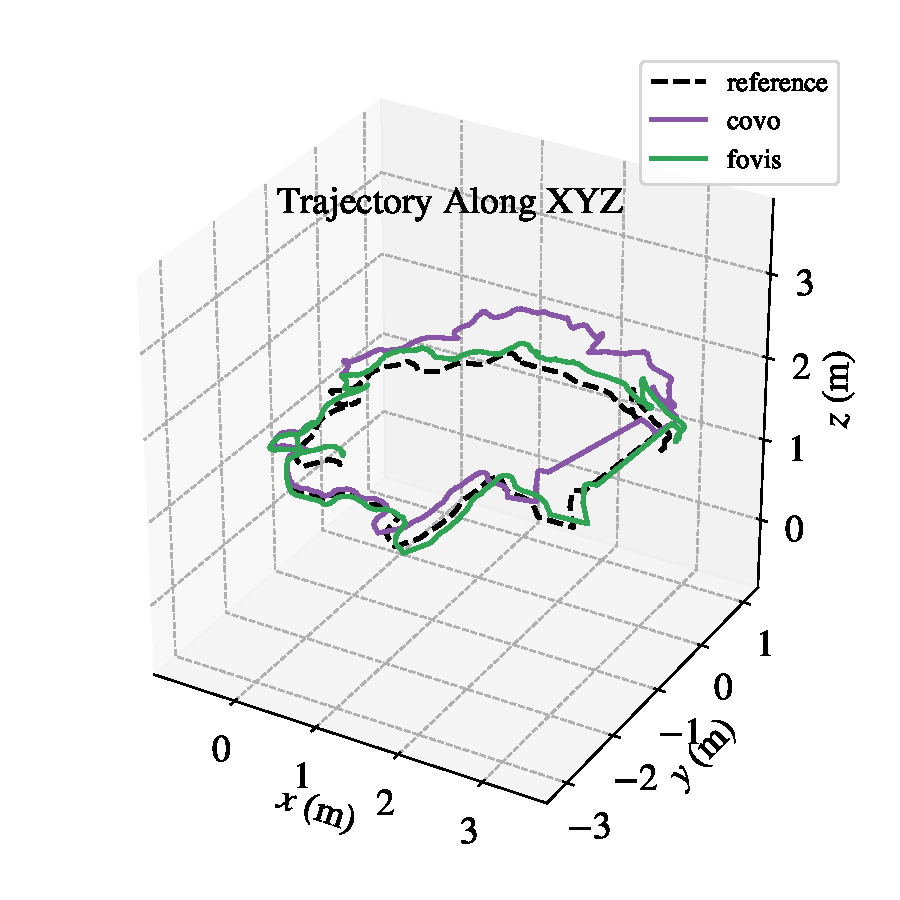
\includegraphics[width = 0.5\linewidth]{fig/eva_graphs/fovis_comp_3d_tum_fr2_desk.pdf}} &
\subcaptionbox{Boxplots of RPE}{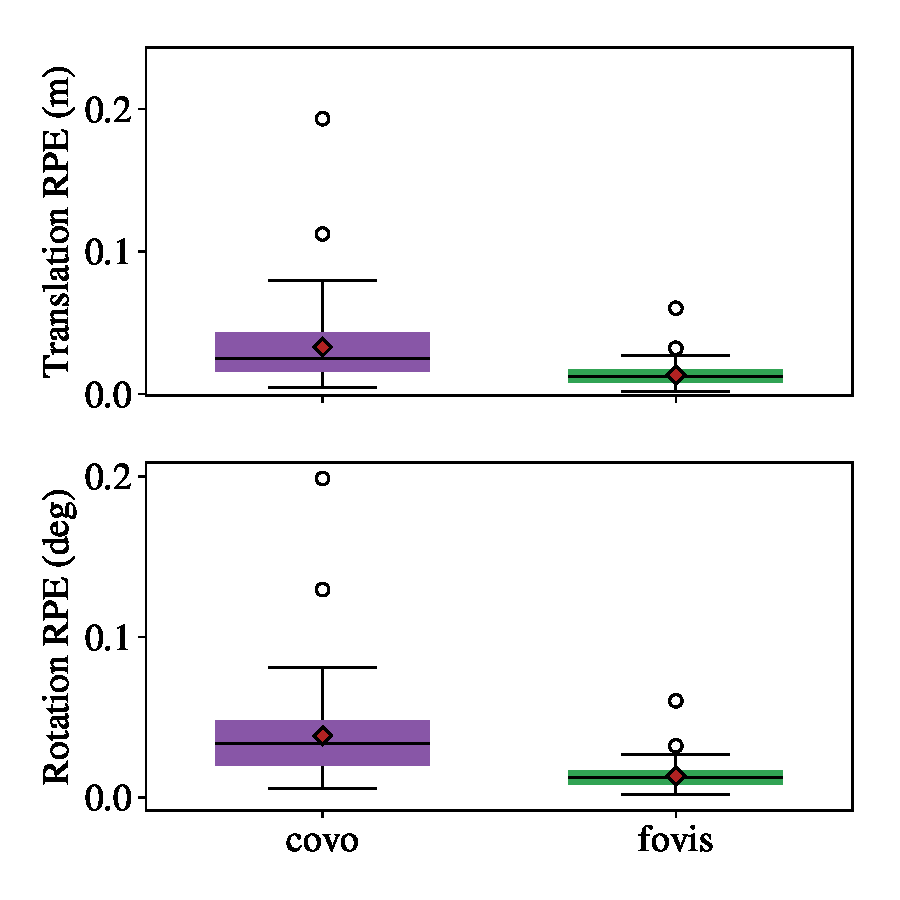
\includegraphics[width = 0.45\linewidth]{fig/eva_graphs/fovis_comp_boxplot_tum_fr2_desk.pdf}}
\end{tabular}
\caption{FOVIS versus CoVO in The TUM FR2 Desk Dataset}
\label{fig:comp_fr2_desk}
\end{figure}

We run both algorithms for the seven datasets and the resulting RMSEs of RPEs 
are given in Table \ref{tb:comp_all_dataset}. Note that we take $\Delta=30$ 
frames while calculating RPEs. Additionally, we also provide the boxplot 
representation of RPE for more explicit comparison in Figure 
\ref{fig:comp_all_dataset}.

\begin{figure}[H]
\begin{tabular}{ccc}
\centering
\subcaptionbox{fr1 xyz}{\includegraphics[width = 0.3\linewidth]{fig/eva_graphs/fovis_comp_boxplot_tum_fr1_xyz.pdf}} &
\subcaptionbox{fr1 rpy}{\includegraphics[width = 0.3\linewidth]{fig/eva_graphs/fovis_comp_boxplot_tum_fr1_rpy.pdf}} &
\subcaptionbox{fr1 room}{\includegraphics[width = 0.3\linewidth]{fig/eva_graphs/fovis_comp_boxplot_tum_fr1_room.pdf}} \\
\subcaptionbox{fr1 360}{\includegraphics[width = 0.3\linewidth]{fig/eva_graphs/fovis_comp_boxplot_tum_fr1_360.pdf}} &
\subcaptionbox{fr1 desk}{\includegraphics[width = 0.3\linewidth]{fig/eva_graphs/fovis_comp_boxplot_tum_fr1_desk.pdf}} &
\subcaptionbox{fr1 desk2}{\includegraphics[width = 0.3\linewidth]{fig/eva_graphs/fovis_comp_boxplot_tum_fr1_desk2.pdf}}
\end{tabular}
\caption{FOVIS versus CoVO With RPE Boxplots}
\label{fig:comp_all_dataset}
\end{figure}

We can say that FOVIS is more accurate than CoVO in the context of relative 
pose estimations for several reasons we can name.  FOVIS utilizes the keyframe 
scheme and different outlier rejection algorithm than RANSAC. Also, it 
provides a better initial guess to its optimizer after several refinement 
processes throughout the pipeline. Most importantly, it minimizes the 3D-to-2D 
correspondences which are less prone to settle for undesired local minimums in 
LM algorithm.

\begin{table}[H]
\caption{FOVIS versus CoVO With RMSE RPE}
\begin{center}
  \begin{tabular}{lcc}
    \hline
    & FOVIS & COVO\\
     & RMSE & RMSE\\
    \hline
    fr1 xyz   & 0.0240  & 0.0512\\ 
    \hline
    fr1 rpy   & 0.0533  & 0.0368\\
    \hline
    fr1 360   & 0.0867  & 0.1239\\ 
    \hline
    fr1 desk  & 0.0406  & 0.0665\\
    \hline
    fr1 desk2 & 0.0533  & 0.0941\\
    \hline
    fr1 room  & 0.0587  & 0.0791\\
    \hline
    fr2 desk2 & 0.0156  & 0.0428 \\
    \hline
  \end{tabular}
\label{tb:comp_all_dataset}
\end{center}
\end{table}

Lastly, this chapter has dealt with the evaluation of the proposed CoVO algorithm
regarding accuracy and consistency. Initially, we began by describing the two
main error metrics: RPE for accuracy comparisons and NEES for covariance
estimator's consistency.  Then, we provided a detailed step by step instruction
upon which the simulation environment was built. With the use of simulated
data, we identified how large noise in feature and depth measurement
contributed to covariance estimator's inconsistency. Besides this important
validation, we discovered the effect of the pseudo inliers that still exist
after an outlier rejection process. We proposed that the pixel error distance
caused by pseudo inliers can be used as the pixel uncertainty of image
features. This approach is necessary to estimate accurate metric pose covariances, which
is the primary task of this thesis.  In the final section of the chapter, we
compare the proposed CoVO algorithm with FOVIS in terms of accuracy.

\chapter{Conclusion} \label{cp_conc}

% what&how I did in 2-3 sent
This thesis was undertaken to design an error-aware RGB-D Visual Odometry
system and evaluate its credibility.  It is achieved by identifying the errors
occurring in both sensor and algorithm level and integrating them into the
optimization problem.

% outline thesis
The first step was to introduce the VO problem in the context of sensor fusion
in Chapter 1. We argued that researchers mainly targeted to improve the
accuracy of the pose estimations when developing VO systems.  On the other
hand, providing uncertainty information about their estimations is disregarded.
Knowing that the safety critical sensor applications require the covariance for
measurements, we stated the motivation; that is, we build such a VO system that
outputs a metric covariance for its pose estimation dynamically. 

After the introduction chapter, the foundational elements of a projective
camera was laid out. 
% camera model
In this respect, the geometrical models of an RGB-D camera sensor were given to
be acquainted with the working principles of such sensors.  The pinhole and
triangulation models served us as essential tools when modeling the error
characteristics of the sensors.
% typical vo pipeline
In Chapter 3, the standard pipeline of a feature based VO was studied. The
pipeline comprised of 4 fundamental processes; i.e., extracting features,
matching features, rejecting outliers and pose estimation. To model the
uncertainty of the complete system, both the systematic errors of the
sensors and the errors introduced by the image processing processes are
needed to be investigated.

% modeling uncertainties of RGB-D
In Chapter 5, two primary sources of errors are discussed such as
feature-related errors caused by outliers and depth-related errors caused by
the IR sensor.  All of these errors were combined in the conic ray model to
represent the uncertainty of 3D point features with covariances.
% optimization 
Afterward, how these uncertainties were incorporated into the optimization
process and the covariance of the estimated pose was propagated through feature
uncertainty were described in detail. With the use of the error modeling, we
provided the implementation details of the proposed algorithm which we called
CoVO.

% evaluation 
Next, Chapter 6 dealt with testing the CoVO algorithm in both the simulation
environment and real-world datasets. 
%whose purpose is to validate the correctness of the algorithm.  sim 
The experiments in simulation showed that linearization of projection function
led to inconsistency for the covariance of the estimated poses in the case of
large noise.  This issue was compensated with a heuristic method that scales
the resulting covariance accordingly.

% tum dataset
Later, TUM RGB-D datasets were used not only for testing the consistency of the
estimations with the real-world data, but also for identifying the effect of
pseudo inliers on pixel uncertainty. 
% fovis comp
At the end of the chapter, the accuracy of the proposed algorithm was compared
with FOVIS.

% limitations
Finally, several limitations to this work need to be acknowledged.  First of
all, the simulation environment was built under the assumption that the pixel
and depth uncertainties are Gaussian and there are no outliers in feature
matches. The fact that RANSAC is non-deterministic results in remaining
outliers that are greater than RANSAC's acceptance threshold. We suggested that
the remaining outliers treated as pseudo inliers.  However, once the pixel
uncertainty caused by pseudo inliers grows, it then brings out the issues with
the linearizations.  Secondly, we claimed that 
one could identify the effect of pseudo inliers by running exhaustive tests on 
many real-world datasets. 
This claim held as we observed that the pixel errors were bounded 
over seven different datasets. In the end, our solution was to take the largest
errors to cover the worst case scenario.  As a result, this design choice 
leads to us obtaining less 
adaptive covariance estimations. 

In further research, more sophisticated approaches are required, considering
heavy parameterization being done for the proposed algorithm such as the covariance
scaling factor due to linearization and the standard deviation of the
pixel errors caused by pseudo inliers. For example, a more self-tuning approach
where the parameters of the error model are also estimated based on the
resulting estimated poses could provide more dynamic uncertainty information.
Ultimately, the goal for a robust sensor fusion system is to cover
corners cases with minimum parameterization.  Thus, we need models that are
constantly predicting the probability that their predicted states are
successful.





% ***************************CP7-EVALUATION***************************
%\appendix

%\renewcommand{\thechapter}{A\arabic{chapter}}

\begin{appendices}

\chapter{Appendix} \label{cp_appendices}

\section{ORB} \label{sb_sc_orb}

One of the most strict requirements of VO is the real-time constraints since 
it is expected to work at similar to low-level inertial sensors, i.e., 
accelerometer, gyroscopes, etc.  As previously discussed, blobs detectors are 
computationally expensive. Therefore, corner-based feature detectors are more 
prevalent in VO.  \textit{ORB} \parencite{Rublee2011a} combines FAST detector 
\parencite{Rosten2006} and BRIEF descriptor \parencite{M.2010} by tuning the 
necessary 
parameters to produce robust and reproducible features.  In the end, it mostly 
performs as accurate as SIFT, plus faster. Here are steps on how to extract 
features and create descriptors with ORB: 

\begin{enumerate}
	\item \textbf{Detect corners with FAST}: FAST take each pixel on 
	the image and compare with its adjacent pixels. More specifically, 
	ORB uses FAST-9, which takes a patch of a discrete circular radius of 
	$r=9$. 
	\begin{figure}[H]
		\centering
		\includegraphics[width=0.7\linewidth,natwidth=640,natheight=640]
		{fig/ref_imgs/fast.png}
		\caption[FAST Corners]
		{Point of interest or feature points are at the intersection of edges 
			as seen for the $p,q$ and $r$ pixels and the blue lines correspond 
			to 
			the directions of the edges. For this figure, $r=4$ is taken 
			\parencite{Klette2014}.}
		\label{fig:fast_corners}
	\end{figure}
	
	The basic principle behind FAST is if the selected pixel $p$ is $\pm t$ 
	darker or brighter than adjacent pixels $r\in{1,2,\dots,n}$, we call it a 
	corner, where $t$ is our empiric threshold. Comparison pixel set $r$ is 
	chosen as a circle around in Figure \ref{fig:fast_corners}.
	
	\begin{equation}
	S_{p \rightarrow r} = 
	\begin{cases}
	S_b, & I_{p \rightarrow r} \leq I_p - t \\
	S_d, & I_p - t \leq I_{p \rightarrow r} \\
	S_s, & otherwise
	\end{cases}
	\end{equation}
	
	If a set of N contiguous pixels are either dark $S_d$ or bright $S_b$, we 
	call interest point $p$ as a corner $\mathbf{u_c} = M_c(p)$, where $M_c$ 
	is a function that returns the pixel coordinates of the corner pixel and N 
	is another empiric parameter whose purpose is to ensure a majority of the 
	comparison results either dark or bright. For more details about efficient 
	ways to 
	calculate FAST corners, I refer readers to \parencite{Rosten2006}.
	
	\item \textbf{Rank FAST corners with Harris}: After FAST detection, we 
	might get many corner candidates around the interest point. However, FAST 
	does not measure how good a corner is. Thus, we use Harris detector to 
	rank corner candidates:
	
	\begin{equation}
	\mathbf{A} = \sum_{x,y} w(x,y) 
	\begin{bmatrix}
	I_x^2 & I_xI_y \\ I_xI_y & I_y^2
	\end{bmatrix}
	\end{equation}
	
	The $\mathbf{A}$ matrix is calculated by the $I_x$ and $I_y$ partial 
	derivatives with respect to $x$ and $y$-direction on the image plane and 
	$w(x,y)$ weighting window.
	
	\begin{equation}
	R_c(\mathbf{A}) = det(\mathbf{A}) - k(trace(\mathbf{A}))^2
	\end{equation}
	
	where $det(\mathbf{A}) = \lambda_1 \lambda_2$, $trace(\mathbf{A}) = 
	\lambda_1 + \lambda_2$ and $k$ is an empiric tuning parameter. Then, we 
	use the resulting $\mathbf{A}$ to find a ranking score for each corner. 
	Now, it is possible to take top N corners from if desired.
	
	\item \textbf{Calculate orientation of corners with image moments}: ORB 
	uses BRIEF to create feature descriptors, but BRIEF fails in rotated 
	images. Therefore, ORB modifies the BRIEF by adding orientation 
	information. To get orientation, an \textit{image moment} is calculated 
	for each patch $\mathbf{S}^{(n)}$:
	
	\begin{equation}
	m_{a,b}(\mathbf{S}^{(n)}) = \sum_{x,y \in \mathbf{S}^{(n)}} x^a y^b I(x,y)
	\end{equation}
	
	where $a + b$ defines the order of the moment of $n^{th}$ patch and 
	$I(x,y)$ is the intensity of the pixel at the corner. Next, we calculate 
	the moments of order one: 
	
	\begin{equation}
	m_{1,0}(\mathbf{S}^{(n)}) = \sum_{x,y \in \mathbf{S}^{(n)}} x \cdot I(x,y) 
	\text{  ,  }
	m_{0,1}(\mathbf{S}^{(n)}) = \sum_{x,y \in \mathbf{S}^{(n)}} y \cdot I(x,y)
	\end{equation}
	
	Then, we get the orientation of the patch $\mathbf{S}^{(n)}$:
	
	\begin{equation}
	\theta(\mathbf{S}^{(n)}) = atan2(m_{0,1}, m_{1,0})
	\end{equation}
	
	\item \textbf{Form BRIEF descriptors with their corresponding 
		orientation}: Once the top N corners and their orientations are 
		detected, 
	descriptions can be formed with BRIEF. 
	
	\begin{figure}[H]
		\centering
		\includegraphics[width=0.6\linewidth,natwidth=640,natheight=640]
		{fig/ref_imgs/brief.png}
		\caption[BRIEF Descriptor]{In order to form BRIEF descriptor, one 
		needs 
			to create a group of pixel pairs from patch $\mathbf{S}^{(n)}$. 
			There are 
			two common ways to create a pair. As seen in the left figure, we 
			take the 
			feature point and pair with pixels around the circle patch. In the 
			right 
			figure, another method where we pair randomly selected pixels can 
			be 
			seen. ORB prefers the method on the right \parencite{Klette2014}.}
		\label{fig:brief}
	\end{figure}
	
	
	Then, we randomly (normal distribution) selected 256 pairs 
	$(p^{(i)}=(u^{(i)},v^{(i)},q^{(j)}=(u^{(j)},v^{(j)}))$ inside the patch 
	$\mathbf{S}^{(n)}$:
	
	\begin{equation}
	\mathbf{S}^{(n)} = 
	\begin{pmatrix}
	p^{(0)}, \dots, p^{(255)}\\
	q^{(0)}, \dots, q^{(255)}
	\end{pmatrix}
	\end{equation}
	
	Next, we rotate each $(\mathbf{p}^{(0:255)}, \mathbf{q}^{(0:255)})$ pair 
	points in $\mathbf{S}^{(n)}$ with the corresponding corner's orientation:
	
	\begin{equation}
	\mathbf{p}^{(i)}_{\theta} = \mathbf{R}_{\theta}\mathbf{p}^{(i)} \text{ and 
	} 
	\mathbf{q}^{(j)}_{\theta} = \mathbf{R}_{\theta}\mathbf{q}^{(j)}
	\end{equation}
	
	It is important to note that the authors in \parencite{Rublee2011a} 
	suggested 
	to rotate each point in increments of 2$\pi$/30. Therefore, orientation 
	$\theta$ is mapped to nearest multiple of 2$\pi$/30. To form steered (or 
	rotated) BRIEF descriptors, we compare pixel densities of pair points that 
	are selected randomly:
	
	\begin{equation*}
	\tau(\mathbf{p}^{(i)}_{\theta},\mathbf{q}^{(j)}_{\theta}) := 
	\begin{cases}
	1  & I(\mathbf{p}^{(i)}_{\theta} < I(\mathbf{q}^{(j)}_{\theta}),\\
	0  & I(\mathbf{p}^{(i)}_{\theta} \geq I(\mathbf{q}^{(j)}_{\theta})
	\end{cases}
	\end{equation*}
	
	Finally, we sum comparison results in the binary form to get the 
	descriptor  
	of the patch $\mathbf{S}^{(n)}$:
	
	\begin{equation}
	\mathbf{D}^{(n)} = f(\mathbf{S}^{(n)}) := \sum_{0\leq i,j \leq 255} 
	2^{i-1}\tau (\mathbf{p}^{(i)}_{\theta},\mathbf{q}^{(j)}_{\theta})
	\end{equation}
	
\end{enumerate}


\section{RANSAC} \label{sb_sc_ransac_app}

The model being fitted in 
RANSAC \parencite{Fischler1981b} is elements of a \textit{homography matrix}, 
which transforms a 2D 
image point to another 2D image point.  Remember that we have feature matches 
from image pairs. One of the pair is the transformed version of the other 
pair.  We can model this relationship in the following way:

\begin{equation}\label{eq:homography_full}
k
\begin{bmatrix}
\hat{u}^{(i)} \\ \hat{v}^{(i)} \\1
\end{bmatrix}
=
\mathbf{H}
\begin{bmatrix}
u^{(i)} \\ v^{(i)} \\1
\end{bmatrix}
=
\begin{bmatrix}
h_{00} & h_{01} & h_{02} \\
h_{10} & h_{11} & h_{12} \\
h_{20} & h_{21} & h_{22}
\end{bmatrix}
\begin{bmatrix}
u^{(i)} \\ v^{(i)} \\1
\end{bmatrix}
\end{equation}

The goal is to fit parameters of $\mathbf{H}$ with the selected subset of the 
matching under the condition where majority of selected point matchings are 
inliers. In this way, we can easily detect outliers by testing whether they 
fit model parameters or not. To make notation \eqref{eq:homography_full} 
more 
obvious, we form the following linear system of equations:

\begin{equation}
\underbrace{
	\begin{bmatrix}
	u^{(i)} & v^{(i)} & 1 & 0 & 0 & 0 & -\hat{u}^{(i)}u^{(i)} & 
	-\hat{u}^{(i)}v^{(i)} -\hat{u}^{(i)}\\
	0 & 0 & 0 & u^{(i)} & v^{(i)} & 1 & -\hat{v}^{(i)}u^{(i)} & 
	-\hat{v}^{(i)}v^{(i)} -\hat{v}^{(i)}
	\end{bmatrix}}_{\mathbf{A}}
\underbrace{
	\begin{bmatrix}
	h_{00} \\ h_{01} \\ h_{02} \\ h_{10} \\ h_{11} \\ h_{12} \\ h_{20} \\ 
	h_{21} \\ h_{22}
	\end{bmatrix}}_{\mathbf{h}}
= 
\begin{bmatrix}
0\\0
\end{bmatrix}
\end{equation}

The first step of RANSAC is to select a subset that contains a minimum number 
of matching points to determine the parameters of the model. In homography 
$\mathbf{H}$ case, we need at least 4 point pairs 
$(\mathbf{u}=(u^{(i)},v^{(i)}),\mathbf{\hat{u}}=(\hat{u}^{(i)},\hat{v}^{(i)}))$
to solve this linear system of equation. However, due to the noise, we 
require more than 4 point pairs, but this makes the problem over-determined. 
Therefore, we might find an approximated solution by solving the least squares 
problem. Hence, we minimize so-called \textit{algebraic distance error}:

\begin{equation}
\argmin_h || \mathbf{Ah-0}||^2.
\end{equation}

In the second step, after estimating $\mathbf{h}$ parameters, we test every 
matching that is outside the subset which randomly selected at the first 
step whether they fit to the model with the certain $\mathbf{d}$ threshold we 
define:

\begin{equation}
||\mathbf{\hat{u}} - \mathbf{H}\mathbf{u}||^2 > d
\end{equation}

In the third step, we include the points that passed our test procedure in the 
second step into our subset. In the fourth and last step, we have another test 
in 
which 
we check whether the number of matching points in our subset is large enough 
to prove that we include the majority of inliers. If not, we go back to 
the first step and repeat the whole process until we fulfill the fourth step. 
As an illustration for outlier rejection, we give a simple line fitting 
example to 
visualize the iterative nature of RANSAC in Figure \ref{fig:outlier_matches}.

\begin{figure}[H]
	\centering
	\includegraphics[width=0.8\linewidth,natwidth=640,natheight=640]
	{fig/drawings/ransac.pdf}
	\caption[Outlier Rejection with RANSAC]
	{In VO, RANSAC identifies the outliers by fitting the parameters of the 
		homography matrix iteratively.  For simplicity, this figure depicts 
		the 
		outlier 
		rejection scenario with a simple line fitting example instead of 
		homography. As seen in the figure, after the number of iteration 
		$N=14$, 
		RANSAC is able to fit line by excluding the outliers in the 
		optimization 
		process. Note that we can still have outliers within the RANSAC inlier 
		threshold which is the area shaded with light blue color.} 
	\label{fig:outlier_matches}
\end{figure}


The following listing summarizes the algorithm:

\begin{algorithm}[H]
	\caption{Rejecting outlier matches with RANSAC}
	\label{algo:ransac}
	\textbf{Input} \\
	\hspace*{\algorithmicindent}S: the smallest number of points\\
	\hspace*{\algorithmicindent}N: the number of iteration\\
	\hspace*{\algorithmicindent}d: the threshold used to identify a point 
	which fits the model\\
	\hspace*{\algorithmicindent}T: the number of nearby points to notify that 
	there is a good fit\\
	\textbf{Output} \\
	\hspace*{\algorithmicindent}C: the (consensus) set of inliers \\
	\begin{algorithmic}[1]
		
		\Procedure{RANSAC}{S,N,d,T}\\
		\While{iterations $<$ N}
		\State select random sample subset of S points
		\State estimate parameters to fit homography with S
		\ForEach {points outside S}
		\State calculate the error between estimated point and measured point
		\If {error $<$ d}
		\State add the point into S
		\EndIf
		\If {S $>$ T}
		\State return C $=$ S
		\EndIf
		\EndFor
		\EndWhile
		\EndProcedure
	\end{algorithmic}
\end{algorithm}

As it is seen in List \ref{algo:ransac}, there are four empiric parameters 
that we 
need to define; S,N,d, and T. In order to make the algorithm as efficient as 
possible, these parameters must be chosen carefully. As we discussed, S is the 
subset of matchings that we randomly select, and the initial value should be 
at 
least 4 so that we can solve the least squares problem. 

For N, it is insufficient to iterate through every matching points. Thus, we 
at least select N number of matching points with respect to the following 
condition:

\begin{equation}
\text{N} = log(1-p)/log(1-(1-\epsilon)^s)
\end{equation}

where $p=0.99$ is the probability of covering all inliers, $s$ is the minimum 
number of iteration that likelihood of choosing a subset with only outliers 
and $\epsilon$ is the probability that the match is an outlier.

For d, it is chosen empirically if the distribution of outliers is unknown. If 
it is known, i.e., Gaussian with mean $\mu$ and $\sigma$, the threshold should 
be $d=5.99\sigma^2$ so that there is a 95\% probability that the point is an 
inlier.

For T, we might have a case where we reach the expected ratio of inliers; thus 
we don't have to iterate through N number of times. That means we can 
terminate it earlier if the following condition is satisfied:

\begin{equation}
\text{T} = (1-\epsilon)n
\end{equation}

where $n$ is the total number of matching points.

\section{Rigid-Body Transformations} \label{sc_rigid_body_transformations}

\textit{Rigid-body} refers to objects made of solid materials so deformation is 
neglected. We idealize it by assuming that any given two points of 
rigid-body remains constant in time regardless of external forces 
applied to it. In $\R^3$ space, a rigid-body has 6 degrees of freedom; i.e, 
3 for the position $(x, y, z)$ and 3 for the orientation $(\alpha, \beta, \gamma)$.
The motion for a rigid-body is composed of a rotation around an axis and 
a translation along an axis. 
Let
$\mathbf{x}_0=[\mathbf{p}, \mathbf{q}]^\top=[p_x, p_y, p_z, q_x, q_y, 
q_z, q_w]^\top$
be the initial pose of the frame that is fixed to the rigid-body in $\R^3$ space, 
where $\mathbf{p}_0$ represents the position and $\mathbf{q}_0$ rotation.

\subsubsection{Translation}

One can translate the rigid-body to another position with a 
$\mathbf{t}_{0,1}$ simple vector addition operation (see Figure 
\ref{fig:app_translation}):

\begin{equation}
\begin{aligned}
  \mathbf{p}_1 &= \mathbf{p}_0 + \mathbf{t}_{0,1}\\
  \begin{bmatrix} p_x^1    \\ p_y^1 \\    p_z^1 \end{bmatrix} & = 
  \begin{bmatrix} p_x^0    \\ p_y^0 \\    p_z^0 \end{bmatrix} + 
  \begin{bmatrix} t_x^{0,1} \\ t_y^{0,1} \\ t_z^{0,1} \end{bmatrix}
\end{aligned}
\end{equation}

\begin{figure}[H]
\begin{tabular}{ccc}
\centering
\subcaptionbox{p0}{\includegraphics[width = 0.45\linewidth]{fig/eva_graphs/append_p0.pdf}} &
\subcaptionbox{p1}{\includegraphics[width = 0.45\linewidth]{fig/eva_graphs/append_p1_trans.pdf}}
\end{tabular}
\caption{Translation Example in $\R^3$}
\end{figure}\label{fig:app_translation}


\subsubsection{Rotation with Quaternions}

One can rotate the rigid-body to another orientation with the 
$\mathbf{q}_{0,1}$ quaternion product (see Figure \ref{fig:app_rotation}):

\begin{equation}
\begin{aligned}
  \mathbf{q}_1 &= \mathbf{q}_{0,1} \otimes \mathbf{q}_0\\
  \mathbf{q}_1 &= [\mathbf{q}_{0,1}]_L \mathbf{q}_0\\
  \begin{bmatrix} 
    q_w^{0,1} q_w^0 - q_x^{0,1} q_x^0 - q_y^{0,1} q_y^0 - q_z^{0,1} q_z^0  \\ 
    q_w^{0,1} q_x^0 + q_x^{0,1} q_w^0 + q_y^{0,1} q_z^0 - q_z^{0,1} q_y^0  \\ 
    q_w^{0,1} q_y^0 - q_x^{0,1} q_z^0 + q_y^{0,1} q_w^0 + q_z^{0,1} q_x^0  \\ 
    q_w^{0,1} q_z^0 + q_x^{0,1} q_y^0 - q_y^{0,1} q_x^0 + q_z^{0,1} q_w^0  
  \end{bmatrix} & = 
  \begin{bmatrix} 
    q_w^{0,1} - q_x^{0,1} - q_y^{0,1} - q_z^{0,1}  \\ 
    q_w^{0,1} + q_x^{0,1} + q_y^{0,1} - q_z^{0,1}  \\ 
    q_w^{0,1} - q_x^{0,1} + q_y^{0,1} + q_z^{0,1}  \\ 
    q_w^{0,1} + q_x^{0,1} - q_y^{0,1} + q_z^{0,1}  
  \end{bmatrix}
  \begin{bmatrix} q_w^0 \\ q_x^0 \\ q_y^0 \\ q_z^0 \end{bmatrix}
\end{aligned}
\end{equation}

where $[\mathbf{q}_{0,1}]_L$ is the left quaternion product in matrix form.

\begin{figure}[H]
\begin{tabular}{ccc}
\centering
\subcaptionbox{p0}{\includegraphics[width = 0.45\linewidth]{fig/eva_graphs/append_p0.pdf}} &
\subcaptionbox{p1}{\includegraphics[width = 0.45\linewidth]{fig/eva_graphs/append_p2_rot.pdf}}
\end{tabular}
\caption{Rotation Example in $SO(3)$}
\end{figure}\label{fig:app_rotation}


\subsubsection{Transformation}

The most useful motion is the roto-translation motion, also called 
transformation (see Figure \ref{fig:app_transformation}), 
which rotates the rigid-body and then translates it:

\begin{equation}
  \mathbf{p}_1 = \mathbf{q}_{0,1} \otimes \mathbf{p'}_0 \otimes 
  \mathbf{q}^*_{0,1} + \mathbf{t'}_{0,1}
\end{equation}

\begin{equation}
  \mathbf{q}_1 = \mathbf{q}_{0,1} \otimes \mathbf{q}_0\\
\end{equation}

where $\mathbf{p'}=[0, t_x, t_y, t_z]^\top$ is treated as a quaternion of 
a vector $\mathbf{p}$ with zero scalar part.

\begin{figure}[H]
\begin{tabular}{ccc}
\centering
\subcaptionbox{p0}{\includegraphics[width = 0.45\linewidth]{fig/eva_graphs/append_p0.pdf}} &
\subcaptionbox{p1}{\includegraphics[width = 0.45\linewidth]{fig/eva_graphs/append_p3_trans_rot.pdf}}
\end{tabular}
\caption{Transformation Example in $SE(3)$}
\end{figure}\label{fig:app_transformation}


\section{Least Squares}\label{sc_least_squares}

Throughout this thesis, least squares method empowered many different components 
of out VO system, 
such as camera calibration, RANSAC and most importantly motion estimation, 
Therefore, we will discuss underlying principles of least squares method in this section.
However, if the reader wants to dive to the theory more about the non-linear 
squares solvers, there are plenty of resources, but 
I refer the reader to \parencite{Herzog2018} since we heavily rely on this 
material 
in this section.

Ultimately, error minimization is an 
operation which wishes to get the maximum likelihood of the function. In this 
respect, 
we search the most 
likely state configuration as close as possible to its exact state. 
In optimization problems,
the goal is to find interesting points, such as local/global
maximum or local/global minimum, on the \textit{objective}
\textit{function}. However, the exact model $F(\mathbf{x})$ of a system 
mostly unknown due to the high-degree for non-linearity or lack of knowledge.
%Additionally, one needs to model the noise characteristics of measurements 
%in real-world. This noise modeling also requires an approximation. 
Thus, one can (hopefully) find a good enough solution by iteratively searching.
One way to solve such problems effectively is to generate a quadratic model of 
the objective function around initial guess $\mathbf{x}^0$ and iterate
through the function using \textit{Newton's methods} or its variations.
For example,
an optimal solution (or an interest point)
Figure \ref{fig:lsq_multivariable_function_example} is at the local
minimum of the function that is highlighted as a red point cloud.


\begin{figure}[H]
	\centering
  \includegraphics[width=0.7\linewidth,natwidth=640,natheight=640]
	{fig/lsq_multivariable_function_example.jpg}
	\caption{Local Minimum at a Convex Quadratic Function}
	\label{fig:lsq_multivariable_function_example}
\end{figure}

To elaborate the problem, we provide a regression example 
which can be in fact solved with linear least squares techniques but 
it can serve us 
as a toy example throughout our explanations for non-linear least squares 
problems.

Suppose that we have a model function $g(\mathbf{x};a)$. However,
we don't know what the $\mathbf{x}=(x_1,x_2)$ coefficients (so-called
\textit{optimization} \textit{parameters}) are and we can only
plug $a$, which is the \textit{independent} variable, into the
\textit{model} $S$ to see
how the output of the model changes given the independent variable. 
The measurements for this supposed model is given in Figure 
\ref{fig:lsq_curve_fit}(a).


\begin{figure}[H]
\begin{tabular}{cc}
\centering
\subcaptionbox{Measurements}{\includegraphics[width = 0.5\linewidth]{fig/lsq_curve_fit_measurements_v2.jpg}} &
\subcaptionbox{A Fitted Line}{\includegraphics[width = 0.5\linewidth]{fig/lsq_curve_fit_operation_v2.jpg}}
\end{tabular}
\caption
{Simple Curve Fitting Example}
\label{fig:lsq_curve_fit}
\end{figure}

Our goal is now to find a function, which will fit these measurements. 
This is a typical least squares curve fitting problem.
In this problem, we initially construct a \textit{residuals function} $r_i(\mathbf{x})$ by providing
error values between model estimation $g(x;a_i)$ and dependent
variable $S_i$. In this way, the dependent variable 
represents the real world
measurements and the residuals function represents the error between the estimated value and measurement value. 

\begin{equation}
  r_i(\mathbf{x}) := g(\mathbf{x};a_i) - S_i \qquad \text{ for }  i = 1,\dots,m.
\label{eq:}
\end{equation}

The residuals function is usually squared to magnify larger error effect:

\begin{equation}
\begin{aligned}
  F(\mathbf{x}) & = \sum_{i=1}^{m} \vert r_i(\mathbf{x}) \vert^2 = 
  \sum_{i=1}^{m} \vert g(\mathbf{x};a_i) - S_i \vert^2 =
  \sum_{i=1}^{m} (g(\mathbf{x};a_i) - S_i)^2 \\
& = \begin{Vmatrix}
  \begin{pmatrix} g(\mathbf{x};a_1) - S_1 \\ \vdots \\ g(\mathbf{x};a_m) - S_m \end{pmatrix} 
\end{Vmatrix}_2^2
\label{eq}
\end{aligned}
\end{equation}

Now, one can use the \textit{sum of squared error} function to find the most likely
configuration that can minimize the errors. 

\begin{equation}
  \mathbf{x}^* = \argmin_{\mathbf{x}} F(\mathbf{x}) = 
  \sum_{i=1}^{m} (g(\mathbf{x};a_i) - S_i)^2, 
  \quad \mathbf{x} \in \R^2
\label{eq}
\end{equation}

At this point, the objective function is ready to be handed over to 
to any \textit{gradient-descent} or 
\textit{Newton's} method solvers.
These solvers will try to find the
\textit{optimal} solution $\mathbf{x}^*$ by minimizing the objective function.

\begin{equation}
  \text{Minimize} \quad \sum_{i=1}^{m} (g(\mathbf{x};a_i) - S_i)^2, 
\quad \mathbf{x} \in \R^2
\label{eq}
\end{equation}

Essentially, what the least squares solvers, which is a special type of 
non-linear optimization problem, 
do is to travel from the initial guess point to the nearest local minimum 
on the objective function. 
For instance, we set  
the initial guess of our curve fitting problem 
as optimization parameters $\mathbf{x}=(4,4)$. 
Then, the solver will 
manage to descent a local minimum point 
$\mathbf{\mathbf{x^*}}=(1.9,2.1)$. 
At the end, if we place the solution into our model function, we
get the $g(\mathbf{x};a)=1.9+2.1a$. With this line equation, we can draw the resulting fitted line 
as shown in Figure \ref{fig:lsq_curve_fit}(b).
In this thesis, the non-linear least squares solver that we used to find the 
optimization 
parameters is the \textit{Levenberg-Marquardt} method and we will explain 
the algorithm in more details.

\subsection{Levenberg-Marquardt}
Levenberg-Marquardt (LM) is one of most well-known algorithm 
to solve least squares problem. It is the modified version of the \textit{Netwon's method}. 
In this section, we describe the idea behind 
LM algorithm. Assume that we have a $\mathbf{r}(\mathbf{x}^n)$ residuals 
function which we 
wish to model:

\begin{equation}
  \mathbf{r}(\mathbf{x}^n) = \begin{pmatrix} r_1(\mathbf{x}^n) \\ \vdots \\ r_m(\mathbf{x}^n) \end{pmatrix} \in \R^m
\end{equation}

To find a local maximum/minimum of the residuals function, we need to 
determine the first derivative that 
appears in Jacobian matrix form:

\begin{equation}
  \mathbf{J} = \frac{\partial \mathbf{r}(\mathbf{x}^n)}{\partial \mathbf{x}^n } \bigg|_{\mathbf{x}^n}
  = 
  \begin{bmatrix} 
    \vertbar & & \vertbar \\
    \frac{\partial}{\partial x_1}\mathbf{r}(\mathbf{x}^n) & \dots & \frac{\partial}{\partial x_n}\mathbf{r}(\mathbf{x}^n) \\
    \vertbar & & \vertbar
  \end{bmatrix}
  = 
  \begin{bmatrix}
    \horzbar & \nabla r_1(\mathbf{x}^n)^\top & \horzbar \\
     & \vdots & \\
     \horzbar & \nabla r_m(\mathbf{x}^n)^\top & \horzbar 
  \end{bmatrix}
  \in \R^{mxn}
\end{equation}

The least squares problem has special forms which can be exploited 
algebraically.
Here, the residuals function and its derivatives are given:

\begin{equation}
  F(\mathbf{x}) = \frac{1}{2} ||\mathbf{r}(\mathbf{x}^n)||^2 = \frac{1}{2} 
  \mathbf{r}(\mathbf{x}^n)^\top \mathbf{r}(\mathbf{x}^n) \text{  
  (Objective 
  function)}
\end{equation}\label{eq:residuals_objective}
\begin{equation}
\nabla F(\mathbf{x}^n) = \mathbf{J}(\mathbf{x}^n)^\top 
\mathbf{r}(\mathbf{x}^n) = 
\sum_{i=1}^{m} r_i(\mathbf{x}^n) \nabla r_i(\mathbf{x}^n) \text{  (First-order 
derivative)}
\end{equation}\label{eq:residuals_objective_first_der}
\begin{equation}
  \nabla^2 F(\mathbf{x}^n) = 
  \mathbf{J}(\mathbf{x}^n)^\top\mathbf{J}(\mathbf{x}^n) + \sum_{i=1}^m 
  r_i(\mathbf{x}^n) \nabla^2 r_i(\mathbf{x}^n) \text{ (Second-order 
  derivative)}
\end{equation}\label{eq:residuals_objective_second_der}


The fundamental idea behind Newton's method is to form quadratic functions 
$q(\mathbf{x})$ 
around the initial guess point $\mathbf{x}^0$ and search intelligently an optimal point at which 
the quadratic function hugs (or fits) the objective function $F(\mathbf{x})$. 
The quadratic function $q(\mathbf{x})$ is formed by approximating the objective function $F(\mathbf{x})$ 
with the second-order Taylor expansion at the given point $\mathbf{x}$.
Given 
\eqref{eq:residuals_objective}, 
\eqref{eq:residuals_objective_first_der} and 
\eqref{eq:residuals_objective_second_der}, 
we can form the quadratic model as follows:

\begin{equation}
  F(\mathbf{x}^n + \Delta \mathbf{x}) \approx
  q^n(\Delta \mathbf{x}) = 
  F(\mathbf{x}^n) + 
  \nabla F(\mathbf{x}^n) \Delta \mathbf{x} + 
  \frac{1}{2}\Delta \mathbf{x}^\top \nabla^2 F(\mathbf{x}^n) \Delta 
  \mathbf{x}
\end{equation}


As said earlier, LM is the modified version of the Netwon's method. 
The biggest difference lies on the utilization of second-order derivatives 
in the algorithm. 
The LM does not use the exact 
second-order derivative $\nabla^2F(\mathbf{x}^n)$, that appears in the special form called \textit{Hessian}, 
in its quadratic model. 
This is because it is computationally expensive to calculate Hessians. 
Instead, it uses an approximated 
Hessian model by removing $\sum_{i=1}^mr_i(\mathbf{x})\nabla^2r_i(\mathbf{x})$ 
and replacing with 
term $\lambda^n \mathbf{I}$. In this case, the approximated quadratic function will be:

\begin{equation}
  q_{LM}^n(\Delta \mathbf{x}) = 
  \frac{1}{2}\mathbf{r}(\mathbf{x}^n)^\top\mathbf{r}(\mathbf{x}^n) + 
  \mathbf{r}(\mathbf{x}^n)^\top J(\mathbf{x}^n)\Delta \mathbf{x} + 
  \frac{1}{2}\Delta \mathbf{x}^\top\mathbf{B_{LM}}^n\Delta \mathbf{x}
\end{equation}

where 
$
\mathbf{B_{LM}}^n = \mathbf{J}(\mathbf{x}^n)^\top 
\mathbf{J}(\mathbf{x}^n) + 
\lambda^n \mathbf{I}
$ 
is the approximated Hessian. Also, 
$\lambda^n>0$ is a positive number and $\mathbf{I}\in \R^{kxk}$ is the identity matrix.
After forming an approximated function at the initial guess, LM 
will search for the next point where the quadratic function converges to an  
optimal solution which is a local minimum point. An intelligent direction  
to search for a minimum point would be the direction along  
the negative gradient of the quadratic function. 
Thus, one calculates the first-order derivative as follows:

\begin{equation}\label{eq:lm_descent_direction}
  0 = 
  \nabla q^{n}(\Delta \mathbf{x}^n) = 
  \mathbf{r}(\mathbf{x}^n)^\top J(\mathbf{x}^n) + 
  \mathbf{B_{LM}}^n\Delta \mathbf{x}^n
\end{equation}


If we elaborate the above equation using the content of the Hessian model, 
we will get the following equation: 

\begin{equation}
  [\mathbf{J}(\mathbf{x}^n)^\top\mathbf{J}(\mathbf{x}^n) + 
  \lambda^n\mathbf{I}]\Delta \mathbf{x}^n = 
  -\mathbf{J}(\mathbf{x}^n)^\top\mathbf{r}(\mathbf{x}^n)
\end{equation}\label{eq:damping_full}

At this point, one solves above linear system of equations to find the traveling direction 
$\Delta \mathbf{x}^n$. Another important point is to determine the traveling 
distance on the objective function when choosing for the next point. This 
is known as \textit{step length}. It has great importance in the 
convergence time. 
In LM, the step length is determined by tuning $\lambda$ parameter, also 
known as the 
\textit{damping parameter}. However, one may ask 
how to tune the parameter 
so that it will allow the algorithm to converge to a local minimum efficiently 
and accurately. This is done by performing the \textit{progress ratio} test:

\begin{equation}\label{eq:lm_progress_ratio}
  \rho^n = \frac{F(\mathbf{x}^n) - F(\mathbf{x}^n+\Delta \mathbf{x})}{q_{LM}^n(\mathbf{0})-q_{LM}^n(\Delta \mathbf{x})} =
  \frac{\text{actual decrease in objective } F(\mathbf{x})}
  {\text{predicted decrease by model } q_{LM}^n(\Delta \mathbf{\mathbf{x}})}
\end{equation}

Based on the $\rho^n$, one creates an empiric strategy:

\begin{enumerate}
  \item If $\rho^n \geq t_2$ (where $t_2$ upper boundary threshold), then it is considered as a very successful step; 
    therefore, we can even choose a smaller value for damping factor in the 
    next iteration 
    so that 
    we increase the convergence speed.
  \item If $t_1 \leq \rho^n < t_2$ (where $t_1$ lower boundary threshold), 
  then it is still a successful step but we 
    can keep the damping factor same in the next iteration so that we don't 
    miss the local minimum.
  \item If $\rho^n < t_1$, then it is a bad step; therefore, we can reject this 
    damping factor choice and choose a larger value.
\end{enumerate}

Fundamentally, this is how LM algorithm works. 
One must keep in mind that even the sophisticated LM algorithm might fail to 
converge a desired interest point on the objective function. Hence, 
there are two crucial factors on which any gradient descent based algorithm depends:
\begin{itemize}
  \item \textit{outliers} in measurement dataset,
  \item good \textit{initial guess}. 
\end{itemize}

It is important that we provide a good initial
guess and remove outliers from the dataset. 
If these two criteria do not meet, LM might converge to the
different local minimum or might not even converge to
an optimal solution. 
That being said, we can now summarize the algorithm into five steps:

\begin{enumerate}
  \item Build the quadratic model $q_{LM}^n(\Delta \mathbf{x}^n)$ of the objective function,
  \item Compute the descent direction $\Delta \mathbf{x}^n$ by solving the linear system of 
    equations in \eqref{eq:lm_descent_direction},
  \item Calculate the progress ratio $\rho^n$ in \eqref{eq:lm_progress_ratio},
  \item Choose the next damping factor $\lambda^{n+1}$ according to progress ratio test,
  \item Set the next iteration based on progress ratio test:
    $\\ \text{  if } \rho^n < t_1 \rightarrow \mathbf{x}^{n+1}:=\mathbf{x}^n +\Delta \mathbf{x}^n \text{ (step accepted) }\\ 
    \text{  if }\rho^n > t_1 \rightarrow \mathbf{x}^{n+1}:=\mathbf{x}^n \text{ (step rejected)}$.
\end{enumerate}



\section{Least Squares on a Manifold}\label{sc_lsq_manifold}

A manifold is a special topological space whose local spaces resemble a 
Euclidean.
In fact, manifolds are a vast topic in differential geometry, but
we will explain how least squares optimization on 
a manifold works practically in the context of VO. The formulations and 
derivations are mostly taken from \parencite{Sol2016}. However, 
the original work was implemented for the graph SLAM problem. Thus, 
we change the residuals function for the VO problem accordingly. 

The ultimate goal in VO is to find the relative pose of a camera from 
$k^{th}$ frame to $k+1^{th}$ frame. 
We define a relative pose as a state vector $\mathbf{x}_{k,k+1}$. 
Through LM algorithm, we hope to 
find an optimal solution $\mathbf{x^*}_{k,k+1}$ where the residuals are 
minimum.
Remember that we iteratively descent to the minimum by performing an 
addition operator $\Delta \mathbf{x}$ to each parameter in the state vector. 
However, one important point to note that our state vector is comprised of 
translation $\mathbf{t}_{k,k+1}$ and rotation $\mathbf{q}_{k,k+1}$. 

\begin{equation}
  \mathbf{x}^n_{k,k+1} = \begin{bmatrix} \mathbf{t}^n_{k,k+1} \\ \mathbf{q}^n_{k,k+1} \end{bmatrix} \in \R^7
  \text{ ,   } 
  \Delta \mathbf{x} = \begin{bmatrix} \Delta \mathbf{t} \\ \Delta \mathbf{q} \end{bmatrix} \in \R^6
\end{equation}

One can perform a regular $+$ addition operation with translation 
to travel on the objective function $F(\mathbf{x}_{k,k+1})$ since 
it is in Euclidean space $\R^3$ where one can add vectors to each other. 
Conversely, this does not apply for rotation 
since it is $SO(3)$ Lie group in which the elements $\phi \in \R^3$ of 
rotation 
are in the tangent space $\mathcal{R} \in SO(3)$.
A solution to this issue would be optimizing on a manifold.
Hence, we need to introduce \textit{box-plus} operator
$\boxplus : \mathcal{S} \times \R^n \rightarrow \mathcal{S}$ where $\mathcal{S}$ 
is an arbitrary manifold and $\R^n$ is a N-dimensional real value vector space. 
As illustrated in Figure \ref{fig:manifold}, 
the goal is to perform small changes that are mapped to a local neighborhood in 
its own state space:

\begin{equation}
  \mathbf{x}^{n+1} = \mathbf{x}^{n} \boxplus \Delta \mathbf{x}
\end{equation}

\begin{figure}[H]
	\centering
  \includegraphics[width=0.5\linewidth,natwidth=640,natheight=640]
  {fig/ref_imgs/sphere_manifold.png}
  \caption[Sphere Manifold]
  {Mapping a local neighborhood of the unit sphere $\mathcal{S}^2$ 
  onto the plane $R^2$. The image is taken from \parencite{Hertzberg2013}}
	\label{fig:manifold}
\end{figure}


For translating the camera with a small euclidean vector, 
one can perform regular addition since $\R^3 \times \R^3 \rightarrow \R^3$:

\begin{equation}
  \mathbf{t}^n \boxplus \Delta \mathbf{t} = 
  \mathbf{t}^n + \Delta \mathbf{t} =
  \begin{bmatrix} x^{n} \\ y^{n} \\ z^{n} \end{bmatrix} + 
  \begin{bmatrix} \Delta x \\ \Delta y \\ \Delta z \end{bmatrix}
\end{equation}

However, for rotating, the box-plus operation refers to 
$SO(3) \times \R^3 \rightarrow SO(3)$ and one can rotate in its local space 
with a small unit quaternion as follows:

\begin{equation}
  \mathbf{q}^n \boxplus \Delta \mathbf{q} = 
  \mathbf{q}^n \otimes \Delta \mathbf{q} = 
  \mathbf{q}^n \otimes 
  \begin{bmatrix} \sqrt{1-||\Delta \phi||^2} \\ \Delta \phi \end{bmatrix}
\end{equation}

How does our new state vector with a manifold effect LM algorithm? 
Remember that we form $q_{LM}(\Delta \mathbf{x})$ quadratic functions 
from residuals function 
$\mathbf{r_s}(\mathbf{x}_{k,k+1})=\mathbf{L}^\top\mathbf{r}(\mathbf{x}_{k,k+1})$
 
(see notation \eqref{eq:residuals_w_back_and_forward_matrix})
for each iteration around $\mathbf{x}^n_{k,k+1}$ by calculating Jacobian 
$\mathbf{J_{tqs}}(\mathbf{x}^n_{k,k+1})=\mathbf{L}^\top\mathbf{J_{tq}}(\mathbf{x}^n_{k,k+1})$
and 
approximated Hessian matrix 
$\mathbf{B_{LMs}}=\mathbf{J_{tqs}}(\mathbf{x}^n_{k,k+1})^\top\mathbf{J_{tqs}}(\mathbf{x}^n_{k,k+1})
 + \lambda \mathbf{I}$.
Since we modify our state vector representation 
and the corresponding updating operation, we need to modify the way we calculate 
derivatives as well. We will drop $k,k+1$ subscript from the state vector 
as we generalize the 
optimization for all pose estimations. 
Here is the quadratic function of the residuals function with the modified elements:

\begin{equation}
  F(\mathbf{x}^n \boxplus \Delta \mathbf{x}) \approx 
  q_{LM} (\Delta \mathbf{x}) = 
  \frac{1}{2}
\mathbf{r_s}(\mathbf{x}^n)^\top\mathbf{r_s}(\mathbf{x}^n) + 
\mathbf{r_s}(\mathbf{x}^n)^\top\mathbf{J_{tqsm}}(\mathbf{x}^n)\Delta 
\mathbf{x} + 
\frac{1}{2} \Delta \mathbf{x}^\top\mathbf{B'_{LMs}}(\mathbf{x}^n)\Delta 
\mathbf{x}
\end{equation}

One can apply chain rule to form the new Jacobian matrix for the manifold operation:

\begin{equation}
  \begin{aligned}
  \mathbf{J_{tqsm}}(\mathbf{x}^n) = 
  \mathbf{L} \frac{\partial \mathbf{r_s}(\mathbf{x}^n)}
  {\partial \Delta \mathbf{x}} \bigg|_{\mathbf{x}^n} & = 
  \mathbf{L} \frac{\partial \mathbf{r_s}(\mathbf{x}^n)}
{\partial (\mathbf{x}^n \boxplus \Delta \mathbf{x})} \bigg|_{\mathbf{x}^n}
  \frac{\partial (\mathbf{x}^n \boxplus \Delta \mathbf{x})}
  {\partial \Delta \mathbf{x}} \bigg|_{\mathbf{x}^n,\Delta \mathbf{x}=0} \\
  & = 
  \mathbf{L}\mathbf{J_{tq}}(\mathbf{x}^n) 
  \mathbf{M}(\mathbf{\mathbf{x}^n \boxplus \Delta \mathbf{x}})
  = 
  \mathbf{L}\mathbf{J_{tqm}}(\mathbf{x}^n)
  = 
  \mathbf{J_{tqsm}}(\mathbf{x}^n)
\end{aligned}
\end{equation}\label{eq:new_jacobian_chain_rule}

where $\mathbf{L}$ is the matrix from the Cholesky factorization of information matrix, 
$\mathbf{J_{tq}}(\mathbf{x}^n)$ is the older Jacobian matrix with the respect 
to 
older state vector where we assumed that all elements are in Euclidean space 
(see notation \eqref{eq:jacob_back_proj}), 
$\mathbf{M}(\mathbf{\mathbf{x}^n \boxplus \Delta \mathbf{x}})$ is the 
matrix that we form by taking partial derivative with respect to new state vector.
Let's investigate further by breaking the new Jacobian matrix into smaller matrices 
to understand better. For weighting the optimization process, 
we assign weights with the corresponding confidence ellipsoid of matched 
features 
from both consecutive frames by means of back- and forward-projection.

\begin{equation}
  \mathbf{L} 
  =
  \begin{bmatrix}
    \mathbf{L}^{(1)}_{k} \\
    \mathbf{L}^{(1)}_{k+1} \\
    \vdots \\
    \mathbf{L}^{(m)}_{k} \\
    \mathbf{L}^{(m)}_{k+1}
  \end{bmatrix}
\end{equation}

where $\mathbf{L}^{(i)}_{k} \text{, } \mathbf{L}^{(i)}_{k+1} \in \R^{3x3}$ are 
calculated from 
$\mathbf{\Omega_{xyz}}^{(i)}_{,k}  =  {\mathbf{Q_{xyz}}^{(i)}_{,k}}^{-1}$ 
by factorization $\mathbf{\Omega = LL^\top}$.
For each matched feature, 
the calculation of older Jacobian with back- and forward-projection is the following:

\begin{equation}
  \mathbf{J_{tq}}(\mathbf{x}^n) = \frac{\partial 
  \mathbf{r}(\mathbf{x}^n)}{\partial \mathbf{x}^n } \bigg|_{\mathbf{x}^n}
  = 
  \begin{bmatrix}
    \horzbar & \nabla \mathbf{r}^{(1)}(\mathbf{x}^n)^\top & \horzbar \\
     & \vdots & \\
     \horzbar & \nabla \mathbf{r}^{(m)}(\mathbf{x}^n)^\top & \horzbar 
  \end{bmatrix}
  =
  \begin{bmatrix}
    \mathbf{J_b}^{(1)}(\mathbf{x}^n) \\
    \mathbf{J_f}^{(1)}(\mathbf{x}^n) \\
    \vdots \\
    \mathbf{J_b}^{(m)}(\mathbf{x}^n) \\
    \mathbf{J_f}^{(m)}(\mathbf{x}^n)
  \end{bmatrix}^\top
\end{equation}

where $\mathbf{J_b}^{(i)}(\mathbf{x}^n) \text{, } 
\mathbf{J_f}^{(i)}(\mathbf{x}^n) \in \R^{3x7}$. Notice that in older state 
vector, we have 3 elements from translation and 4 elements from rotation of the 
quaternion. In total, it makes 7 unknown parameters for the old state vector. 
Also, here is the second partial derivative of the chain rule:

\begin{equation}
  \mathbf{M} (\mathbf{x}^n\boxplus \Delta \mathbf{x})
  =
  \begin{bmatrix}
    \mathbf{M_b}^{(1)}(\mathbf{x}^n\boxplus \Delta \mathbf{x}) \\
    \mathbf{M_f}^{(1)}(\mathbf{x}^n\boxplus \Delta \mathbf{x}) \\
    \vdots \\
    \mathbf{M_b}^{(m)}(\mathbf{x}^n\boxplus \Delta \mathbf{x}) \\
    \mathbf{M_f}^{(m)}(\mathbf{x}^n\boxplus \Delta \mathbf{x})
  \end{bmatrix}
\end{equation}

where $\mathbf{M_b}^{(i)}(\mathbf{x}^n\boxplus \Delta \mathbf{x}) \text{, } 
\mathbf{M_f}^{(i)}(\mathbf{x}^n\boxplus \Delta \mathbf{x}) \in \R^{7x6}$.
Whereas, when taking partial derivative with the respect to 
new state vector that has same 3 elements from translation and 3 elements from 
rotation as we choose the quaternion to be a unit.
In total, it makes 6 unknown parameters for the new state vector. 
This reduction in unknown parameters by constraining a parameter 
called \textit{local parameterization}. In this way, the convergence success 
and 
speed will be improved. 
Finally, to take the derivative with respect to new state vector, we need to consider 
Euclidean space for translation and tangent space for rotation. For translation part, 
we don't have any further effect on the new Jacobian since we stay in the same space 
$\R^3 \times \R^3 \rightarrow \R^3$:

\begin{equation}
  \begin{aligned}
  \mathbf{M}^{(i)}_{\mathbf{b}}(\mathbf{t}^n \boxplus \Delta \mathbf{t}) = 
    \frac{\partial (\mathbf{t}^{n} \boxplus \Delta \mathbf{t})}{\partial \Delta \mathbf{t}} 
    \bigg|_{\Delta \mathbf{t} = 0} & =
  \frac{\partial (\mathbf{t}^{n} + \Delta \mathbf{t})}{\partial \Delta \mathbf{t}}
    \bigg|_{\Delta \mathbf{t} = 0} \\
    & =
      \begin{bmatrix} 
        1 & 0 & 0 \\  
        0 & 1 & 0 \\  
        0 & 0 & 1
      \end{bmatrix} = \mathbf{I}_3
  \end{aligned}
\end{equation}

For rotation part, however; we apply chain rule one more time to take its derivative 
$SO(3) \times \R^3 \rightarrow SO(3)$:

\begin{equation}
  \begin{aligned}
  \mathbf{M}^{(i)}_{\mathbf{b}}(\mathbf{q}^n \boxplus \Delta \mathbf{q}) = 
    \frac{\partial (\mathbf{q}^{n} \boxplus \Delta \phi)}{\partial \Delta \phi} 
    \bigg|_{\Delta \phi = 0} & =
\frac{\partial (\mathbf{q}^{n} \otimes \Delta \mathbf{q})}{\partial \Delta \mathbf{q}}
    \bigg|_{\Delta \phi = 0} 
    \frac{\partial \Delta \mathbf{q}}{\partial \Delta \phi} \\
    & =
    \frac{\partial (\mathbf{Q}^{+}(\mathbf{q}^{n}) \Delta \mathbf{q})}{\partial \Delta \mathbf{q}}
    \bigg|_{\Delta \phi = 0}
    \frac{\partial \begin{bmatrix} \sqrt{1-||\Delta \phi||^2} \\ \Delta \phi \end{bmatrix}}{\partial \Delta \phi}
    \bigg|_{\Delta \phi = 0} \\
    & =
\mathbf{Q}^{+}(\mathbf{q}^{n})
      \begin{bmatrix} 
        0 & 0 & 0 \\  
        1 & 0 & 0 \\  
        0 & 1 & 0 \\  
        0 & 0 & 1
      \end{bmatrix} \\
    & =
      \begin{bmatrix} 
        q_w^{n} & -q_x^{n} & -q_y^{n} & -q_z^{n}\\  
        q_x^{n} & q_w^{n} & -q_z^{n} & q_y^{n}\\  
        q_y^{n} & q_z^{n} & q_w^{n} & -q_x^{n}\\
        q_z^{n} & -q_y^{n} & q_x^{n} & q_w^{n}
      \end{bmatrix}
      \begin{bmatrix} 
        0 & 0 & 0 \\  
        1 & 0 & 0 \\  
        0 & 1 & 0 \\  
        0 & 0 & 1
      \end{bmatrix} \\ 
      & = 
      \begin{bmatrix} 
        -q_x^{n} & -q_y^{n} & -q_z^{n}\\  
        q_w^{n} & -q_z^{n} & q_y^{n}\\  
        q_z^{n} & q_w^{n} & -q_x^{n}\\
        -q_y^{n} & q_x^{n} & q_w^{n}
      \end{bmatrix} \in \R^{4x3}
  \end{aligned}
\end{equation}

Note that while rotating $\mathbf{q}^n$ with $\Delta \mathbf{\mathbf{q}}$, 
we utilize $\mathbf{Q}^{+}$ matrix multiplication of a quaternion rather Hamilton product 
for convenience.
Now, let's combine both translation and rotation part into a single matrix:

\begin{equation}
\mathbf{M}_{\mathbf{b}}^{(i)}(\mathbf{x}^n \boxplus \Delta \mathbf{x}) = 
    \frac{\partial (\mathbf{x}^n \boxplus \Delta \mathbf{x})}
  {\partial \Delta \mathbf{x}} \bigg|_{\mathbf{x}^n,\Delta \mathbf{x}=0} = 
  \begin{bmatrix} 
  \mathbf{I}_3 & \mathbf{0}_{3x3} \\ 
  \mathbf{0}_{4x4} & \mathbf{M}_{\Delta \phi}   
  \end{bmatrix}
  \in \R^{7x6}
\end{equation}

As explained, we now have the new Jacobian matrix based on a manifold operation.
Thus, we can solve the following linear system of equation for LM 
to calculate descent direction and step length:

\begin{equation}\label{eq:delta_x_step_length_manifold}
  (\mathbf{J_{tqsm}}(\mathbf{x}^n)^\top\mathbf{J_{tqsm}}(\mathbf{x}^n) 
  + \lambda^n \mathbf{I})
  \Delta \mathbf{x} =  
  -\mathbf{J_{tqsm}}(\mathbf{x}^n)\mathbf{r_s}(\mathbf{x}^n)
\end{equation}

Then, we can add corresponding small changes to the new state vector:

\begin{equation}
  \mathbf{x}^{n+1} = \mathbf{x}^{n} \boxplus \Delta \mathbf{x}
\end{equation}

Finally, we keep updating the unknown state vector after solving 
the equation \eqref{eq:delta_x_step_length_manifold} for the current iteration 
until we converge to an optimal solution as discussed in Appendices 
\ref{sc_least_squares}.

\section{Error Propagation Law} \label{sc_error_prop_law}

In state estimation applications, sensor measurements along with their uncertainty are 
usually fused together to keep the uncertainty of the estimated state vector 
bounded 
over time. 
The uncertainty is represented with a probability distribution, 
which is desired to be distributed as Gaussian. 
Let's assume that we get the $X$ measurement and the probability distribution 
$p(X)$ representing the uncertainty of the $X$ measurement. 
There is also a $f(X)=Y$ function that takes $X$ as an input and outputs 
as a $Y$. 
To estimate the uncertainty of the output $Y$, 
we map the probability distribution function $p(X)$, 
to the probability distribution function $p(Y)$ with the $f(X)$ function 
easily.
This is called 
\textit{error propagation law}. However, if $f(X)$ is a non-linear function, 
it gets slightly complicated. This one-dimensional case with non-linearity is 
illustrated in Figure \ref{fig:error_propagation}.

\begin{figure}[H]
	\centering
	\includegraphics[width=\linewidth,natwidth=640,natheight=640]
	{fig/ref_imgs/error_propagation.jpg}
\caption[The Non-linear Error Propagation]
{The Non-linear Error Propagation. The figure is taken from 
\parencite{Arras1998b}}
  \label{fig:error_propagation}
\end{figure}

Suppose that $X\sim \mathcal{N}(\mu_x, \sigma_X)$ is distributed Gaussian 
and we want to know how $\sigma$ probability bound 
$[\mu_x-\sigma_X, \mu_x+\sigma_X]$ is propagated through $f(X)$.
An approximation of $f(X)$ at $X=\mu_x$ can be represented with 
a first-order Taylor expansion:

\begin{equation}
  Y \approx f(\mu_x) + \frac{\partial f}{\partial X}\bigg|_{X=\mu_x} (X-\mu_x) 
\end{equation}

By means of this linearization technique, we are now able to determine 
$\mathcal{N}(\mu_y, \sigma_Y)$ 
with linear mapping. Let's map the mean error:

\begin{equation}
  \mu_y = f(\mu_x)
\end{equation}

The interesting part is the standard deviation mapping since it 
is used to describe the uncertainty:

\begin{equation}
  \sigma_Y = \frac{\partial f}{\partial X}\bigg|_{X=\mu_x} \sigma_X
\end{equation}

It is critical to note that propagated $(\mu_x, \sigma_X)$ are an only 
approximation to real mapping $f(X)$ function. To eliminate errors 
caused by linearization, standard deviation $\sigma_X$ 
should be small at the known $\mu_x$ mean. 

As seen, above example considers $f(X)=Y$ with a single input and output. 
On the other hand, if $\mathbf{X}=(X_1,\dots,X_n) \in \R^n$ has multiple inputs with 
multiple $f(\mathbf{X})=\mathbf{Y}=(Y_1,\dots,Y_m) \in \R^m$ outputs,
we approximate with a first-order partial derivative, which is a Jacobian 
matrix:

\begin{equation}
  \begin{aligned}
    \mathbf{Y} & \approx f(\mu_1,\dots,\mu_n) + 
    \sum_{i=1}^{n} [\frac{\partial f}{\partial X_i}(\mu_1,\dots,\mu_n)][X_i-\mu_i] \\
    \mathbf{Y} & \approx f(\mathbf{X}_{\mu_x}) + \mathbf{J}(\mathbf{X}_{\mu_x}) (\mathbf{X} - \mathbf{X}_{\mu_x})
  \end{aligned}
\end{equation}

where $\mathbf{J}(\mathbf{X}_{\mu_x})$ is the \textit{Jacobian} matrix formed by 
the partial derivatives:

\begin{equation}
  \mathbf{J}(\mathbf{X}_{\mu_x}) = \begin{bmatrix} \frac{\partial}{\partial x_j }f_i(\mathbf{X}_{\mu_x}) \end{bmatrix}_{ij} 
  = 
  \begin{bmatrix} 
    \frac{\partial}{\partial x_1}f_1(\mathbf{X}_{\mu_x}) & \frac{\partial}{\partial x_2}f_1(\mathbf{X}_{\mu_x}) & \dots & \frac{\partial}{\partial x_n}f_1(\mathbf{X}_{\mu_x}) \\
    \frac{\partial}{\partial x_1}f_2(\mathbf{X}_{\mu_x}) & \frac{\partial}{\partial x_2}f_2(\mathbf{X}_{\mu_x}) & \dots & \frac{\partial}{\partial x_n}f_2(\mathbf{X}_{\mu_x}) \\
\vdots & \vdots & \vdots & \vdots \\
    \frac{\partial}{\partial x_1}f_m(\mathbf{X}_{\mu_x}) & \frac{\partial}{\partial x_2}f_m(\mathbf{X}_{\mu_x}) & \dots & \frac{\partial}{\partial x_n}f_m(\mathbf{X}_{\mu_x}) \\
  \end{bmatrix}
  \in \R^{ixj}
\end{equation}

Now that we have the Jacobian matrix, we can propagate the errors for 
the multivariate case:

\begin{equation}
  \mathbf{Q}_y = \mathbf{J}(\mathbf{X}_{\mu_x})^\top \mathbf{Q}_x 
  \mathbf{J}(\mathbf{X}_{\mu_x})
\end{equation}

where $\mathbf{Q}$ is the covariance matrix that corresponds to uncertainty information.
In the VO case, we apply two error propagations. The first one is to convert 
feature covariances from the disparity space to the camera coordinate 
(see notation \eqref{eq:cov_xyz_prop}). Whereas, the second one converts 
the feature covariances to the pose covariance (see notation 
\eqref{eq:cov_tq_prop}).

\section{Calibration Parameters of TUM RGB-D}

\begin{table}[H]
	\caption{TUM RGB-D Calibration Parameters}
	\centering
  \begin{tabular}{c|c|c|c}
    Dataset & Parameter Name & Value & Explanation\\
    \hline
    \multirow{9}{*}{RGB TUM FR1} & $f_x$ & 517.3 & focal length along x 
    direction\\
    & $f_y$ & 516.5 & focal length along y direction\\
    & $c_x$ & 318.6 & principal offset point along x direction\\
    & $c_y$ & 255.3 & principal offset point along y direction\\
    & $k_1$ & 0.2624 & \multirow{5}{*}{the coefficients of distortion}\\
    & $k_2$ & -0.9531 & \\
    & $k_3$ & 1.1633 & \\
    & $p_1$ & -0.0054 & \\
    & $p_2$ & 0.0026 & \\
    \hline
    \multirow{9}{*}{RGB TUM FR2} & $f_x$ & 520.9 & focal length along x 
    direction\\
    & $f_y$ & 521.0 & focal length along y direction\\
    & $c_x$ & 325.1 & principal offset point along x direction\\
    & $c_y$ & 249.7 & principal offset point along y direction\\
    & $k_1$ & 0.2312 & \multirow{5}{*}{the coefficients of distortion}\\
    & $k_2$ & -0.7849 & \\
    & $k_3$ & 0.9172 & \\
    & $p_1$ & -0.0033 & \\
    & $p_2$ & -0.0001 & \\
\end{tabular}	
\label{tb:tum_calib_param}
\end{table}


\section{Tuning Parameters of CoVO}\label{sc_covo_tuning_param}

\begin{table}[H]
\caption{CoVO Parameters}
\centering
\begin{center}
  \begin{tabular}{c|c|c|p{4.5cm}}
    VO Pipeline & Parameter Name & Value & Explanation\\ \hline
    \multirow{7}{*}{ORB} & scale\_factor & 1.2 & Scale factor smoothing 
    images\\
    & n\_features & 1000 & Number of features \\
    & n\_levels & 8 & Number of pyramid levels\\
    & edge\_thres& 20 & FAST edge threshold (in pix)\\
    & filter\_score\_perc & 75 & Top N corners for matching (in \%)\\
    & wta\_k & 2 & Number of random points to form BRIEF\\
    & patch\_size & 31 & Number of pixels to form BRIEF\\ \hline
    \multirow{2}{*}{Depth Range} & depth\_near\_thres & 0.5 & Nearest depth 
    threshold (in m)\\
    & depth\_far\_thres & 5 & Farthest depth threshold (in m)\\ \hline
    Operability & insuff\_n\_features & 30 & Insufficient number of matched 
    features for VO\\ \hline
    \multirow{3}{*}{Uncertainty} & var\_u & $8^2$ & Pixel noise variance along 
    $u$ direction\\ 
    & var\_v & $8^2$ & Pixel noise variance along $v$ direction\\
    & var\_d & $\sigma_Z(Z,\theta)$
    & Depth noise variance model\\ \hline
    Pose Covariance & cov\_scale & $4^2$ & Scaling factor to keep pose 
    covariance conservative\\ \hline
    \multirow{2}{*}{Ceres} & lin\_solver\_type & DENSE\_SCHUR & Linear solver 
    type for 
    calculating the step size\\
    & cov\_solver\_type & SPARSE\_QR & Linear solver type for calculating the 
    covariance matrix\\
  \end{tabular}
	\label{tb:covo_param}
\end{center}
\end{table}

\end{appendices}

\printbibliography[heading=bibintoc]

\end{document}


